\chapter{Implementation}%
\label{chapter:methodology}

\begin{introduction}
This chapter presents the non-functional requirements and the use cases of the applications. 
\end{introduction} 


\section{Database} 


\begin{figure}[h]
  \caption{Database general diagram.}
  \centering
  \includegraphics[width=\textwidth]{figs/dbDiagrams/DbDiagramFull}
  \label{fig:figure2} 
\end{figure}

In this section i will describe the dabase structure i create to solve this problem.
To solve this problem i create a structure that devides in 5 sections:
- Maintenance \& Tasks
- Parts \& Inventory 
- Purchasing
- Services
- Vehicles \& Owners
- Users
 

\subsection{Users} 

The section users was provided by the ligthmobie's dabase structure and i used it to create users, create the roles of the users and create the group of users (client, rececionist, warehouse manager,...).



\subsection{Maintenance and Tasks} 


\begin{figure}[h]
  \caption{Database Maintenance and Tasks diagram.}
  \centering
  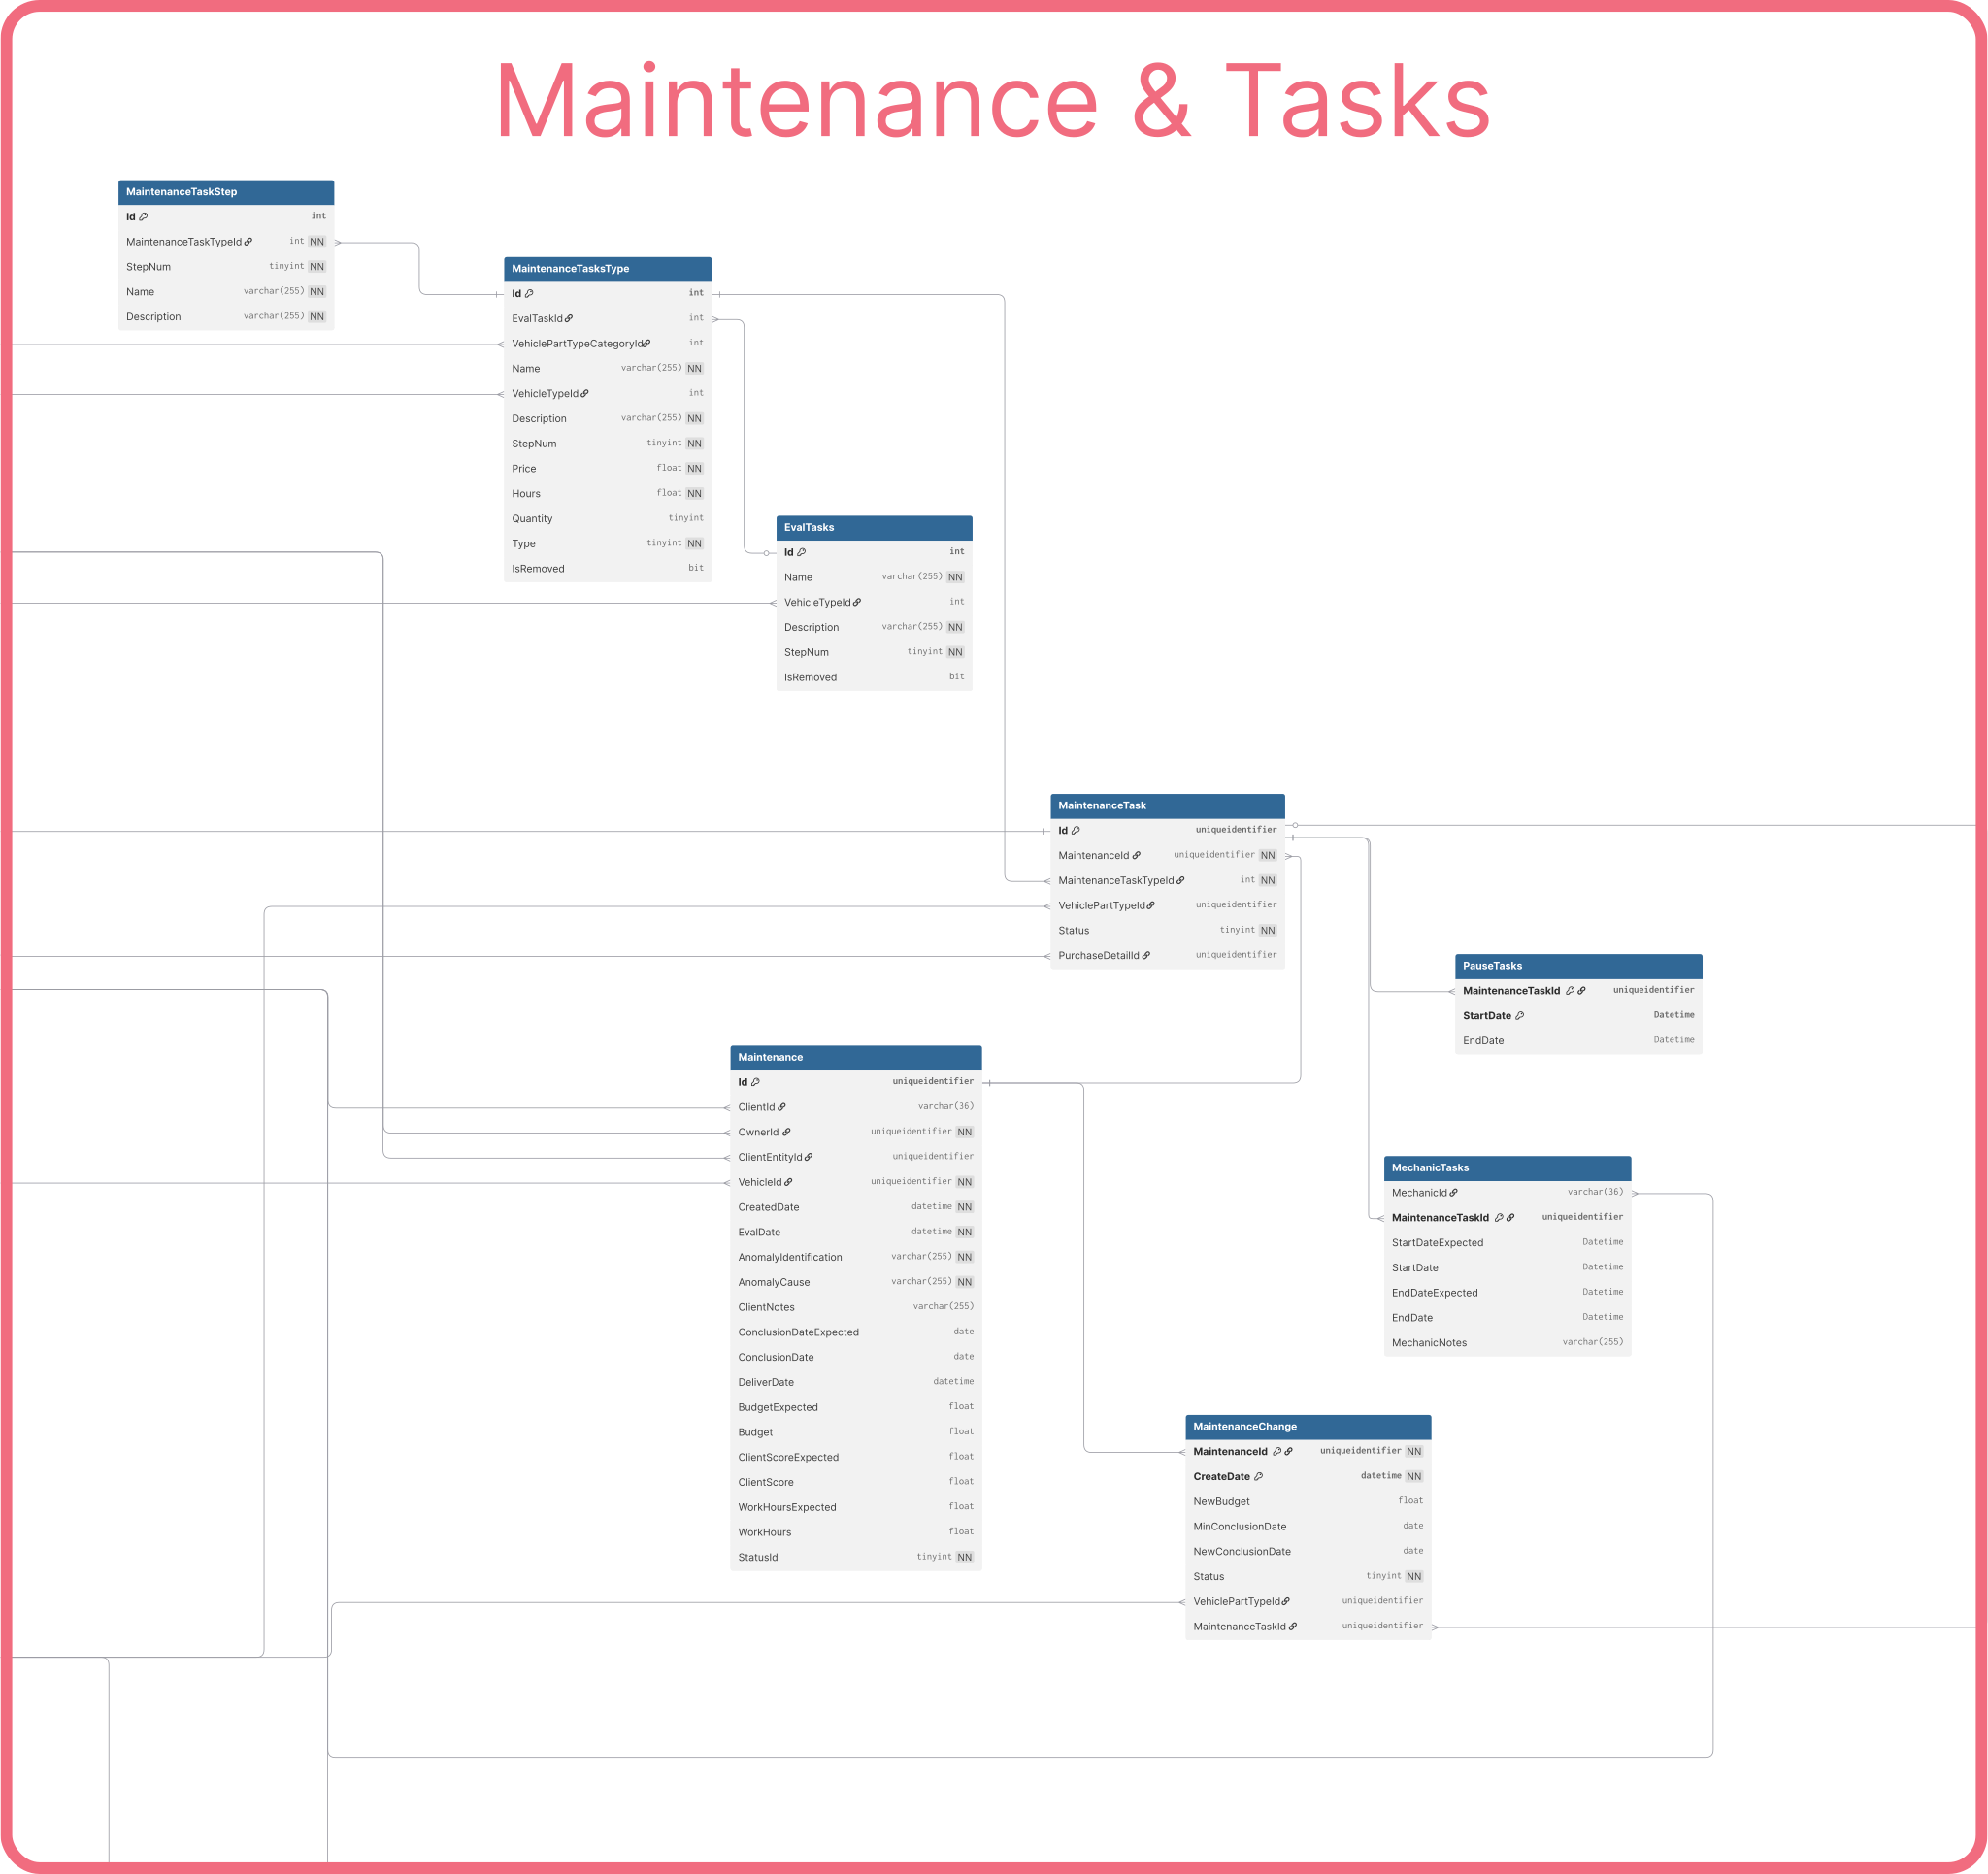
\includegraphics[width=\textwidth]{figs/dbDiagrams/Maintenance_and_Tasks}
  \label{fig:figure2}
\end{figure}

To save the information about the maintenance i created a table called the "Maintenance". This table has the following columns:
- ClientId, which is a foreign key to the AspNetUsers Table and is the table that has the information about the users of the platform.
- OwnerId, which is a foreign key to the Owners table and represents the dealership that is providing the maintenance
- VehicleId, the vehicle that is going to do the maintenance
- ClientEntityId, Optional column that connects to the Owner of a bike sharing system
- CreatedDate, that is the date of creation of the maintenance
- EvalDate, date of the evaluation date of the vehicle
- AnomalyIdentification, is a text describing the problem with the vehicle
- AnomalyCause, is a text describing the cause of the problem with the vehicle
- ClientNotes, is a text describing additional information provided by the client
- ConclusionDateExpected, is the expectedd date of the end of the maintenance agreed with the client, used to control the expectation of client for the duration of the maintenance 
- ConclusionDate, the actual date of the end of the maintenance
- DeliverDate, the date of the deliver of the vehicle to the client
- BudgetExpected, the expected budget of the maintenance agreed with the client, used to control the expectation of client for the price of the maintenance 
- Budget, the actual price of the maintenance
- ClientScoreExpected, the score of the quality of the service expected by the client
- ClientScore, the score of the quality of the service perceived by the client
- WorkHoursExpected, the number of hours expected to conclude the maintenance
- WorkHours, the number of hours to conclude the maintenance
- StatusId, the status of the maintenance. It can be WaitEvaluation, the status before the evaluation of the vehicle; waitApproval, after the evaluation of the vehicle and before the client and rececionist decide which tasks should be done, the budget of the expected budget of the maintenance and the expected conclusion date; DuringMaintenance, the status when the tasks of the maintenance are being completed; MaintenanceFinished, after all the tasks of the maintenance are completed; Delivered, when the vehicle is delivered to the client; Canceled, when the client decides to cancel the maintenance and retrieve the vehicle as it is

The maintenance is connected to the MaintenanceChange table. This table is used to save the information when a change in the maintenance occurr, like the expected conclusion date change, a task changed or the expected budget changed.
This table has the following columns:
- MaintenanceId, the identification of the maintenance which is being changed
- CreatedDate, the date of the change
- NewBudget, the new expected budget
- MinConclusionDate, the earleast date to complete the maintenance. This columns is important if, for example a part delivery is late and may only arrive on a date after the expected conclusion date.
- NewConclusionDate, the new expected conclusion date agreed with the client
- Status, the status of the maintenanceChange. It may be AskClient, when the maintenance change needs the valiation of the client; Agreed, when the client accept the changes; Refused, when the changes are refused and the maintenance keeps the same information and the previous agreement; TaskCanceled, when the client decides to cancel the task that provokes the maintenance change; MaintenanceCanceled, when the client decides to terminated the maintenance as it is.
- VehiclePartTypeId, the new part of the vehicle that from the maintenance task that is being changed
- MaintenanceTaskId, the identification of the maintenance Task that provokes the change

The maintenance is also connected with the table maintenanceTask that saves the information of the tasks from that maintenance.
This table has the following columns:
- Id, the identification of the task
- MaintenanceId, the identification of the maintenance
- MaintenanceTaskTypeId, the identification of the type of task
- VehiclePartTypeId, the identification of the type of part is used in this task
- Status, the status of the task. It may be WaitApproval, status before the approval from the client; WaitAssignment, status after the client approval but before the workshop mananger assign it to a mechanic; Invalid, status when the client rejects the task during the maintenance agreement with the rececionist; Assigned, status when the task is assigned to a mechanic; Concluded, when the task is finished; Changed, when the mechanic notes a problem with the task and suggest a change that requires the validation from the client; WaitPart, when the part needed to complete the task is not in inventory and needs to wait for it availability to be completed.
% - PurchaseDetailId, the identification of the purchase part that is requesting the part needed to complete this task. This column allows when the purchase is complete and the parts arrive the task is notified to be able to be assigned and completed.


The maintenanceTask is connected with the table pauseTasks, that keeps tracking of the pauses of the task. 
This table has a:
- MaintenanceTaskId, that identifies the task of the maintenance
- StartDate, the start date of the pause
- EndDate, the end date of the pause

It is connected to the mechanicTasks. This table has the information of the completion of the task. It has the following columns:
- MechanicId, the identification of the mechanic
- MaintenanceTaskId, the identification of the task of the maintenance
- StatDateExpected, the date the workshop manager assigned to the mechanic starts the task
- EndDateExpected, the expected date the mechanic should end the task
- StartDate, the actual date the mechanic started the task
- EndDate, the actual date the mechanic ended the task
- MechanicNote, text left from the mechanic about the task or the vehicle


The MaintenanceTask table is also connected to the MaintenanceTaskType table. This table has the information of the type of tasks exist.
It has the following columns:
- Id, identification of the task type
- EvalTaskId, the identification of the evaluation task that can generate this type of tasks. During the evaluation period of the vehicle, if the mechanic do this evaluation task, it may add this task to the maintenance
- VehiclePartTypeCategoryId, the identification of the category of parts that this task type need to be completed
- Name, the name of the task
- Description, the description of the task
- StepNum, a integer value that represents the sequence of the tasks, for example it it has the value 2, it means it is only possible to complete this task after all tasks from stepNum 0 and 1 from this maintenance are completed
- Price, the price the client must pay to complete the task
- Hours, the number of hours estimated to complete the task
- Quantity, the number of parts is needed to complete the task
- Type, the type of maintenanceTaskType this type of maintenanceTaskType is. It may be normal, a normal task or a quality task, a task to assure the quality of the vehicle before the deliver to the client
- IsRemoved, it tells if this type of task is visible or not in the platform, this virtually seems that the task is deleted on the platform, but it can be recover if needed

The maintenanceTaskType is connected to the maintenanceTaskStep, that has the information of all the steps to complete the task.
It has the following columns:
- Id, the identification of the step
- MaintenanceTaskTypeId, the identification of the task type
- StepNum, the number of the step of the task type
- name, the name of the step
- description, the description of the step and how to complete it

The maintenanceTaskType also is connected to the EvalTasks. This table has the information about the task steps used during the evaluation of the vehicle.
It has the following columns:
- Id, the identification of the evaluation task step
- Name, the name of the evaluation task step
-VehicleTypeId, the type of vehicle that this task can be applied to
- VehiclTypeId, the identification of the type of vehicle that this task step is used on
- Description, the description of the task step
- StepNum, the step number of the task step
- IsRemoved, it tells if this type of task is visible or not in the platform


\subsection{Parts and Inventory} 


\begin{figure}[h]
  \caption{Database Parts and Inventory diagram.}
  \centering
  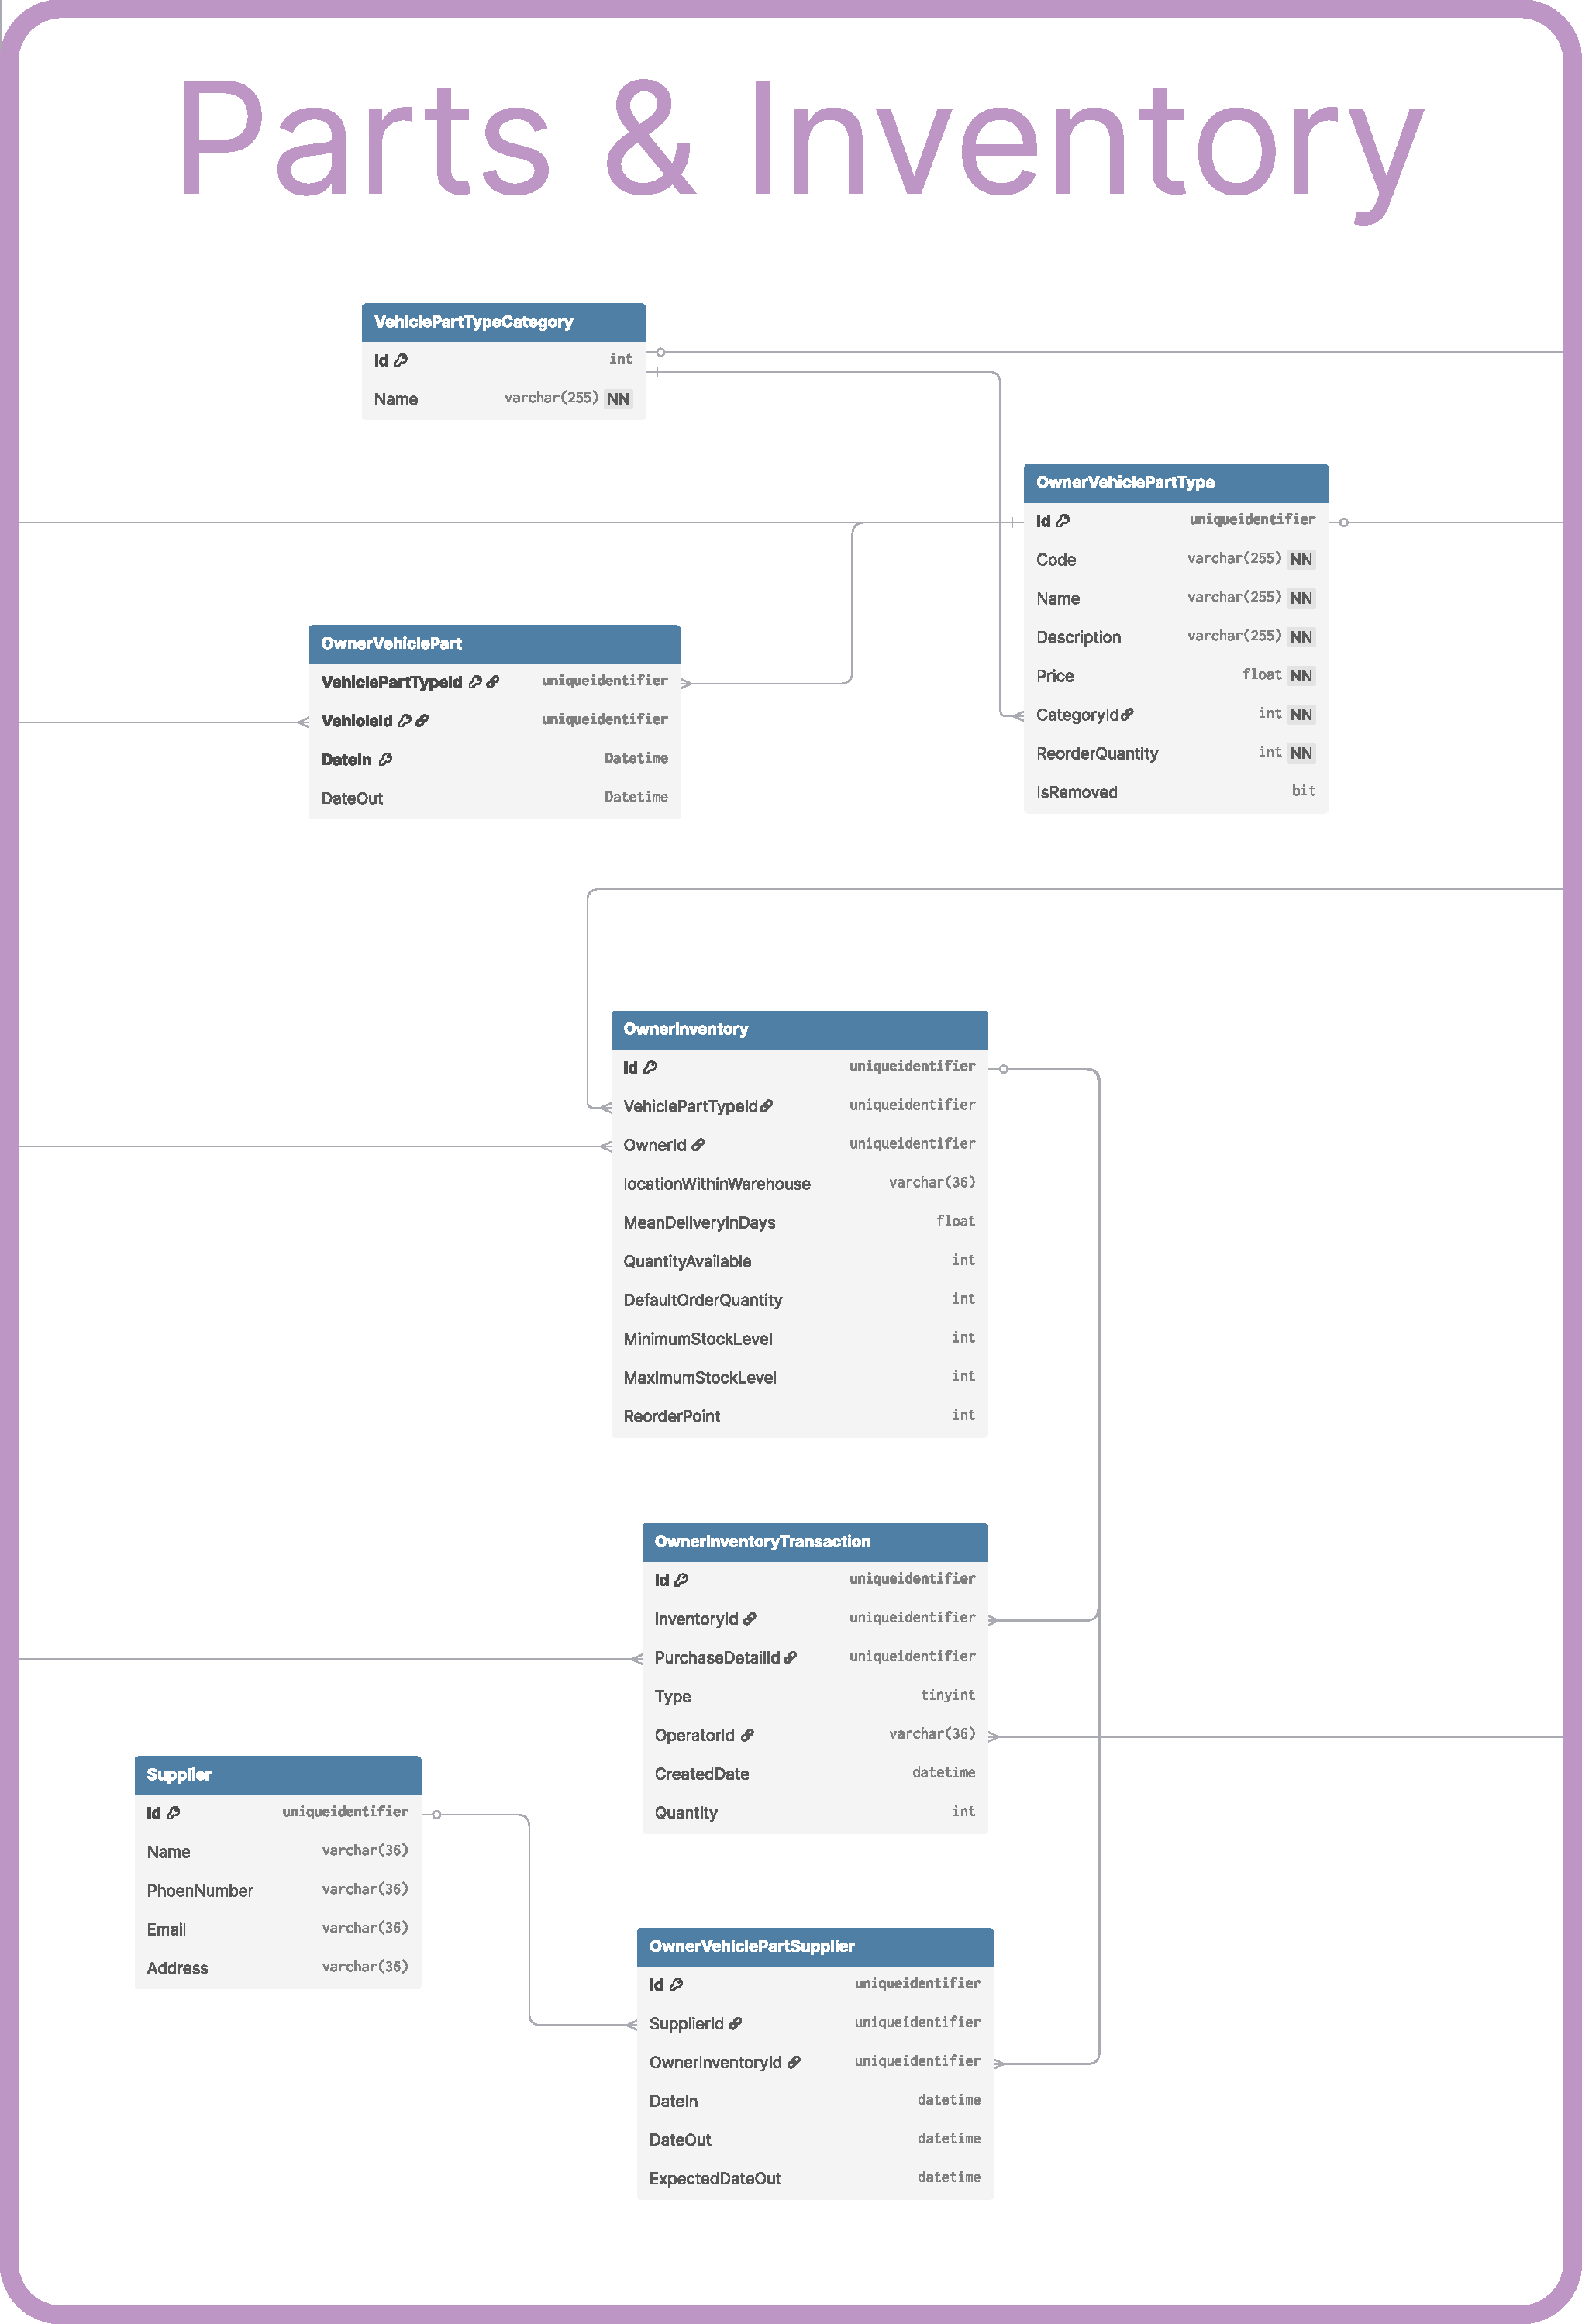
\includegraphics[width=\textwidth]{figs/dbDiagrams/Parts_and_Inventory}
  \label{fig:figure2}
\end{figure}

The inventory of the dealership is used to track the available parts on the dealership on the table OwnerInventory.
It has the following columns:
- Id, identification of the inventory
- VehiclePartTypeId, the identification of the part type of this inventory
- OwnerId, the identification of the dealership of this inventory
- LocationWithinWarehouse, is text with the code to locate the part in the warehouse of the dealership
- MeanDeliveryInDays, mean of the number of days it takes for the part to arrive at the dealership after the purchase
- QuantityAvailable, the number of parts of a specific type are available at this dealership
- DefaultOrderQuantity, the number of parts used when creating an automatic purchase for this part type when quantity on the dealership reaches a threshold
- MinimumStockLevel, the minimum number parts it the dealership should have
- MaximumStockLevel, the maximum number of parts the dealership should have
- ReorderPoint, the threshold where a purchase is created when the quantity available reaches this value

The OwnerInventory table is connected to the table OwnerInventoryTransaction, which stores the information of the sales and restock. When the quantity available changes, the action that provokes this change is saved in here.
This table has the following columns:
- Id, identification of the transaction
- InventoryId, the identification of the inventory from which occurred a sale or a restock
- PurchaseDetailId, the identification of the purchase that make the restock
- Type, if it is a restock or sale
- OperatorId, the identification of the person that provided this transaction (Warehouse Operator if it was a restock or a mechanic if it was a sale)
- CreatedDate, the date of the transaction
- Quantity, the number of parts that were added or removed from the inventory

The OwnerInventory table is also connected to the table Supplier throw the table OwnerVehiclePartSupplier.
The table supplier has the information of the suppliers of a dealership. The OwnerVehiclePartSupplier has the information of the contract between the dealership and the supplier. 
The table supplier has the following information:
- Id, the identification of the supplier
- Name, the name of the supplier
- PhoneNumber, the phonenumber of the supplier 
- Email, the email of the supplier
- Address, the address of the supplier

The OwnerVehiclePartSupplier has the following columns:
- Id, the identification of the contract
- SupplierId, the identification of the supplier
- OwnerInventoryId, the identification of the inventory of the dealership. This column identifies the dealership and the part on the contract.
- DateIn, the date that the contract starts
- DateOut, the date when the contract ended
- Quantity, the limit of parts requested in the contract
- ExpecteDateOut, the date where contract is expected to end

The OwnerInventory is also connected to the OwnerVehiclePartType that stores the type of parts exist.
This table has the following columns:
- Id, the identification of the part type
- Code, the code of the part type
- Name, the name of the part type
- Description, the description of the part type
- Price, the price of the part type
- CategoryId, the identification of category of the part type
- ReorderQuantity, the number of items per group this part must be bought with
- IsRemoved, it tells if this type of part is visible or not in the platform

This table is connected to two other tables, the VehiclePartTypeCategory and the OwnerVehiclePart.
The VehiclePartTypeCategory stores the information of the category of parts exist. 
The OwnerVehiclePart table tracks which vehicle has which parts and it already existed in the lightmobie database.
The VehiclePartTypeCategory has the following columns:
- Id, the identification of the category
- Name, the name of the category

The OwnerVehiclePart has the following columns:
- VehiclePartTypeId, the identification of the part type that the vehicle has
- VehicleId, the identification of the vehicle that has the part
- DateIn, the date when the part was inserted to the vehicle
- DateOut, the date when the part was removed from the vehicle



\subsection{Purchasing} 


\begin{figure}[h]
  \caption{Database Purchasing diagram.}
  \centering
  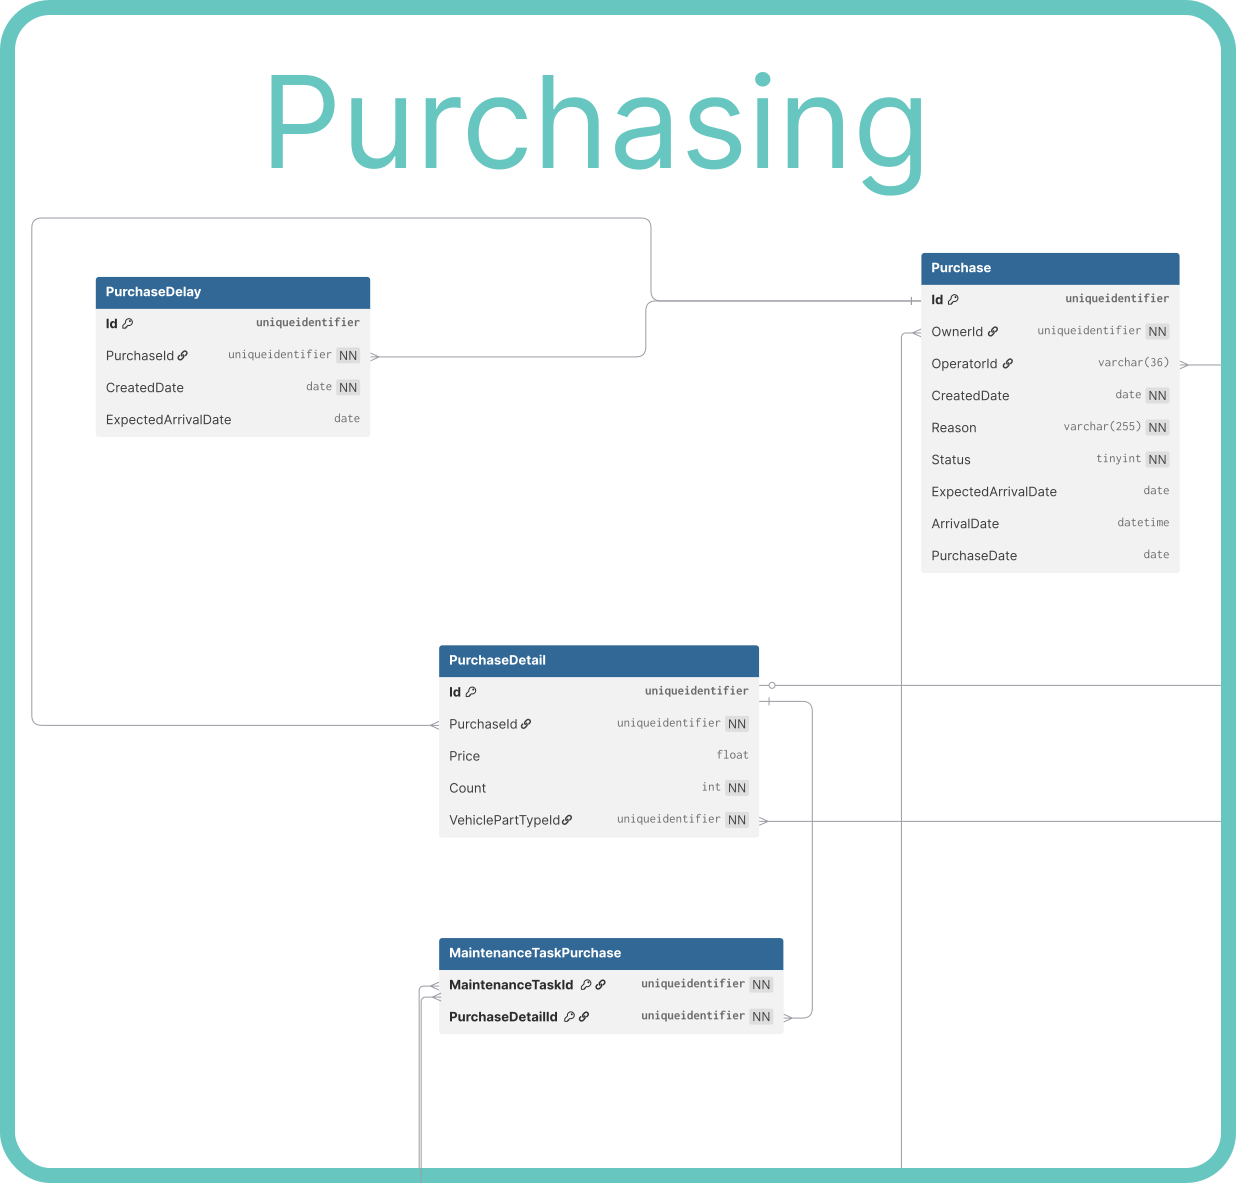
\includegraphics[width=\textwidth]{figs/dbDiagrams/Purchasing}
  \label{fig:figure2}
\end{figure}

The inventory needs purchase to restock. To this I build the table Purchase with the following columns:
- Id, the identification of the purchase
- OwnerId, the identification of the dealership that done this purchase
- OperatorId, the identification of the warehouse operator that completed the purchase
- CreatedDate, the date of the creation of the purchase
- Reason, the reason for the purchase. It is useful since the purchase needs to be verified by the workshop manager
- Status, the status of the purchase. The status may be WaitApproval, used before the purchase is approved by the workshop manager; Invalid, used when the purchase was rejected by the workshop manager; Assigned, when the purchase was approved by the workshop manager and assigned to a warehouse operator; WaitArrival, when the purchase was complete but the parts still did not arrived; Finished, after the parts arrive at the dealership
- ExpectedArrivalDate, the expected date of the arrival of the parts
- ArrivalDate, the actual date of the arrival of the parts
- PurchaseDate, the date when the purchase was done

The purchase is connected with the tables PurchaseDelay and PurchaseDetail. 
The table PurchaseDetail is used to describe the quantity of the multiple parts in a purchase.
The table PurchaseDelay is used to store the information when a purchase arrival date is delayed and the client expectation of the client due to that.
The table PurchaseDetail is also connected to the maintenanceTaskPurchase to allow a task be connected to multiple purchases due to a mistake by the mechanic and a purchase connected to multiple tasks to notify the multiple tasks that the parts have arrived.
The purchaseDetail has the following columns:
- Id, the identification of the purchaseDetail
- PurchaseId, the identification of the purchase that it is associated with
- price, the price of the part
- Count, the number of parts of this type in the purchase detail
- VehiclePartTypeId, the identification of the type of parts in the purchase detail
  
The final table, the PurchaseDelay, has the following columns:
- Id, the identification of the purchase delay
- PurchaseId, the identification of the purchase that is associated with
- CreatedDate, the date of the creation of the delay
- ExpectedArrivalDate, the new expected arrival Date


\subsection{Services} 


\begin{figure}[h]
  \caption{Database Services diagram.}
  \centering
  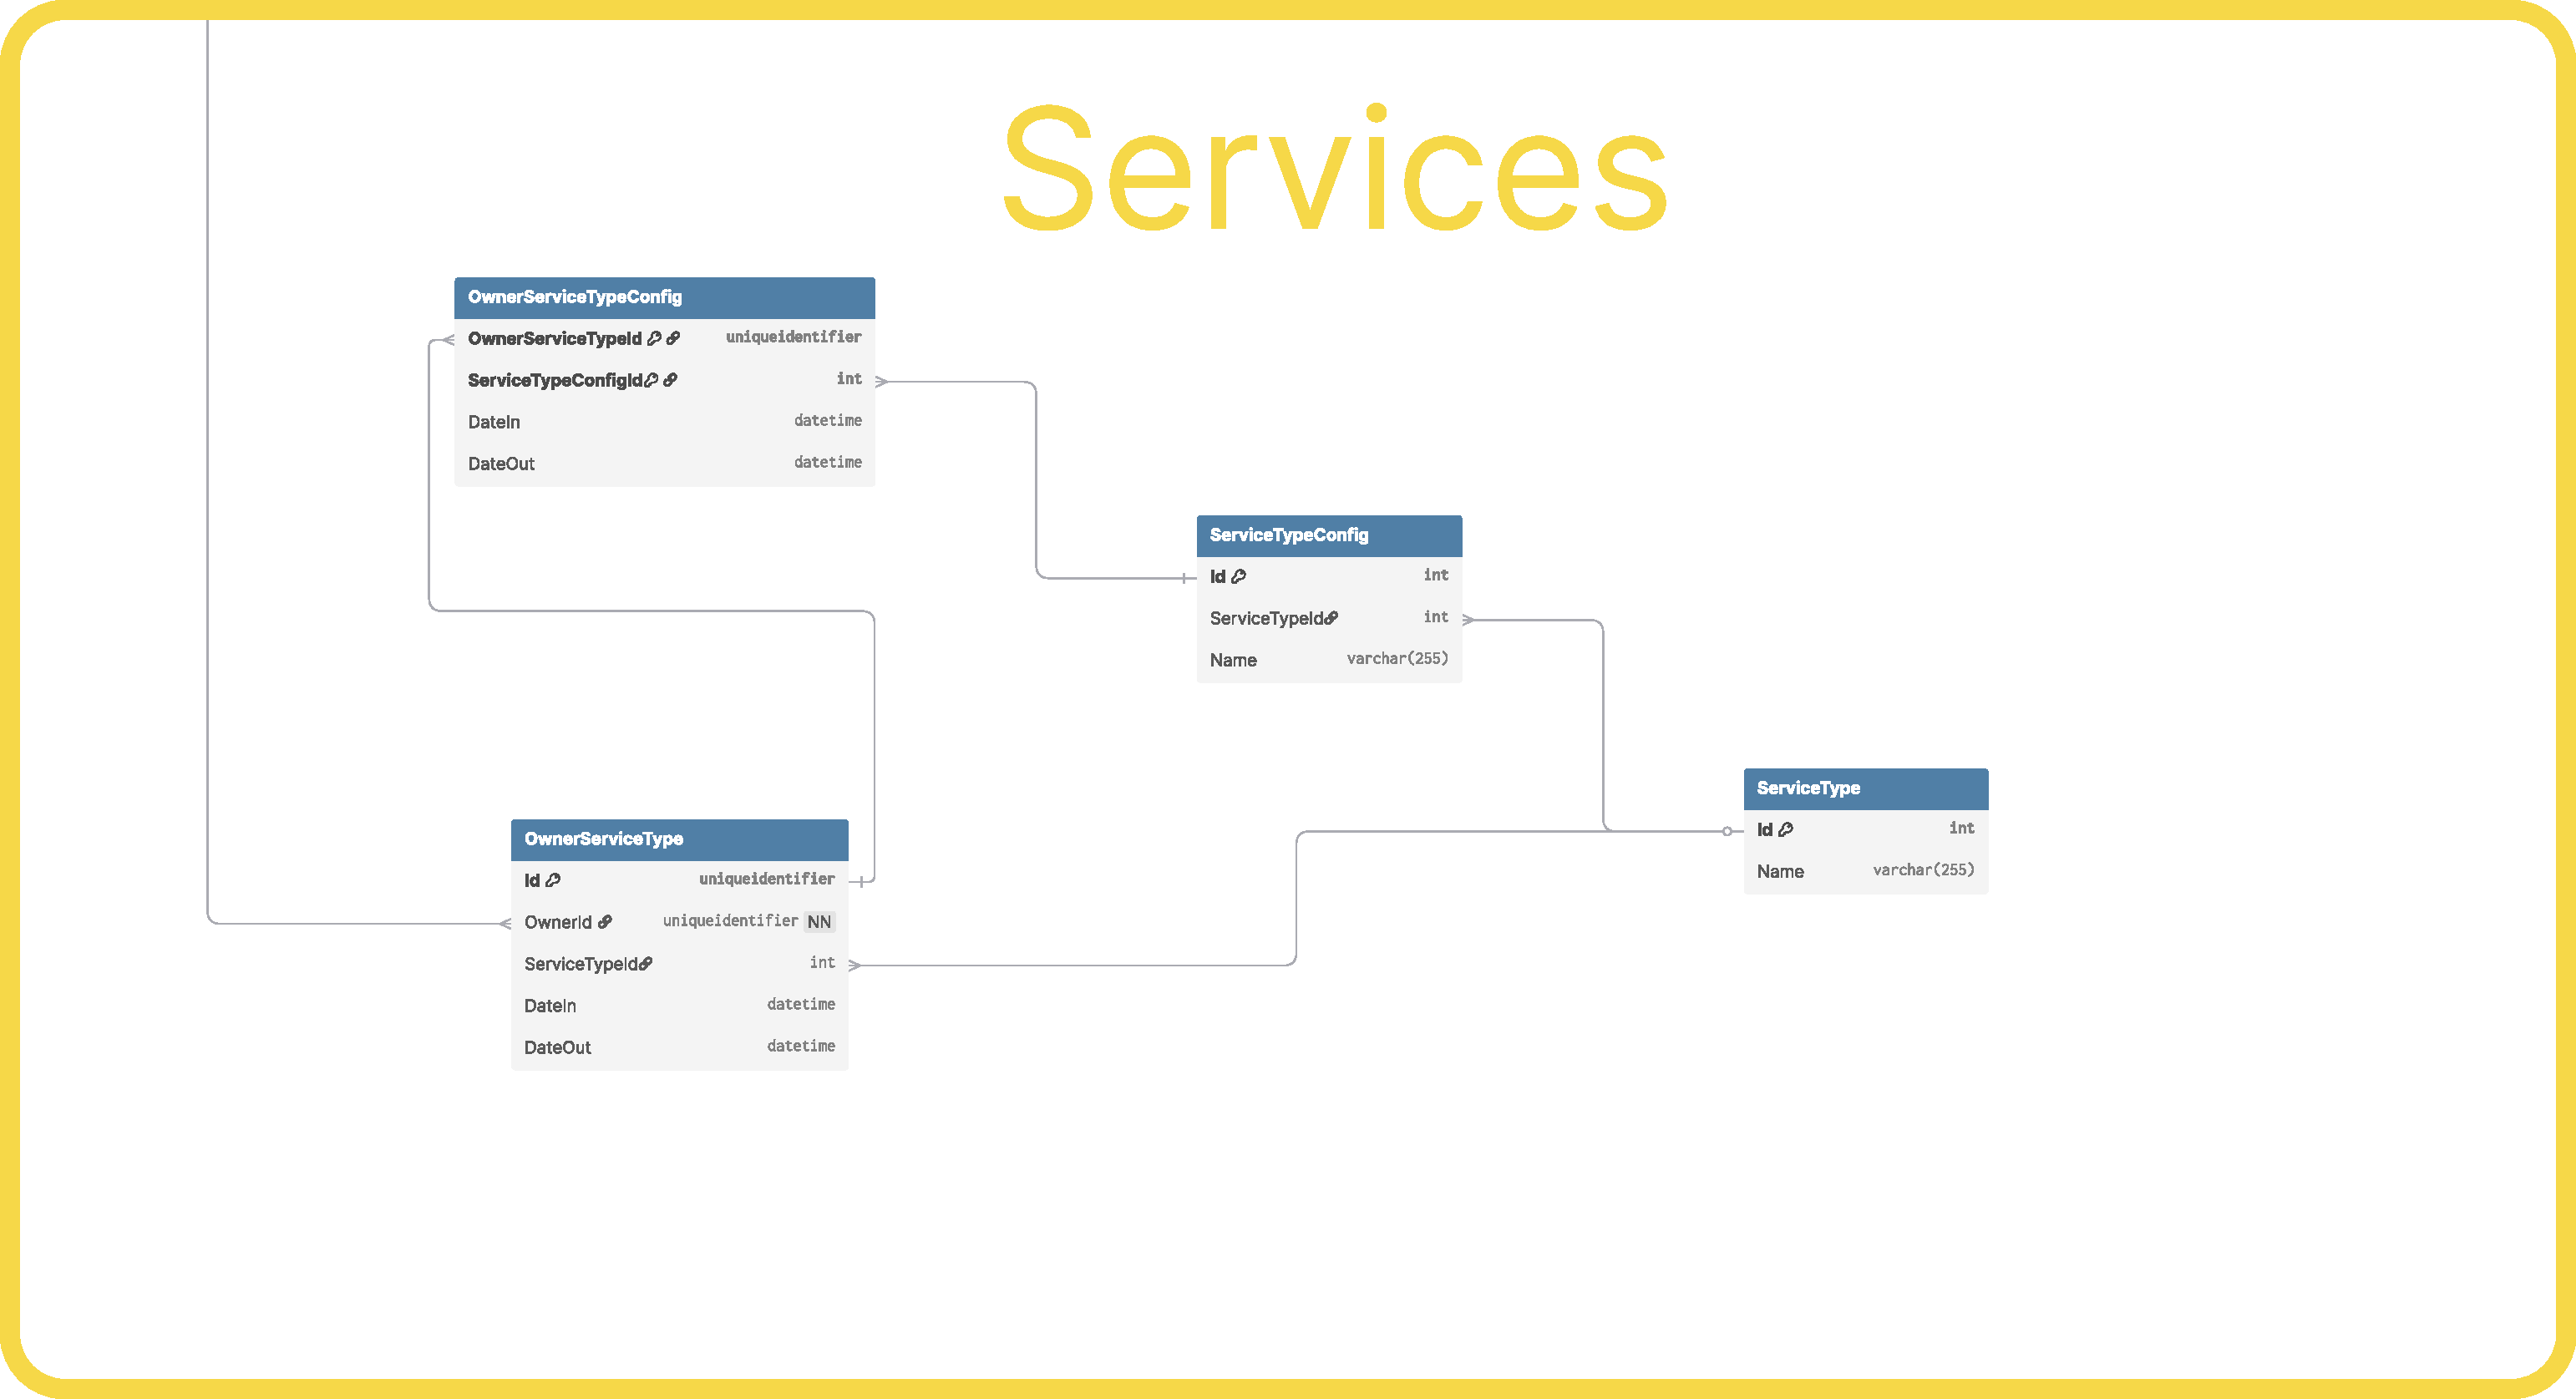
\includegraphics[width=\textwidth]{figs/dbDiagrams/Services}
  \label{fig:figure2}
\end{figure}

The services section starts with the tablke serviceType that has all type of services that exist, namely "bike sharing" and "Dealership"
This table has the following columns:
- Id, the identification of the service type
- name, the name of the service type

This table is connected with the Table Owner through the table OwnerServiceType.
This table has the info of the duration of the service to the owner.
It has the following columns:
- Id, the id of the owner service connection
- OwnerId, the identification of the owner
- ServiceType, the identification of the type of service is connected to the owner
- DateIn, the date when the service started
- DateOut, the date when the service ended

The serviceType is also connected with the table serviceTypeConfig that has the information of the various configuration of the dealership, like if does tasks division and assignment or in the evaluation it does the maintenance of the vehicle and identifies the tasks done.
It has the following columns:
- Id, the identification of the configuration
- ServiceTypeId, the identification of the service type is associated with
- Name, the name of the configuration

This table is associated with the OwnerServiceType in the table OwnerServiceTypeConfig since the dealership can chose which configuration it decides to have.
It has the following columns:
- OwnerServiceTypeId, the identification the connection of the service type and the dealership
- ServiceTypeConfigId, the identification of the configuration of the service type
- DateIn, the date when dealership start using the configuration started
- DateOut, the date when the dealership remove de configuration


\subsection{Vehicles and Owners} 


\begin{figure}[h]
  \caption{Database Vehicles and Owners diagram.}
  \centering
  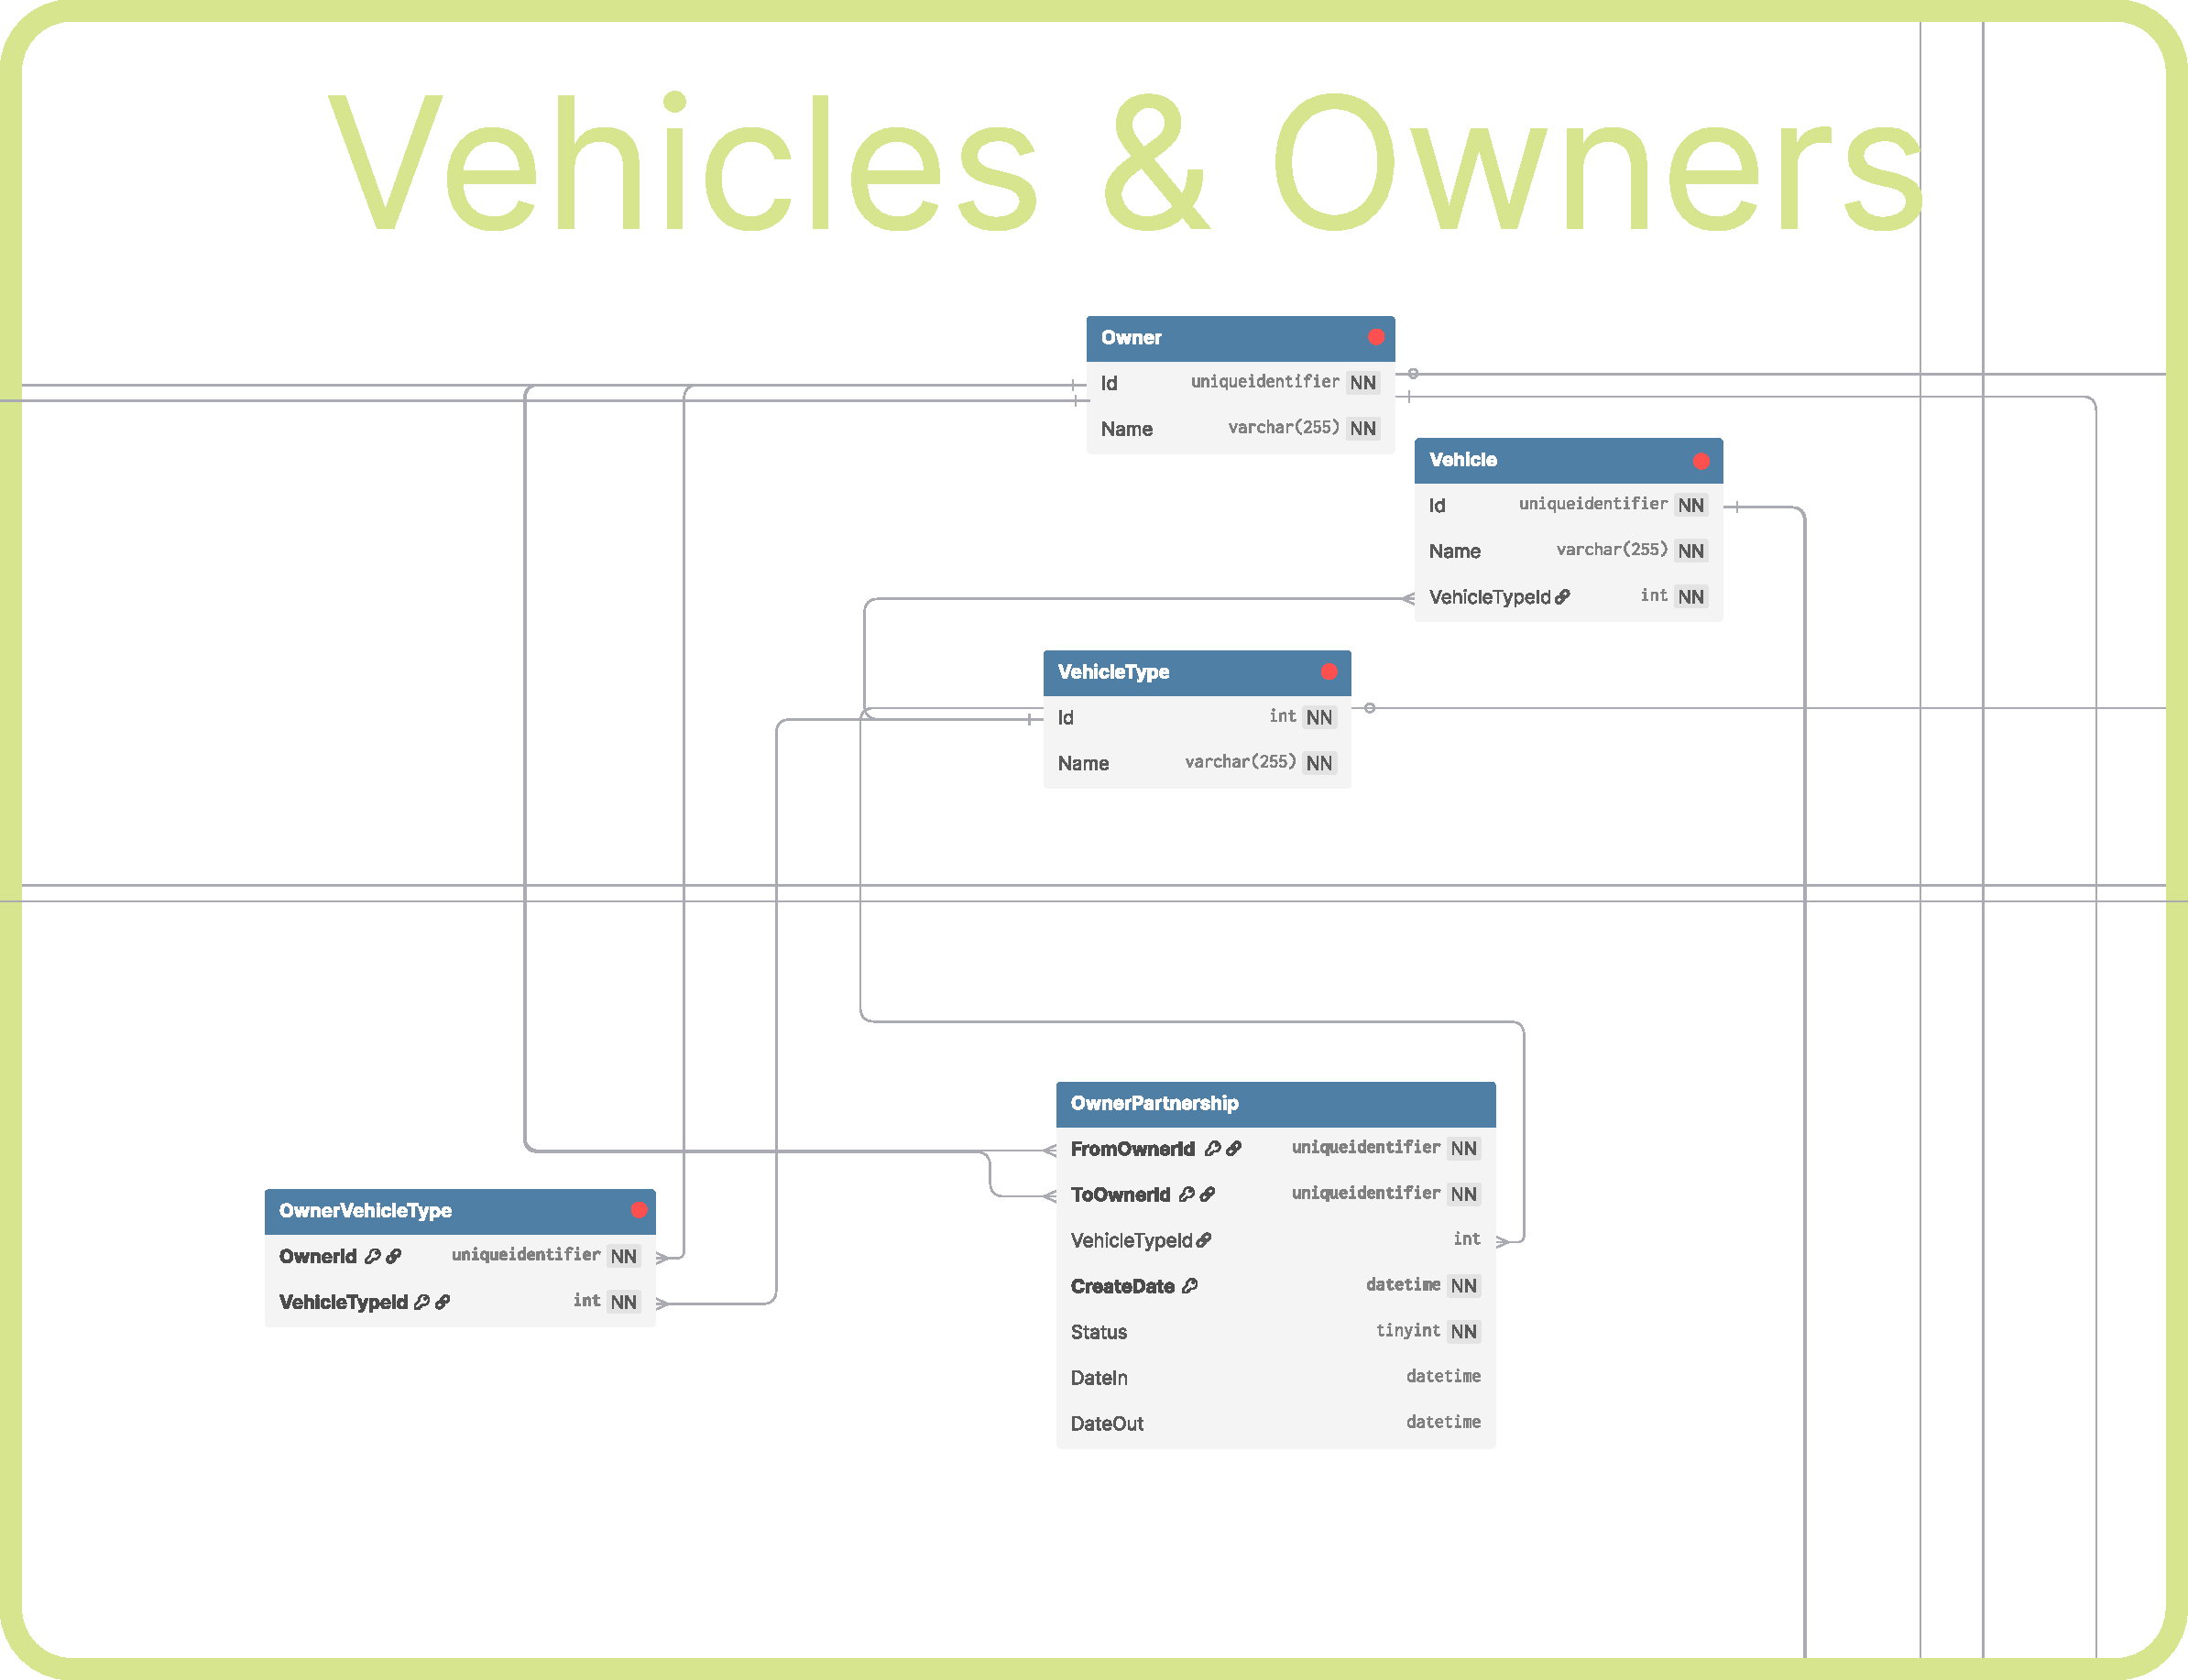
\includegraphics[width=\textwidth]{figs/dbDiagrams/Vehicles_and_Owners}
  \label{fig:figure2}
\end{figure}


This section the tables Owner, Vehicle and VehicleType already existed in the lightmobie database.
The Owner table registers the information of the dealerships and bike sharing entities.
The vehicle table registers the information of each vehicle and is connected with the vehicleType thar stores the type of vehicles, like "Eletric bikes", "convention bikes", etc.

I created the table OwnerVehicleType to allow disinguish between dealership availability to do a maintenance to specific type of vehicles. This table only has the column of connection of the two tables, owner and vehicleType.
The OwnerPartnership table is used to allow bikesharing entities to share information with dealership for it to do the maintenance. If a dealership is not connected to a bike sharing entity is not allowed to view theres vehicle information.
This table has the following columns:
- FromOwnerId, the identification of the bike sharing entity that wants to associate with the dealership
- ToOwnerId, the identification of the dealership that is requested to do maintenances to the bikesharing entity
- VehicleTypeId, the identification of the type of vehicles the bike sharing entity wants the dealership to do maintenances
- CreateDate, the date the request was created
- Status, the satus of the request, it can be Request, the request is waiting for response from the dealership; Accept, the request was accepted; Denied, the request was denied


\section{Implementation}

\subsection{Rececionist view}
The rececionist application view has only one page seen in \ref .

\begin{figure}[h]
  \caption{Rececionist home page.}
  \centering
  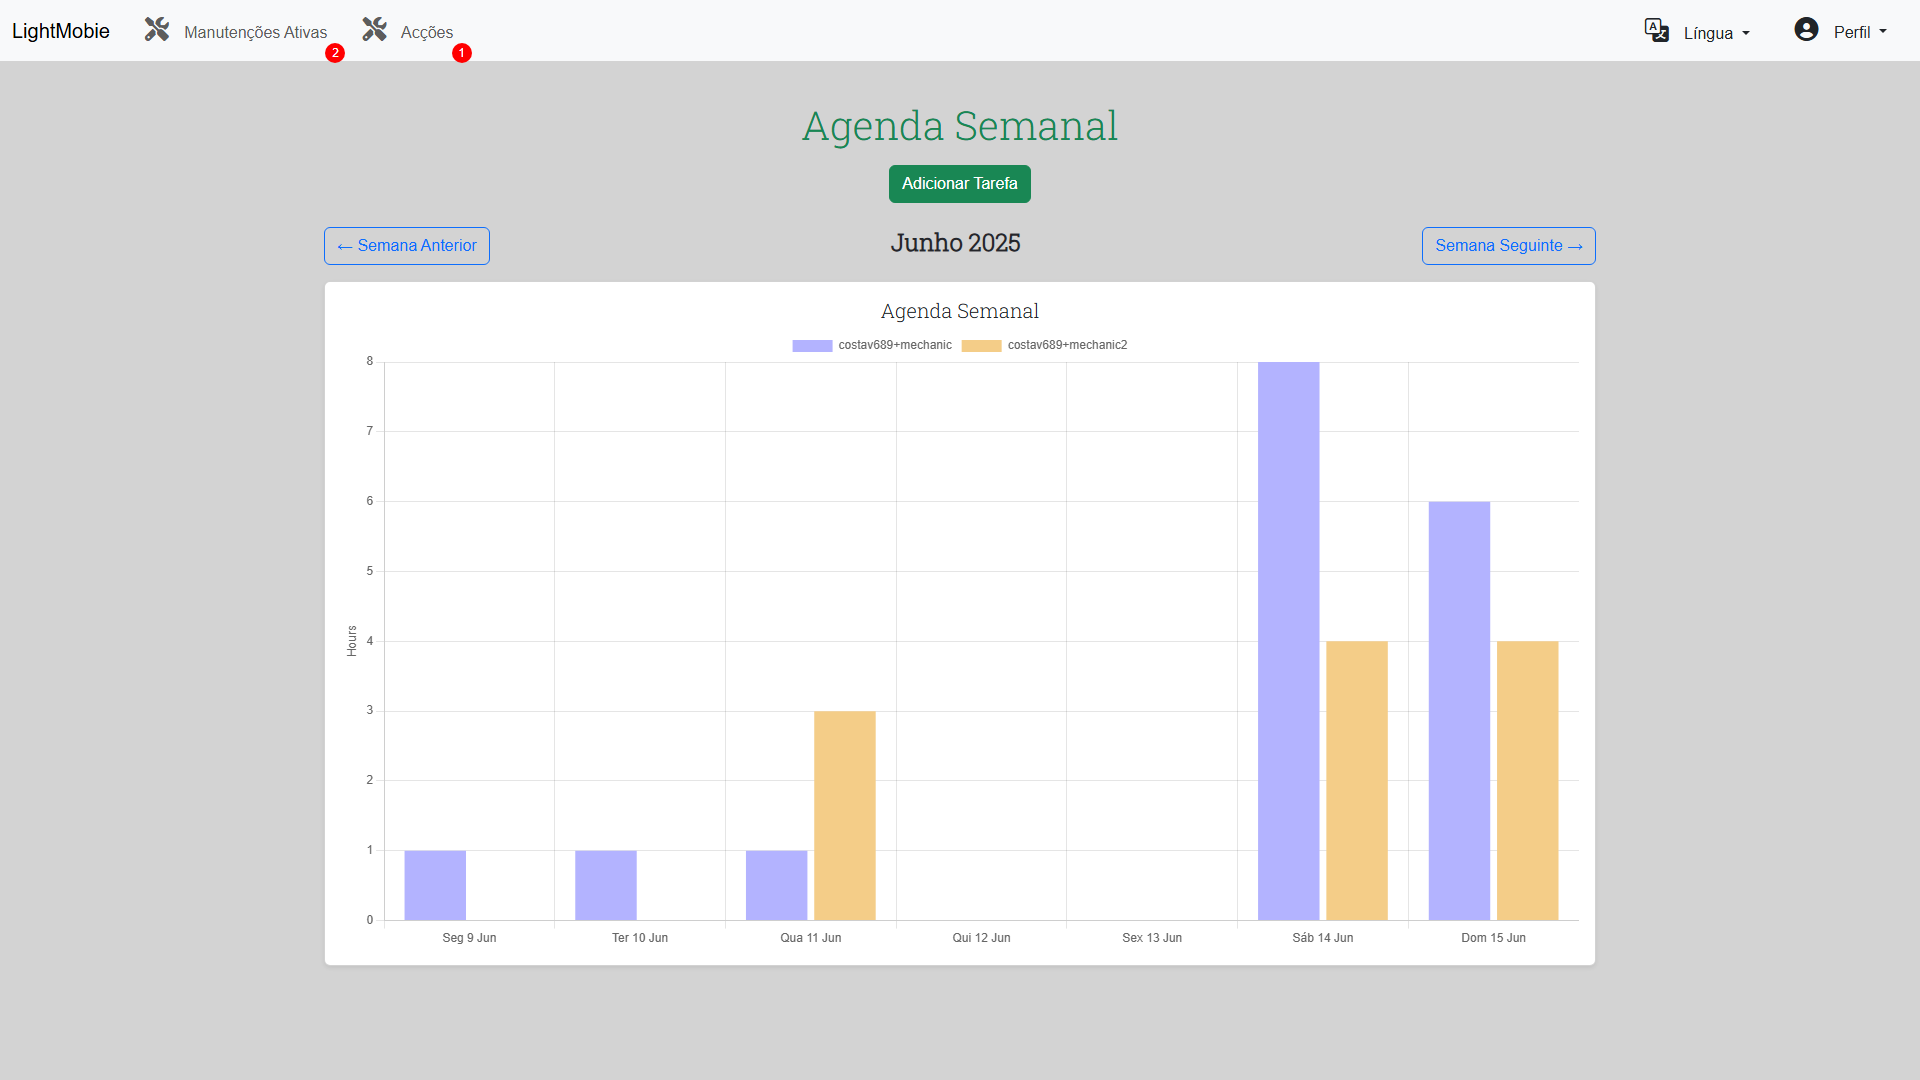
\includegraphics[width=\textwidth]{figs/Implementation/rececionist/rececionistHomePage}
  \label{fig:figure2}
\end{figure}

In this page it is visible a bar chart with the expected working hours of each mechanic for the days of the selected week.
The mechanic can navegate through out the year using the buttons "próxima semana" e "semana anterior" to go to the next and previous week respectively.
This information is relevant to understand which mechanic is available to do a vehicle evaluation and accomplish the Use Case 1.1 – Maintenance Schedule.
To schedule a maintenance a rececionist has two options: click on the green button "Adicionar Tarefa" or click on the graph on the specific date he wants to choose.
Both options will open up a modal seen in figure \ref.

\begin{figure}[h]
  \caption{Rececionist schedule maintenance.}
  \centering
  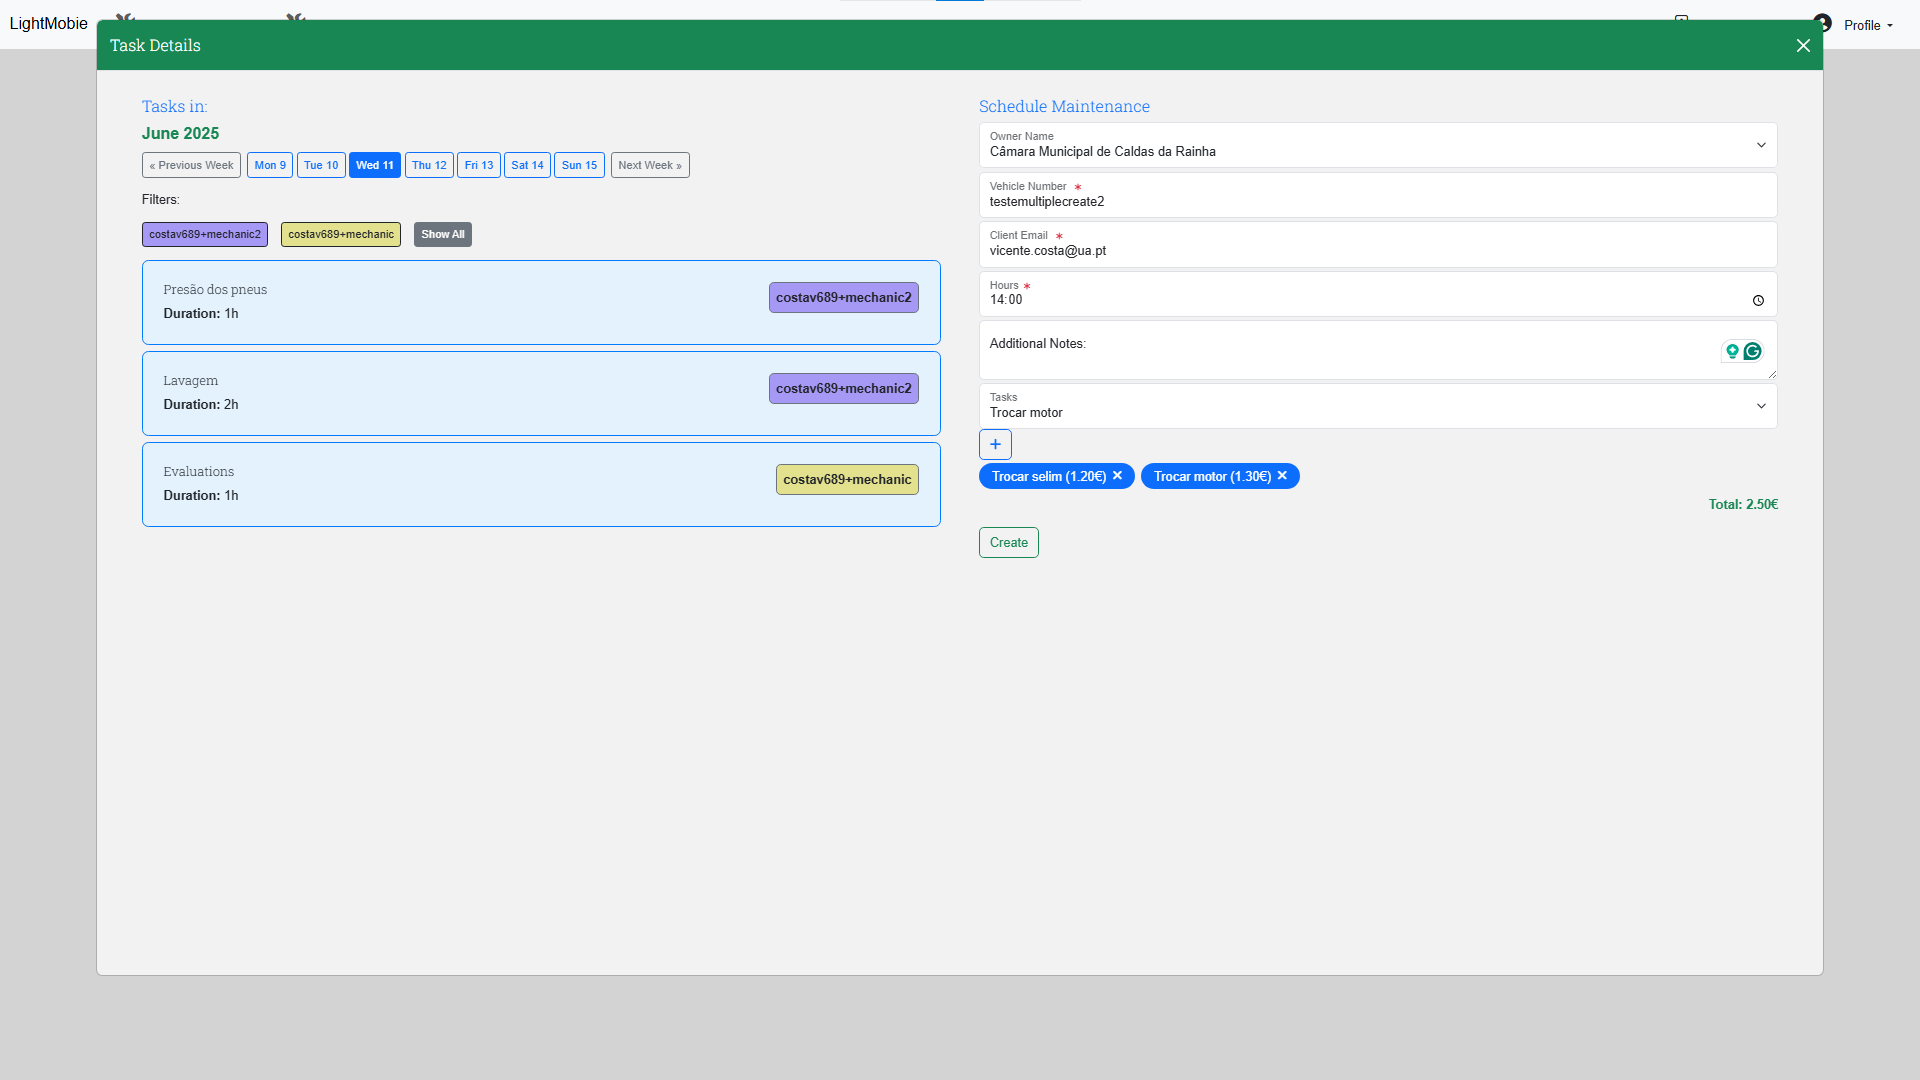
\includegraphics[width=\textwidth]{figs/Implementation/rececionist/addTask}
  \label{fig:figure2}
\end{figure}

In the modal, the rececionist can still change the date of the maintenance in the top lef corner and it will show the tasks of the mechanics of that date, including the name of the task and the expected time to complete that task.
To finish the schedule of the maintenance, the rececionist must fill the form on the right side of the modal.
The options are:
- The name of the entity: it is optional and it is refers to a bikesharing entity that has a partnership relational with the dealership;
- the vehicle registration: it is mandatory and it refers to the vehicle registration of the vehicle, it only accepts vehicles from partner entities or from users without entity; this field has autocompletes
- the client email: it is mandatory and it refers email of the client, if the client doesn't exist it is created a new client for that account, and an email is sent to that user to finish the account creation;  if the user exist and is related to a partner entity or is a solo client, the email can be autocompleted;
- the hours of the vehicle arrival: it is mandatory and it refers to the agreed time when the client will bring the vehicle
- pre-selected tasks: it is optional and it refers to tasks that the rececionist may already add to the maintenance as the will of the client; it has a price tag below to indicate the expected price of the maintenance with those pre-selected tasks
- adicional notes: it is optional and it refers to notes that the rececionist may want to pass to the mechanic responsible for the vehicle evaluation
Finally the rececionist clicks on the button "Criar" to finish the maintenance shedule and complete the use case 1.1 – Maintenance Schedule.
%% Adicionar foto de mostrar o form de criar conta do user

\begin{figure}[h]
  \caption{List of active maintenances.}
  \centering
  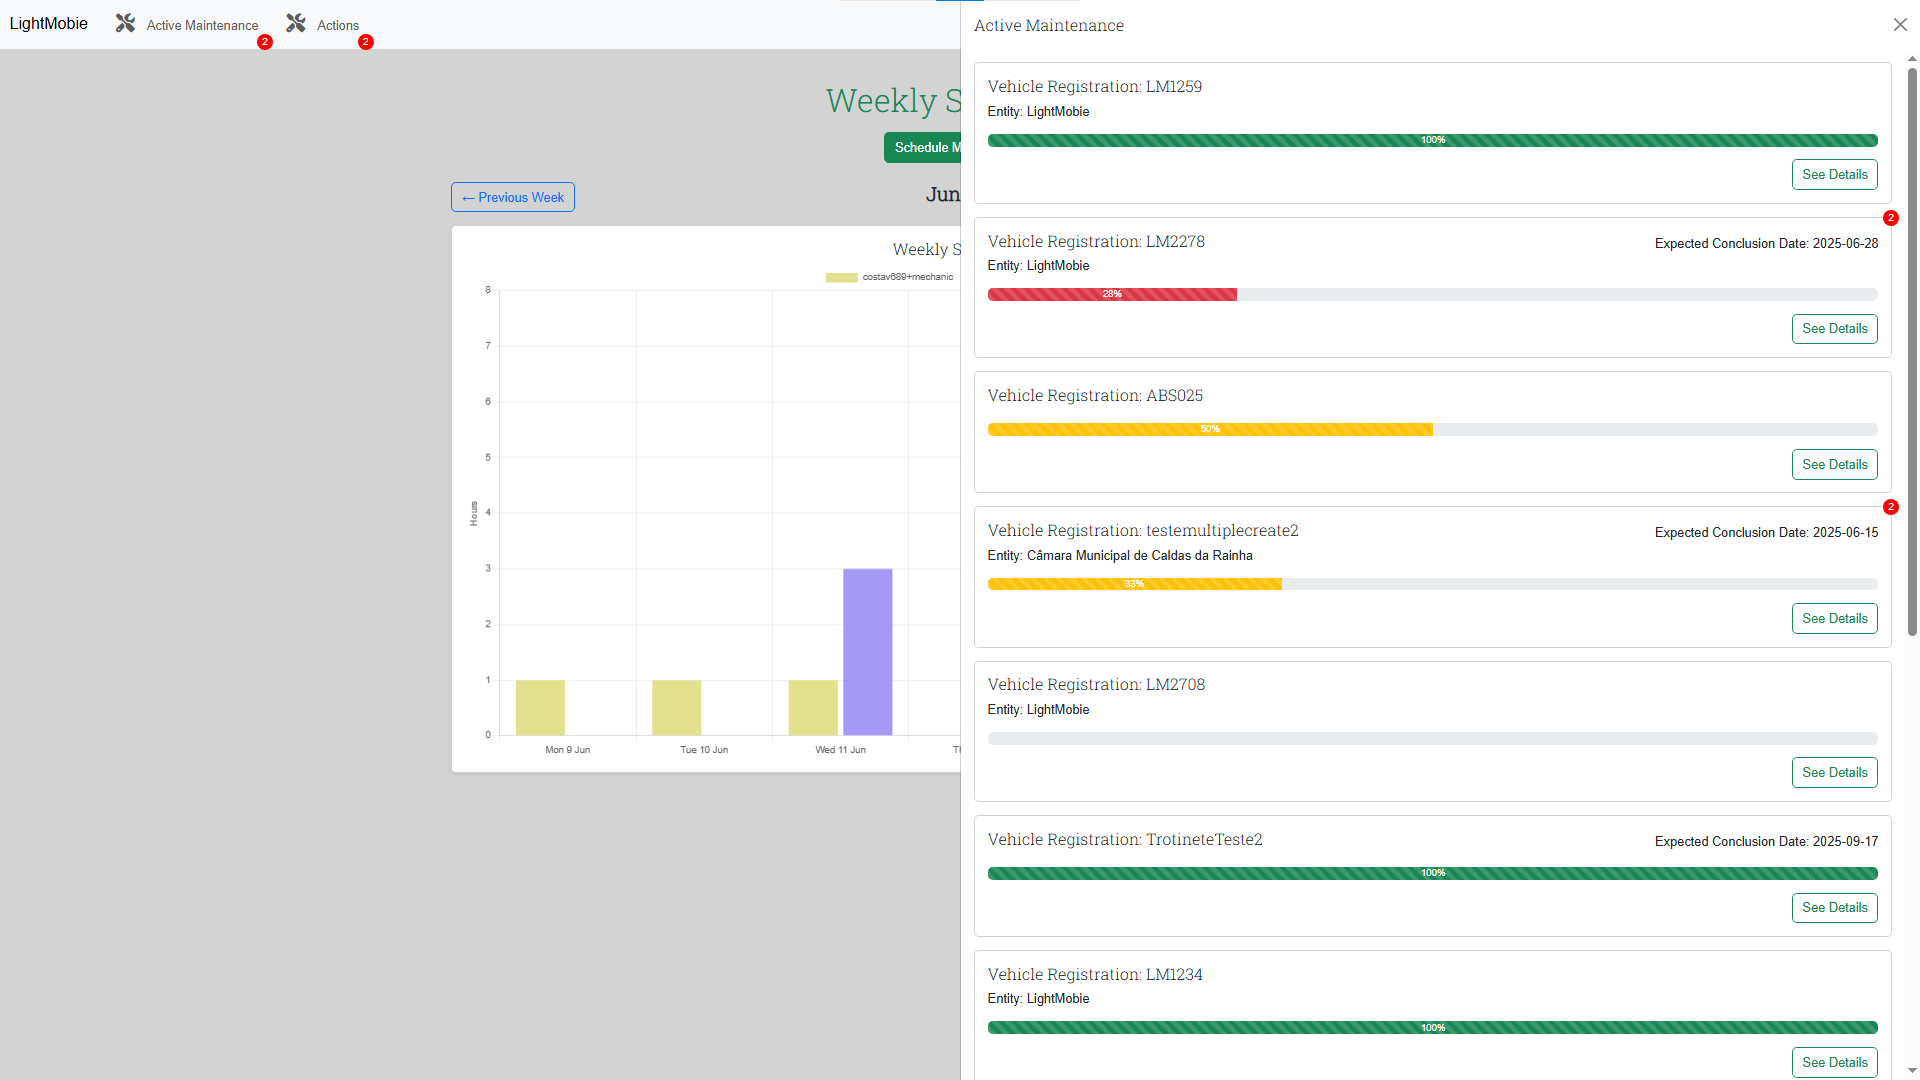
\includegraphics[width=\textwidth]{figs/Implementation/rececionist/activeMaintenances}
  \label{fig:figure2}
\end{figure}

When clicking on the button "Manutenções Ativas" on the menu it shows an offcanvas with the list of non finished maintenances, as seen in \ref.
This button can have a red circle with a number that represents the number of maintenances that has a maintenance change and needs the rececionist to contact the client.
In the offcanvas, each card has the information to identify the maintenance and indicate the progress, namely:
- the vehicle registration: the registration number of the vehicle that is doing the maintenance
- the entity: the name of the entity of the vehicle
- the expected conclusion date: the expected date to conclude the maintenance
- the progress of the maintenance: the percentage of tasks completed
In each maintenance card may be seen a red circle in the top right corner with a number. 
This represents the number of maintenance changes for that maintenance, like, for example a task is delayed and another has a part change suggestion.

\begin{figure}[h]
  \caption{Active maintenance details Information tab.}
  \centering
  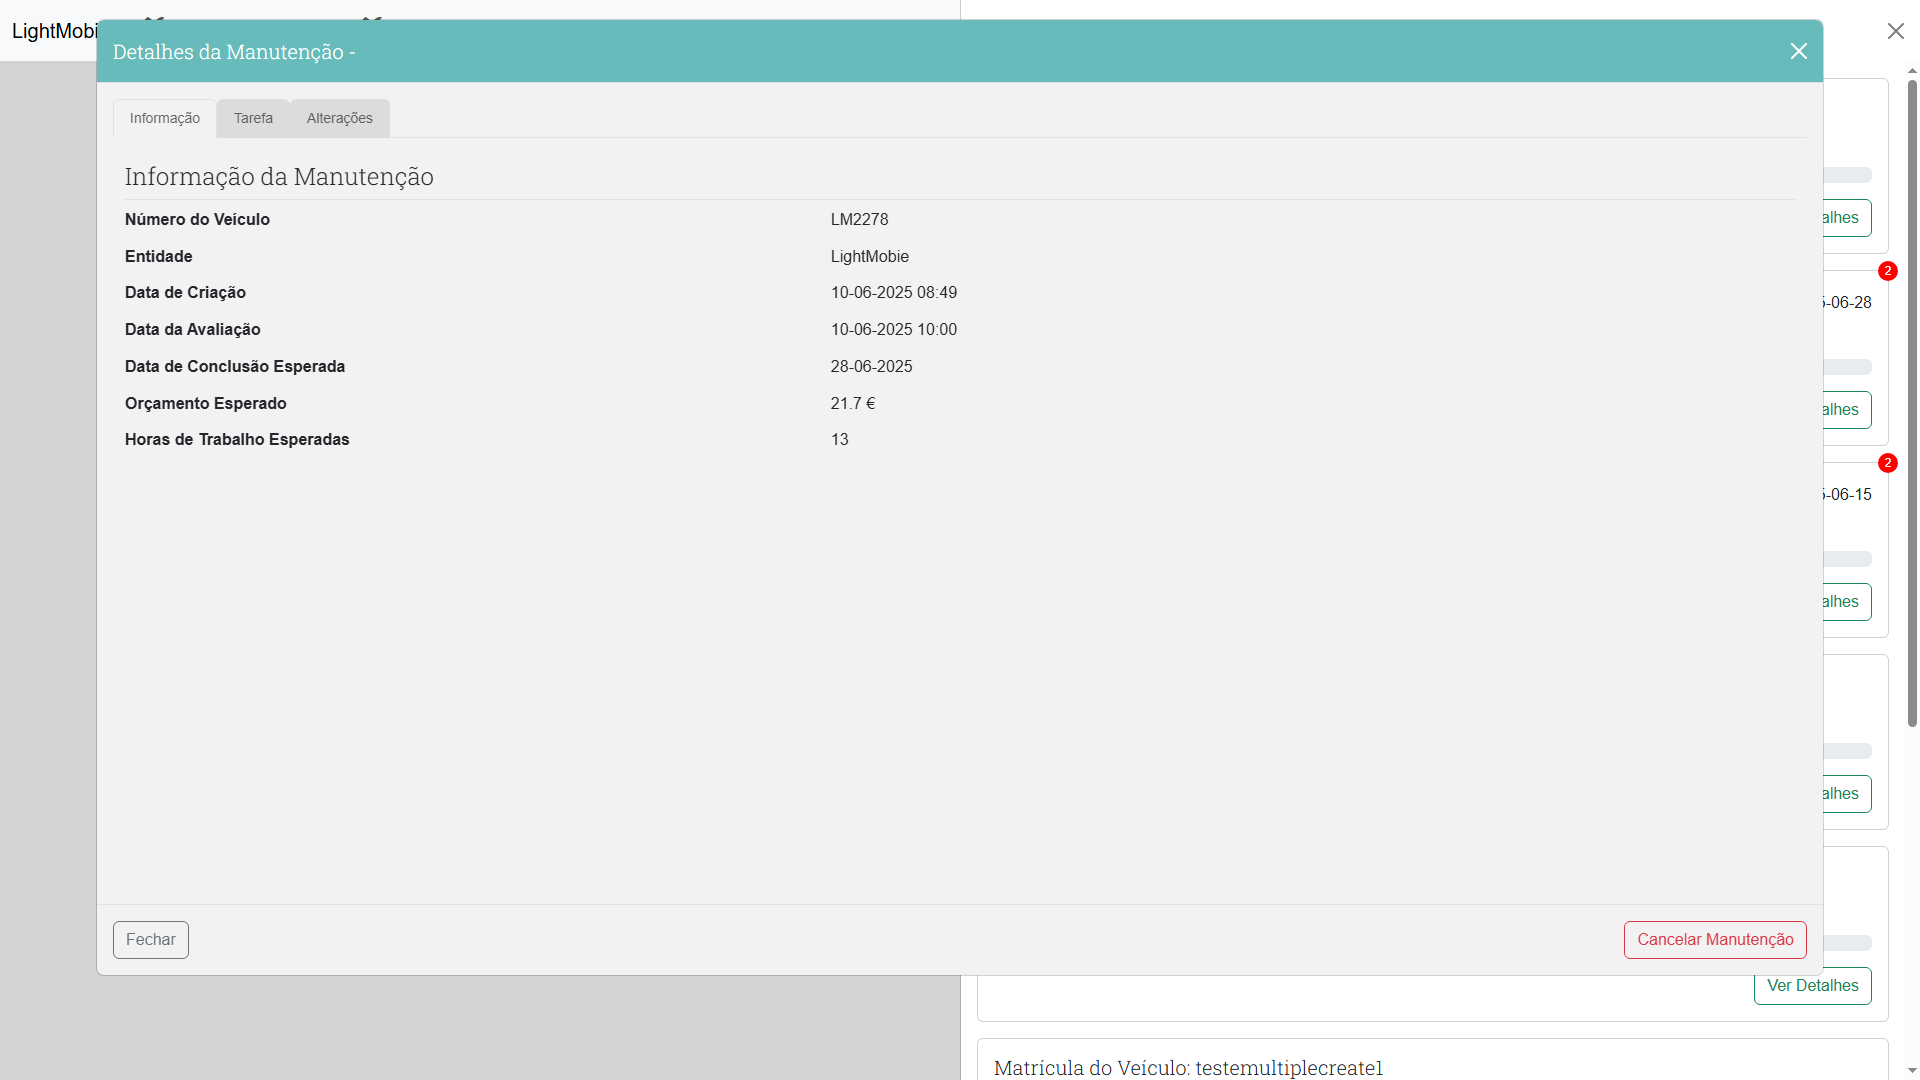
\includegraphics[width=\textwidth]{figs/Implementation/rececionist/maintenance_details}
  \label{fig:figure2}
\end{figure}


When clicking on "Ver Detalhes" of a maintenance it opens a modal as seen in the figure \ref.
In this modal has the information that the rececionist may need to answer the client if the client calls to ask for it.
With this the Use Case 1.3 – Collect information about a maintenance request is completed.
The information shared in the modal, namely in the "Information" tab is:
- Vehicle registration
- Entity name
- Creation date of the maintenance
- Evaluation date of the vehicle
- Expected conclusion date
- Expected budget
- Expected Working Hours 

\begin{figure}[h]
  \caption{Active maintenance details task tab.}
  \centering
  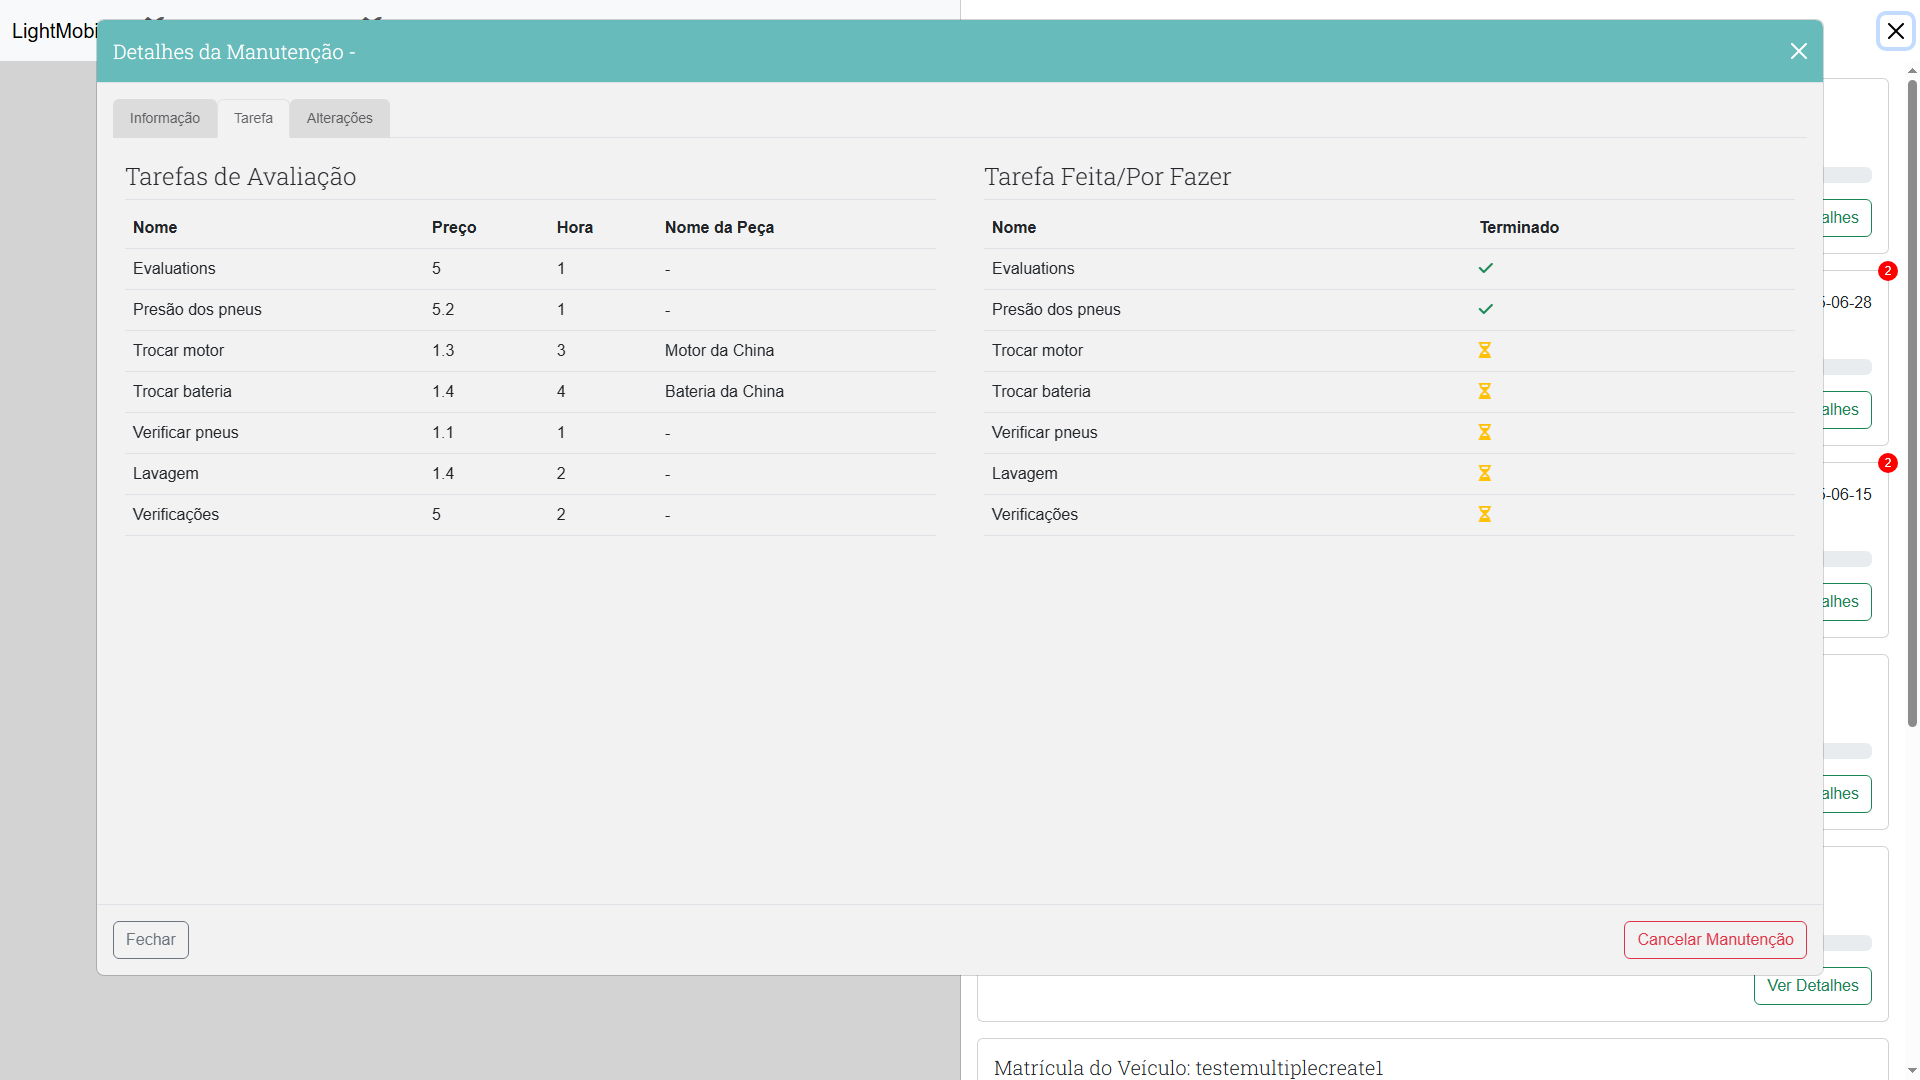
\includegraphics[width=\textwidth]{figs/Implementation/rececionist/maintenance_details_task}
  \label{fig:figure2}
\end{figure}

When navigating to the "Tarefa" tab it shows the tasks selected by the evaluation on the left side and the status of the task on the right side.
On the left side, for each task it shows:
- the price 
- the number of hours to complete
- the name of the part to complete the task
On the right side, for each task shows the status that can be:
- Invalid, represented as a red cross
- completed, represented as a green check 
- waiting to be completed, represented as a yellow Hourglass
I decided to simply to this three states since the client doesn't need to understand the full flow of a task.


\begin{figure}[h]
  \caption{Active maintenance details change tab.}
  \centering
  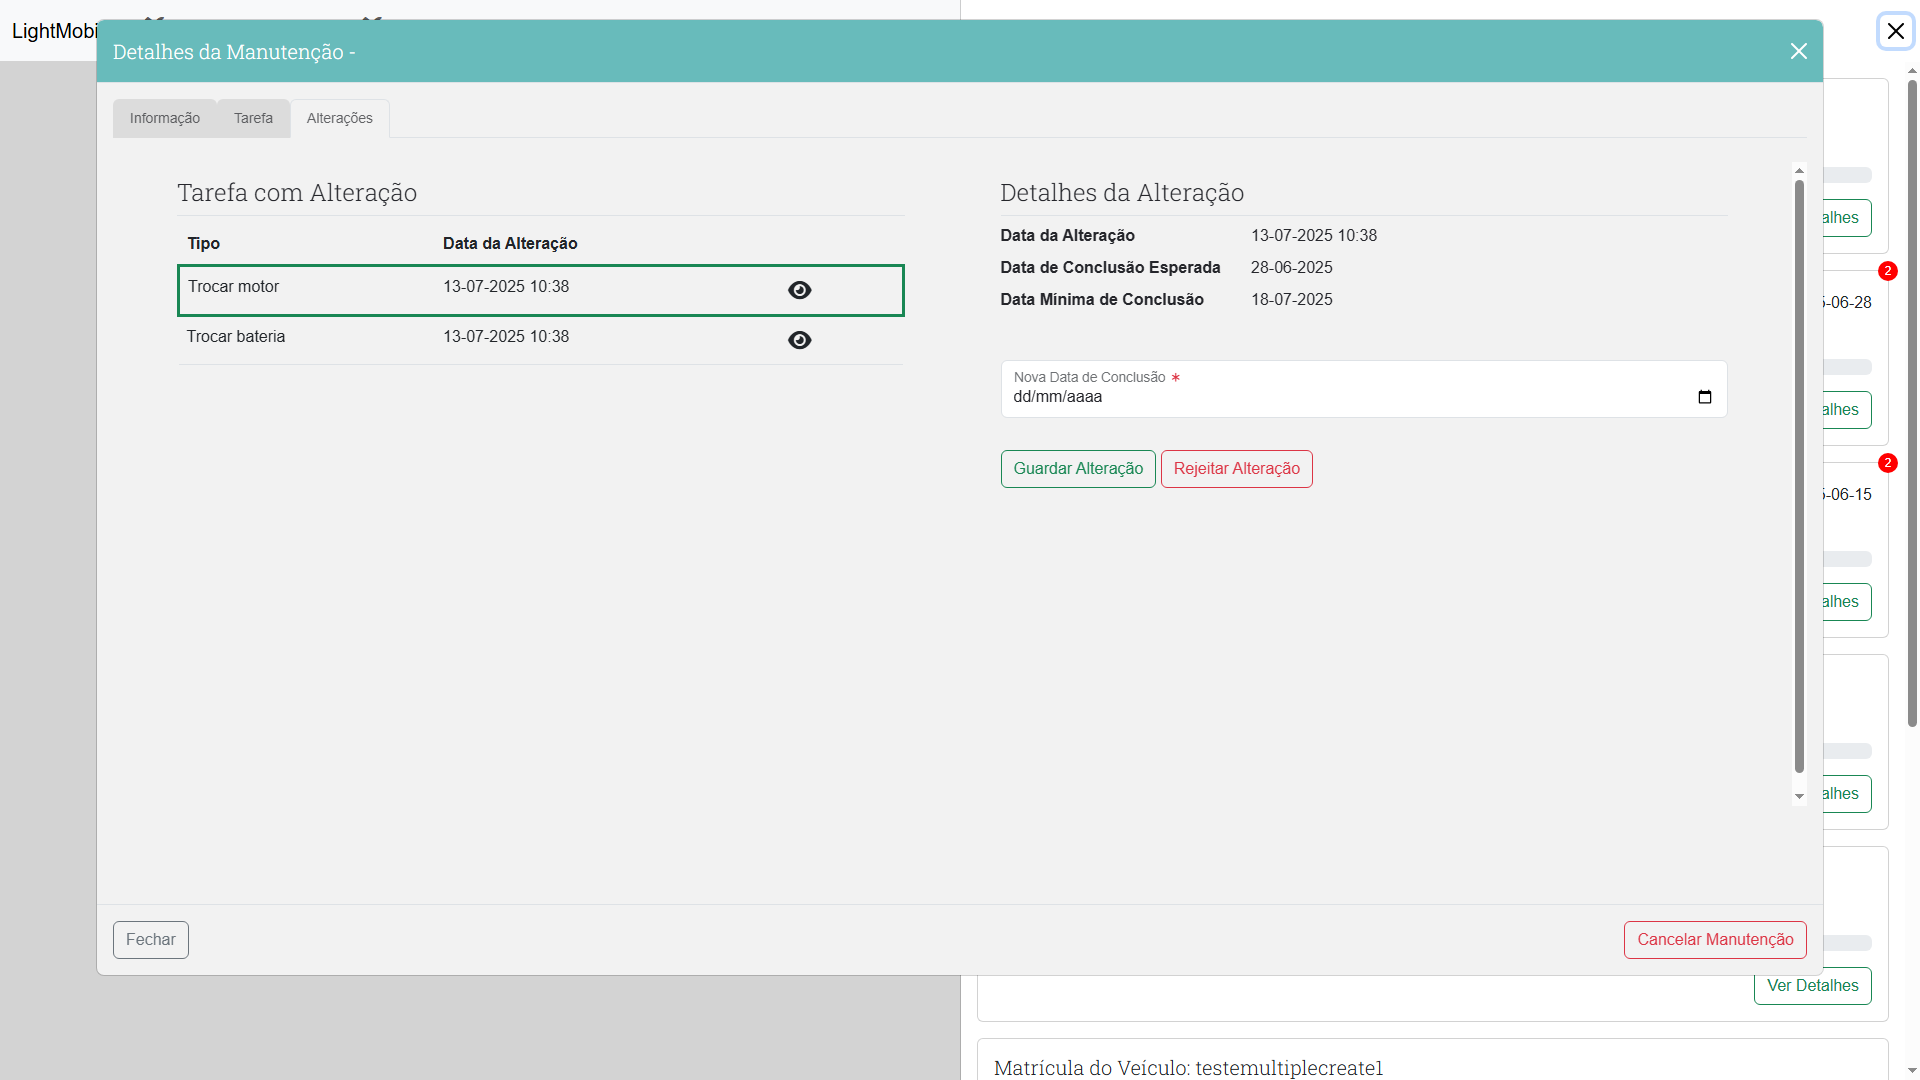
\includegraphics[width=\textwidth]{figs/Implementation/rececionist/maintenance_details_change}
  \label{fig:figure2}
\end{figure}

The last tab of the modal is "Alterações" that show the maintenance changes of the maintenance.
As we can see in \ref it shows all the maintenance changes in the left side with the information of the task that provoked the change and the change date.
And the change details on the right. This details show the following information:
- the date of the change
- the expected conclusion date of the maintenance
- the new vehicle part of the change
- and the new minimum expeceted conclusion date

In this scenario the rececionist may click on the button "Guardar alteração" to agree to the changes or "Rejeitar Alteração" and,since this maintenance change has a minimum conclusion date, will invalidate the task that since it is delayed.
With this the Use Case 1.4 – Accept maintenance changes and the Use Case 1.5 – Refuse maintenance changes are completed.

In the modal is also possible to accomplish the Use Case 1.7 – Cancel Maintenance by clicking in the button "Cancelar Manutenção" in the bottom right corner of the modal, as seen in \ref .
Also, in the same location, if all the tasks are completed, it show a button call "Conluir Manutenção" that allows the Use Case 1.6 – Vehicle Delivery.


\begin{figure}[h]
  \caption{List of maintenances that the evaluation is finished and need to comunicate with the client to decide wich task to be done.}
  \centering
  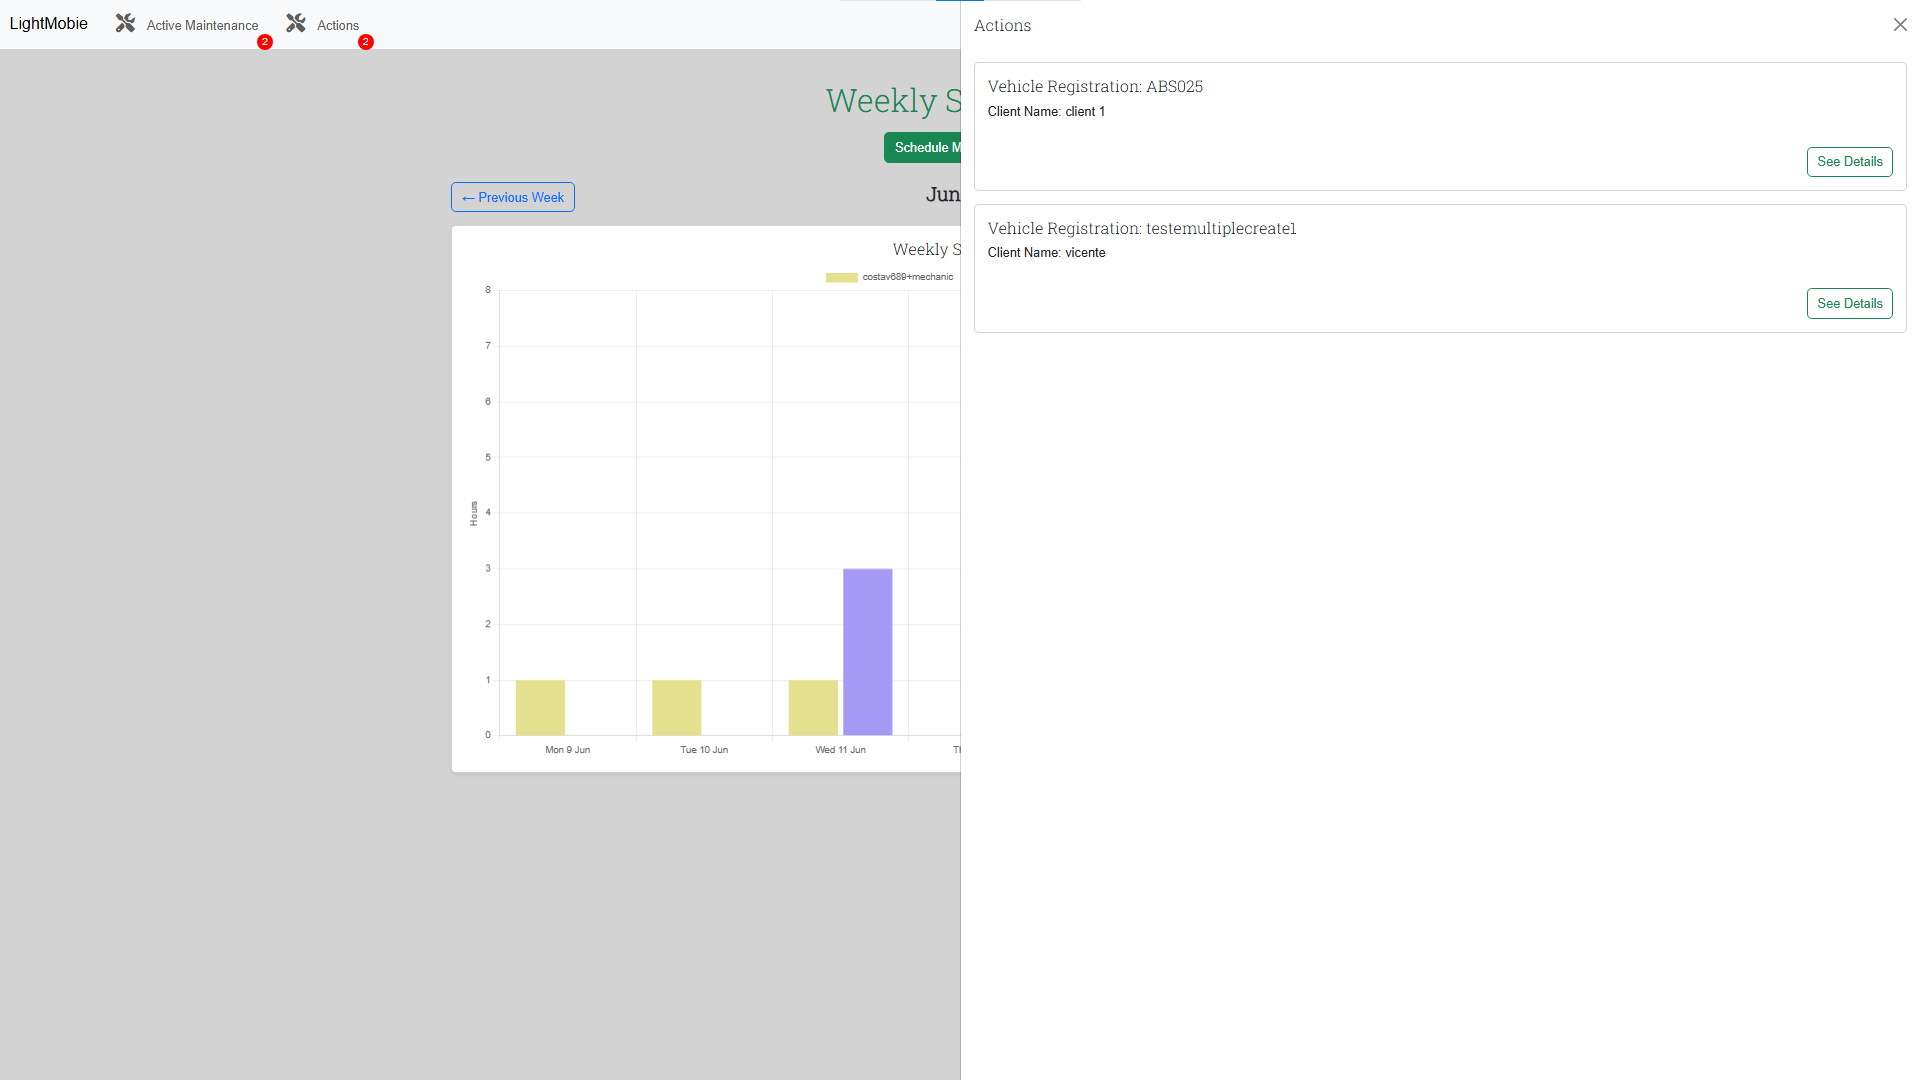
\includegraphics[width=\textwidth]{figs/Implementation/rececionist/action_list}
  \label{fig:figure2}
\end{figure}


The last button of the menu is the "Acções" button, this button, when clicked, shows a list of maintenances where the vehicle evaluation just finished and it needs the client to comfirm wich task needs he agreeds to be done.
Each maintenance is represented as a card, as seen in \ref with the vehicle registration and the client name or entity name.

\begin{figure}[h]
  \caption{Maintenance action details.}
  \centering
  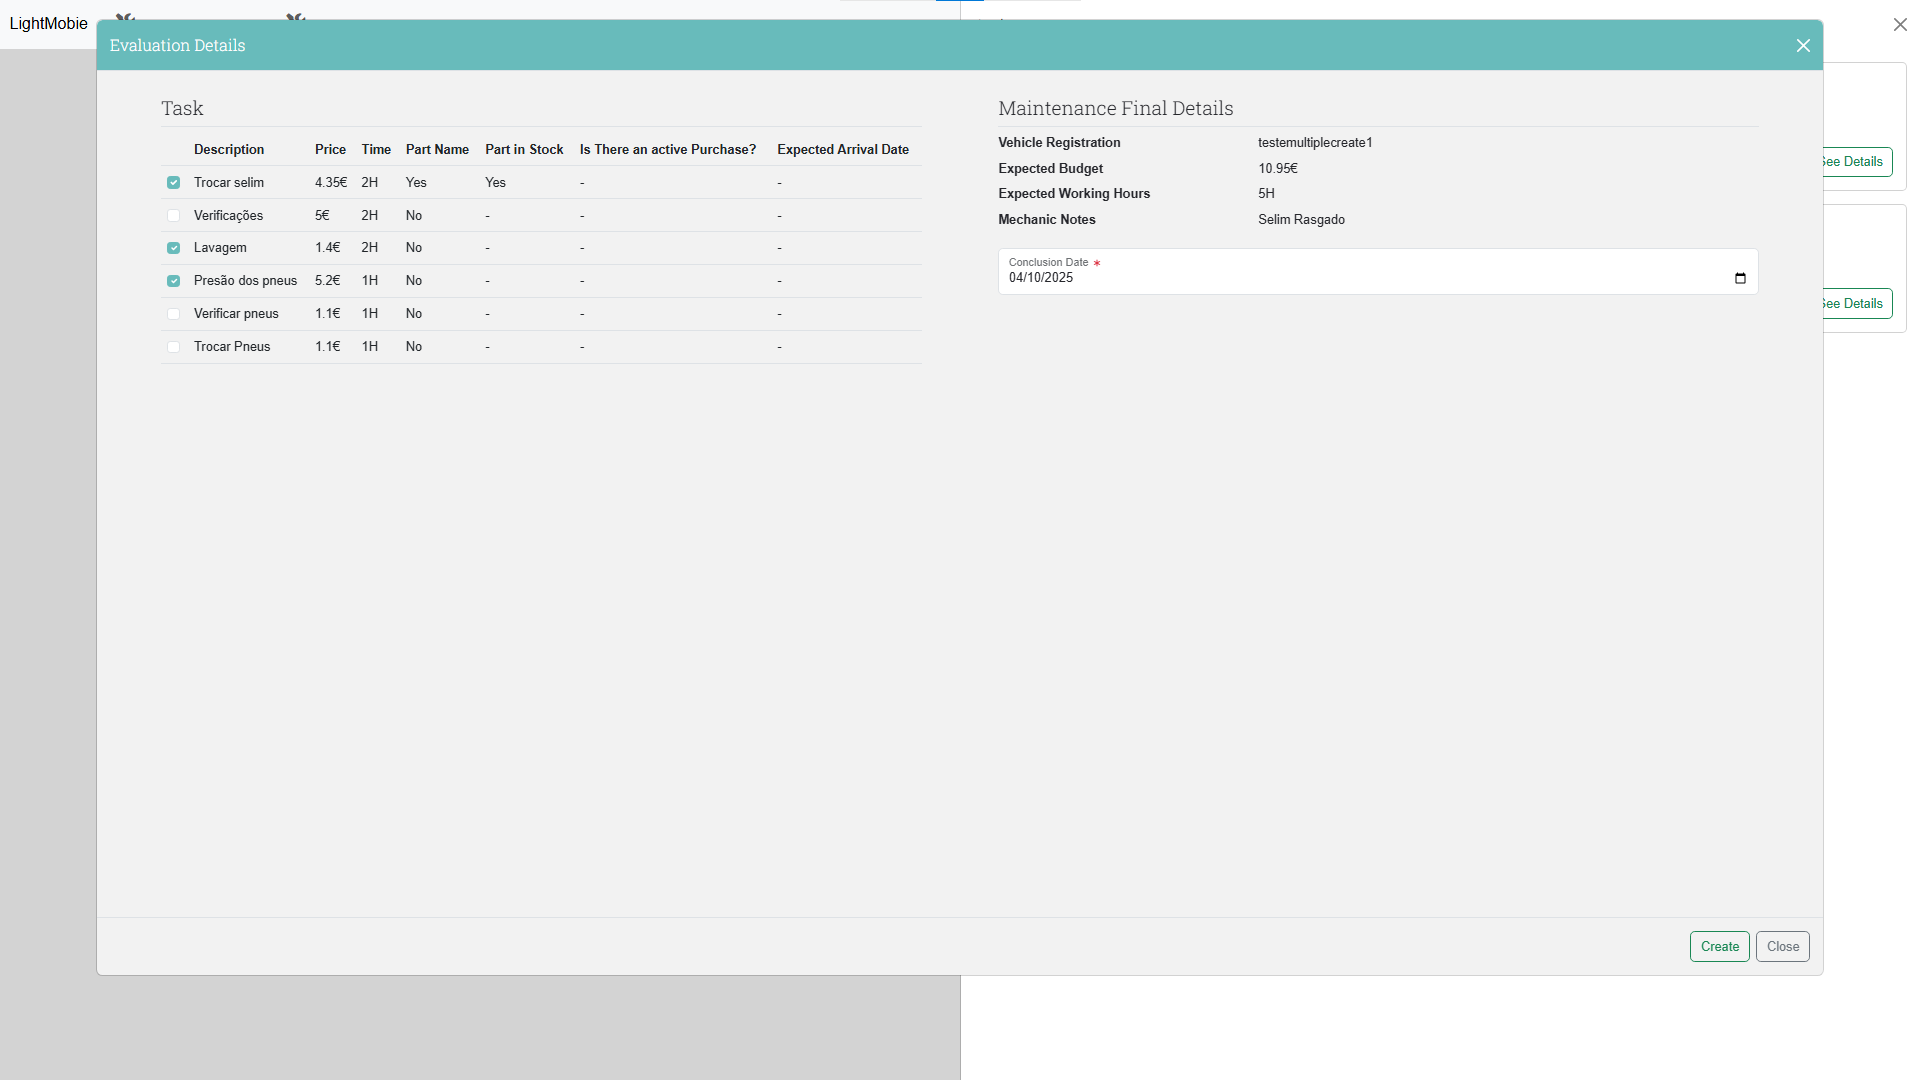
\includegraphics[width=\textwidth]{figs/Implementation/rececionist/action_details}
  \label{fig:figure2}
\end{figure}

When clicking on the button "Ver Detalhes" on a maintenance card, it shows a modal as sen in \ref.
In this modal, the Use Case 1.2 – Define maintenance details is addressed where it is showned a list of the tasks that the mechanic selected with the following information:
- name of the task
- the price of the task
- the number of hours to complete the task
- If it needs to change the part
- If the part is in stock on the warehouse
- There is already an active purchase for that part if the part is not in stock
- The expected data of the arrival of the part if the part is not in stock

On the right side of the modal, it is showend the vehicle registration, the expected budget, that changes with the task being selected; the expected working hours, that also changes with the selection of the tasks; and the evaluatiuon Mechanic notes.
To complete the maintenance the rececionist choses the tasks the client wants to be done and selects a appropriate date for the conclusion date and clicks on the button "Criar" on the bottom right corner.

If the rececionist would like to change the language it can do it on the right corner of the menu, the application handles portuguese and english. If he would like to leave, he can click on the button profile on the right of the language button and click "Terminar sessão".


\subsection{Mechanic view}

The mechanic application layout structure is very similar as the rececionist as seen in \ref and in \ref.

\begin{figure}[h]
  \caption{Mechanic home page with simple, late and previous started task.}
  \centering
  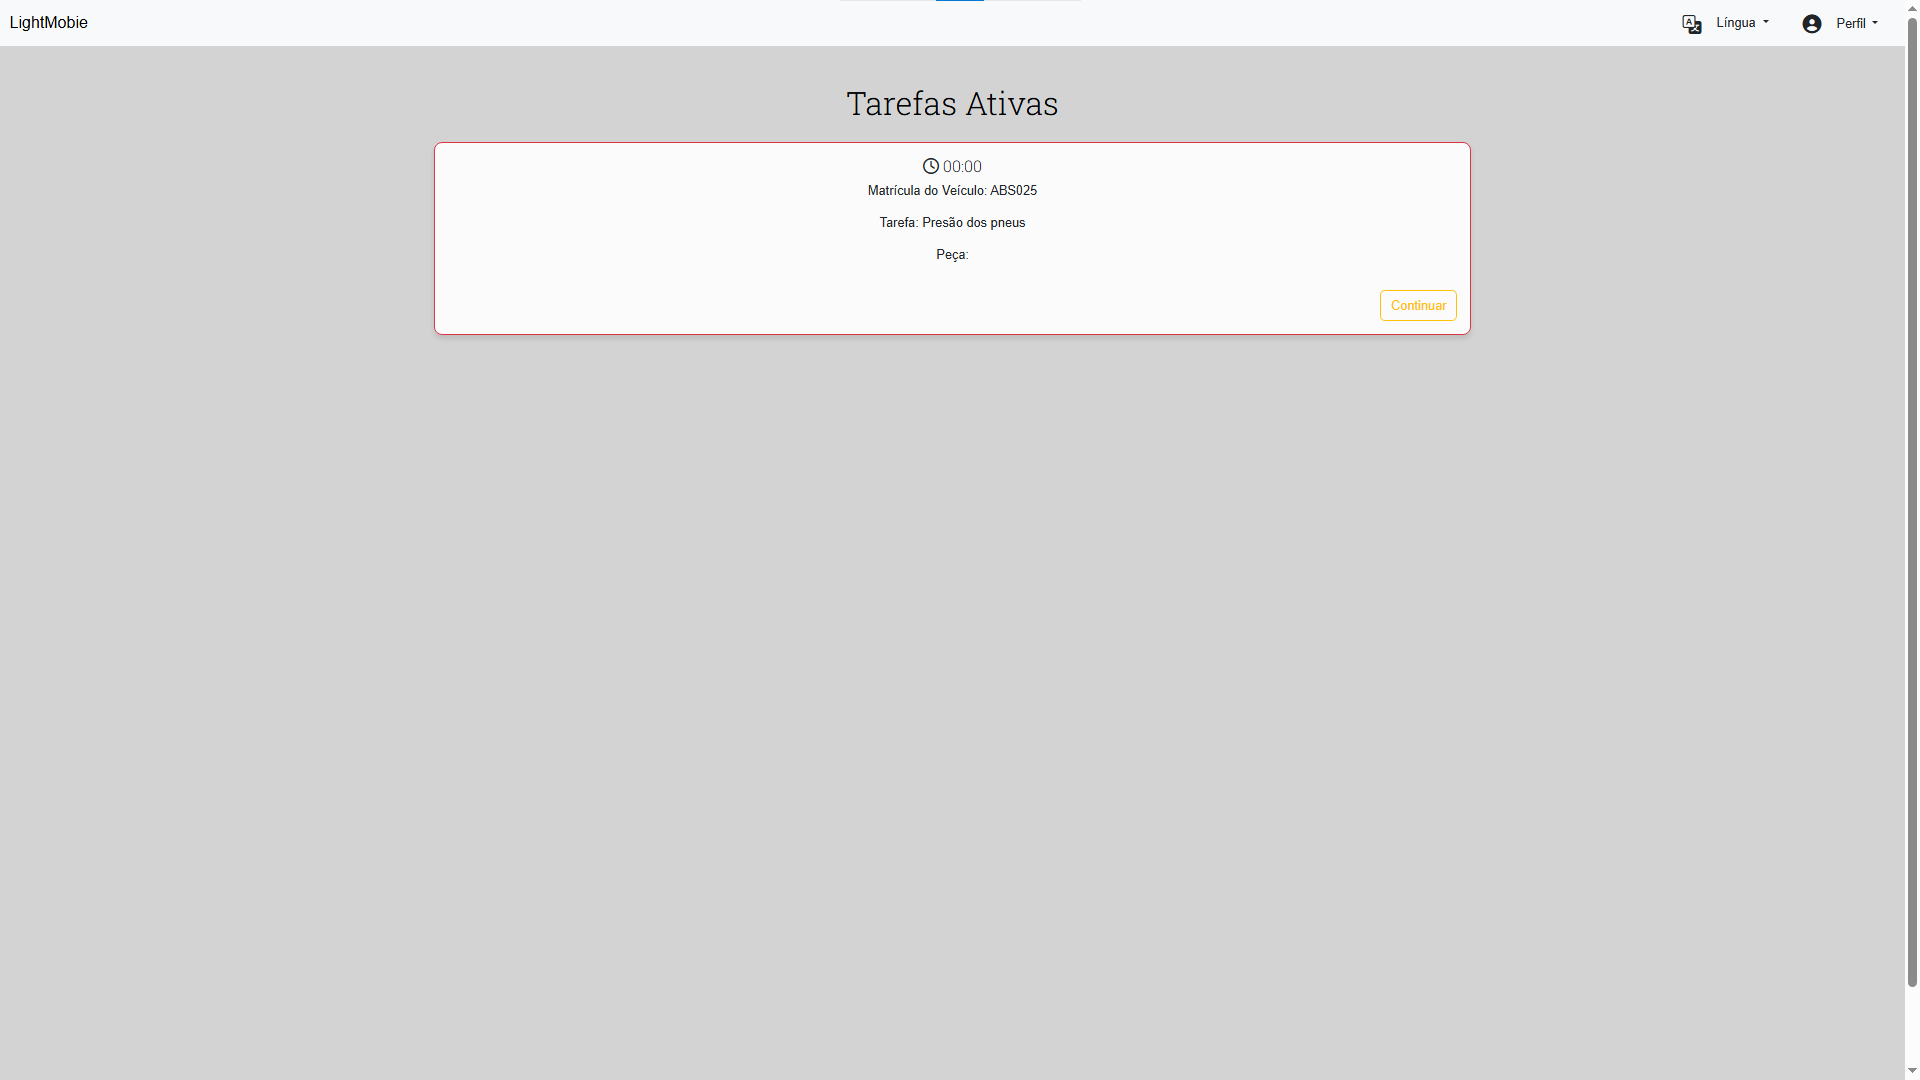
\includegraphics[width=\textwidth]{figs/Implementation/mechanic/HomeContinueLate}
  \label{fig:figure2}
\end{figure}



\begin{figure}[h]
  \caption{Mechanic home page with evaluation task.}
  \centering
  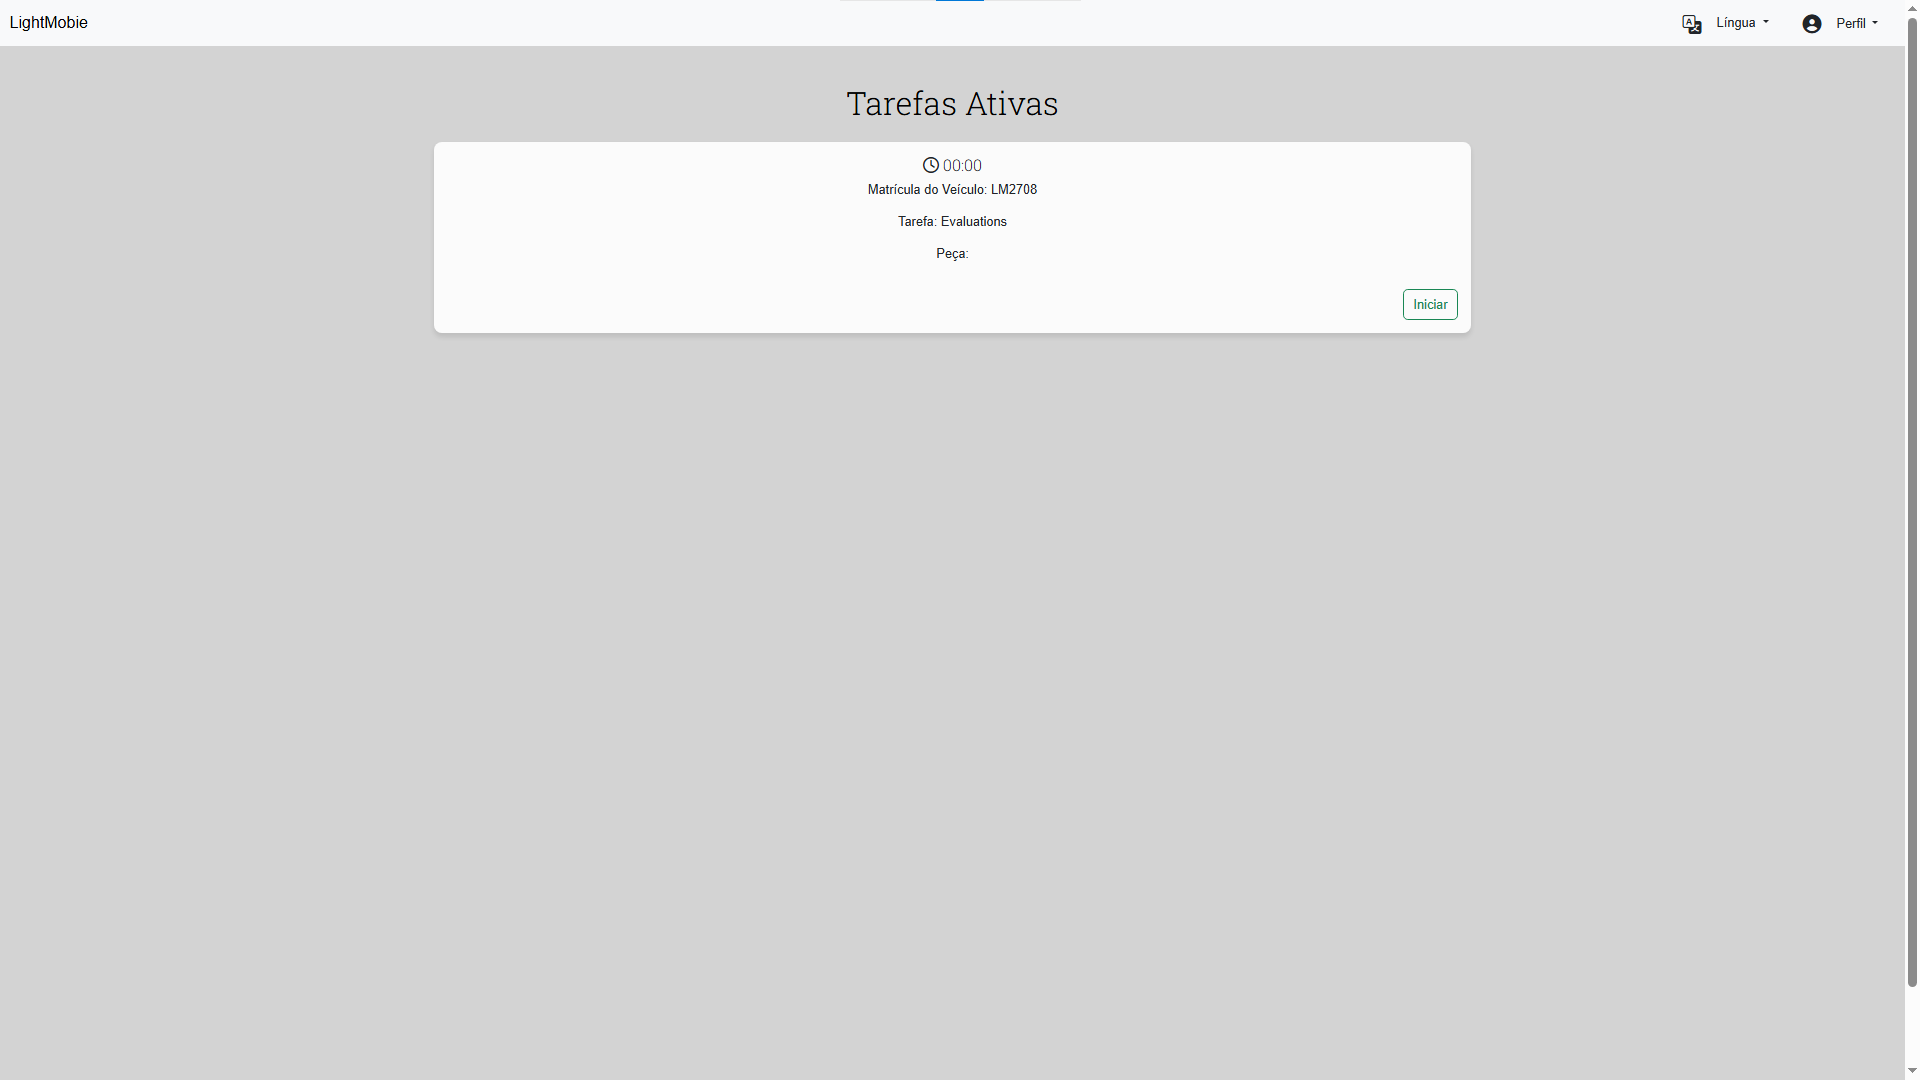
\includegraphics[width=\textwidth]{figs/Implementation/mechanic/HomeEvalNotLate}
  \label{fig:figure2}
\end{figure}

In this page the mechanic can see the tasks assigned to him for the day (Use Case 2.1 – View to-do list).
In the \ref we can see a task card with a red border and a yellow button with the value "Continue" (Use Case 2.6 – Continue Task).
This means the task was assigned to him to be done on a previous day and he already started the task but couldn't complete it so he paused it.

On the \ref we can see a evaluation task. A task has the following information:
- the vehicle registration
- the name of the task
- the part needed to completed the task, only appears if the task needs a part to be completed


\begin{figure}[h]
  \caption{Mechanic completing simple task first step.}
  \centering
  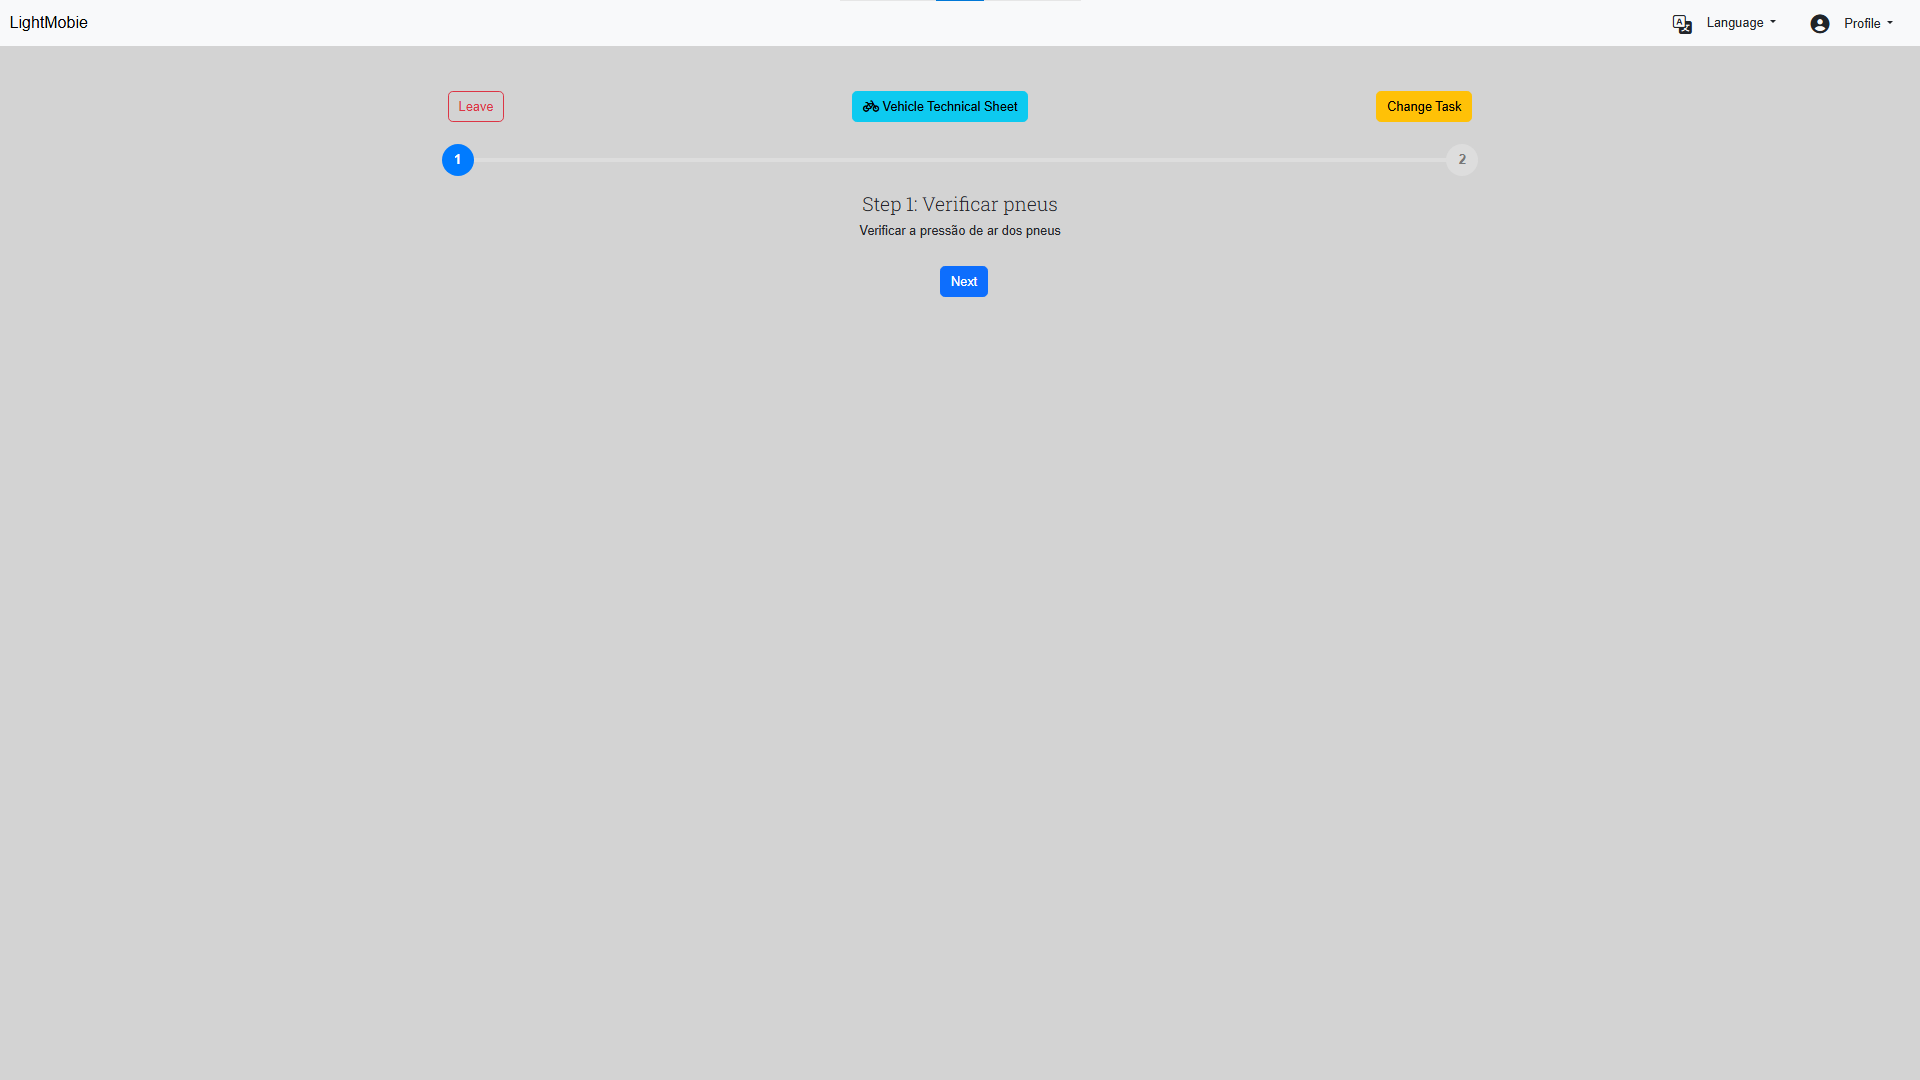
\includegraphics[width=\textwidth]{figs/Implementation/mechanic/MechanicTaskNormal}
  \label{fig:figure2}
\end{figure}

\begin{figure}[h]
  \caption{Vehicle details during a task completion.}
  \centering
  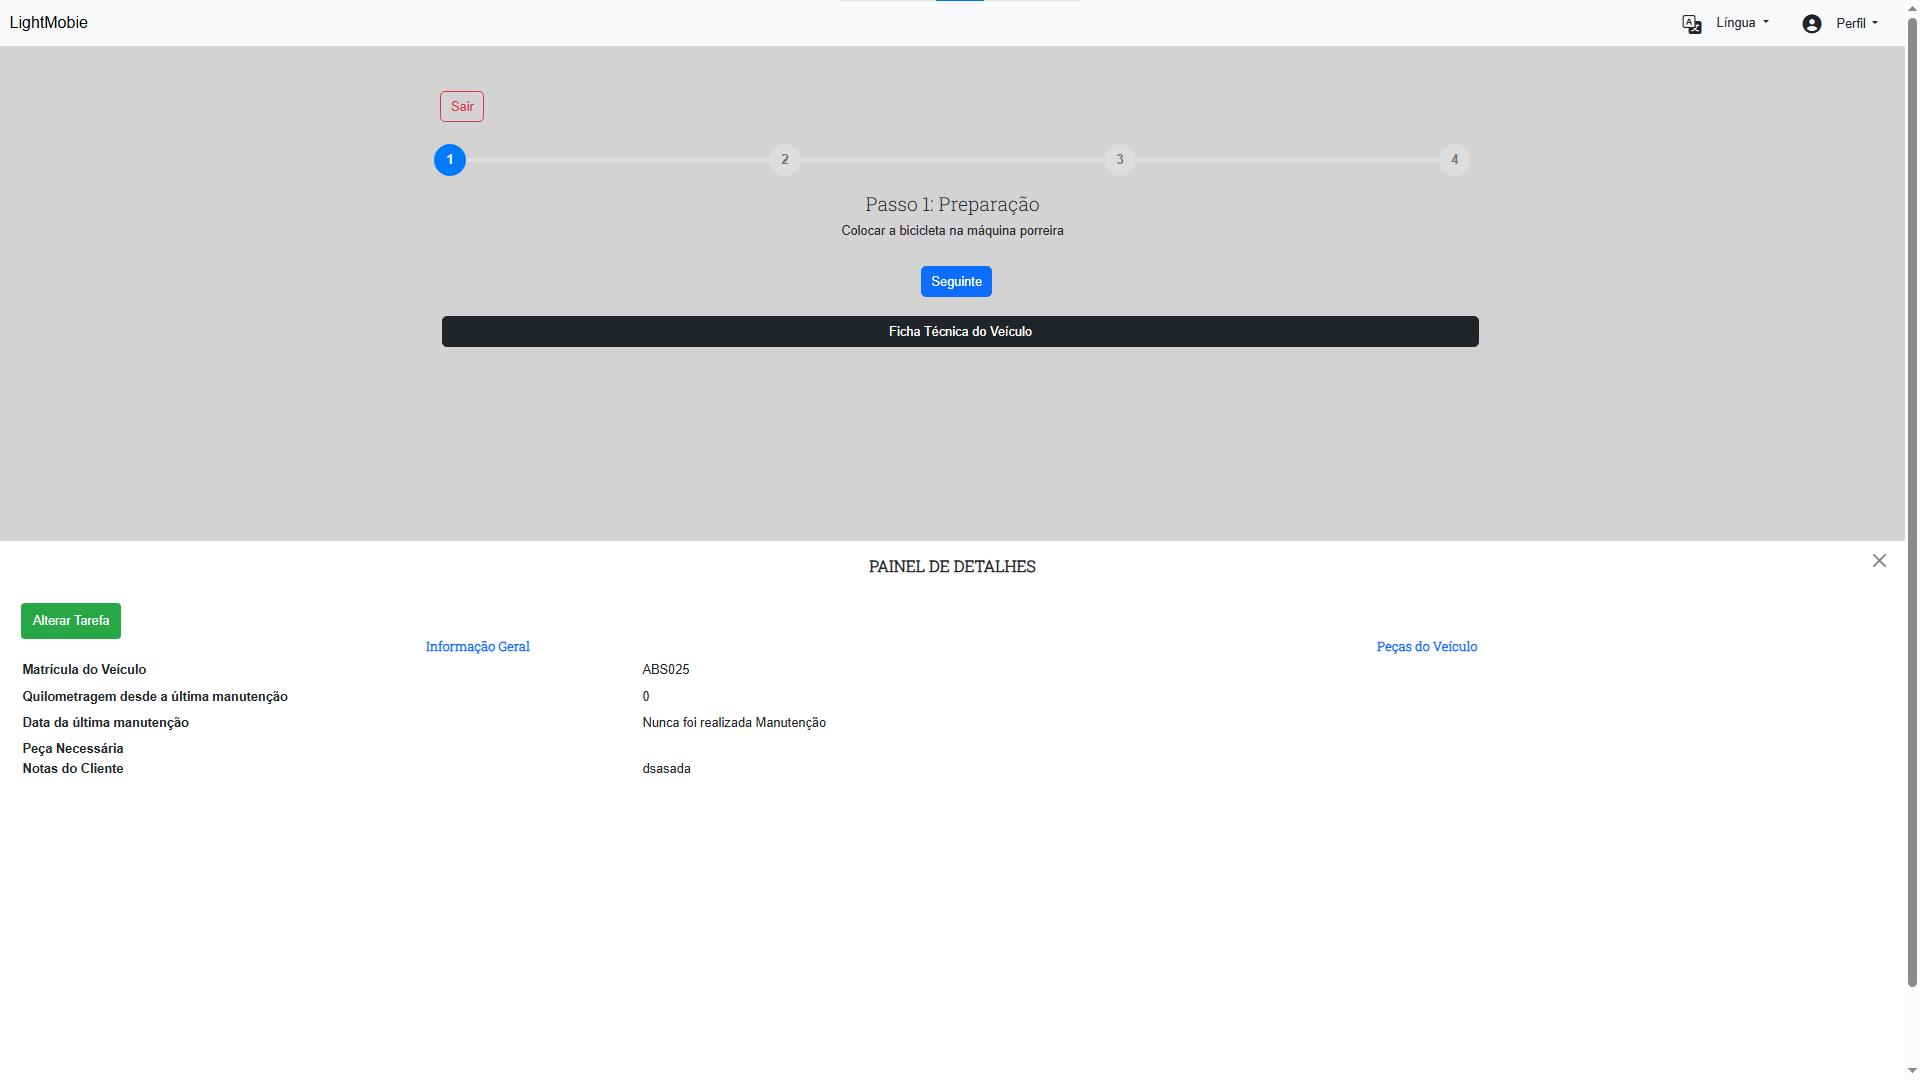
\includegraphics[width=\textwidth]{figs/Implementation/mechanic/MechanicTaskVehicleDetails}
  \label{fig:figure2}
\end{figure}

When clicking on the button "Continuar", it shows the steps to complete the task as seen in \ref.
In this page it has the name of the step, the description to complete the step, two buttons to navegate the through the step of the task, and a button to see the vehicle details.
When clicking on the button "Ficha tecnica do veículo" it shows a button offcanvas with the information of the vehicle as seen in \ref.
In this offcanvas is seen the following information:
- vehicle Registration
- Number of Kilometers since the last maintenance
- date of the last maintenance
- necessary part to complete the task
- the client notes
- the name of the parts of the vehicle and the date they were added to it


\begin{figure}[h]
  \caption{Change task modal.}
  \centering
  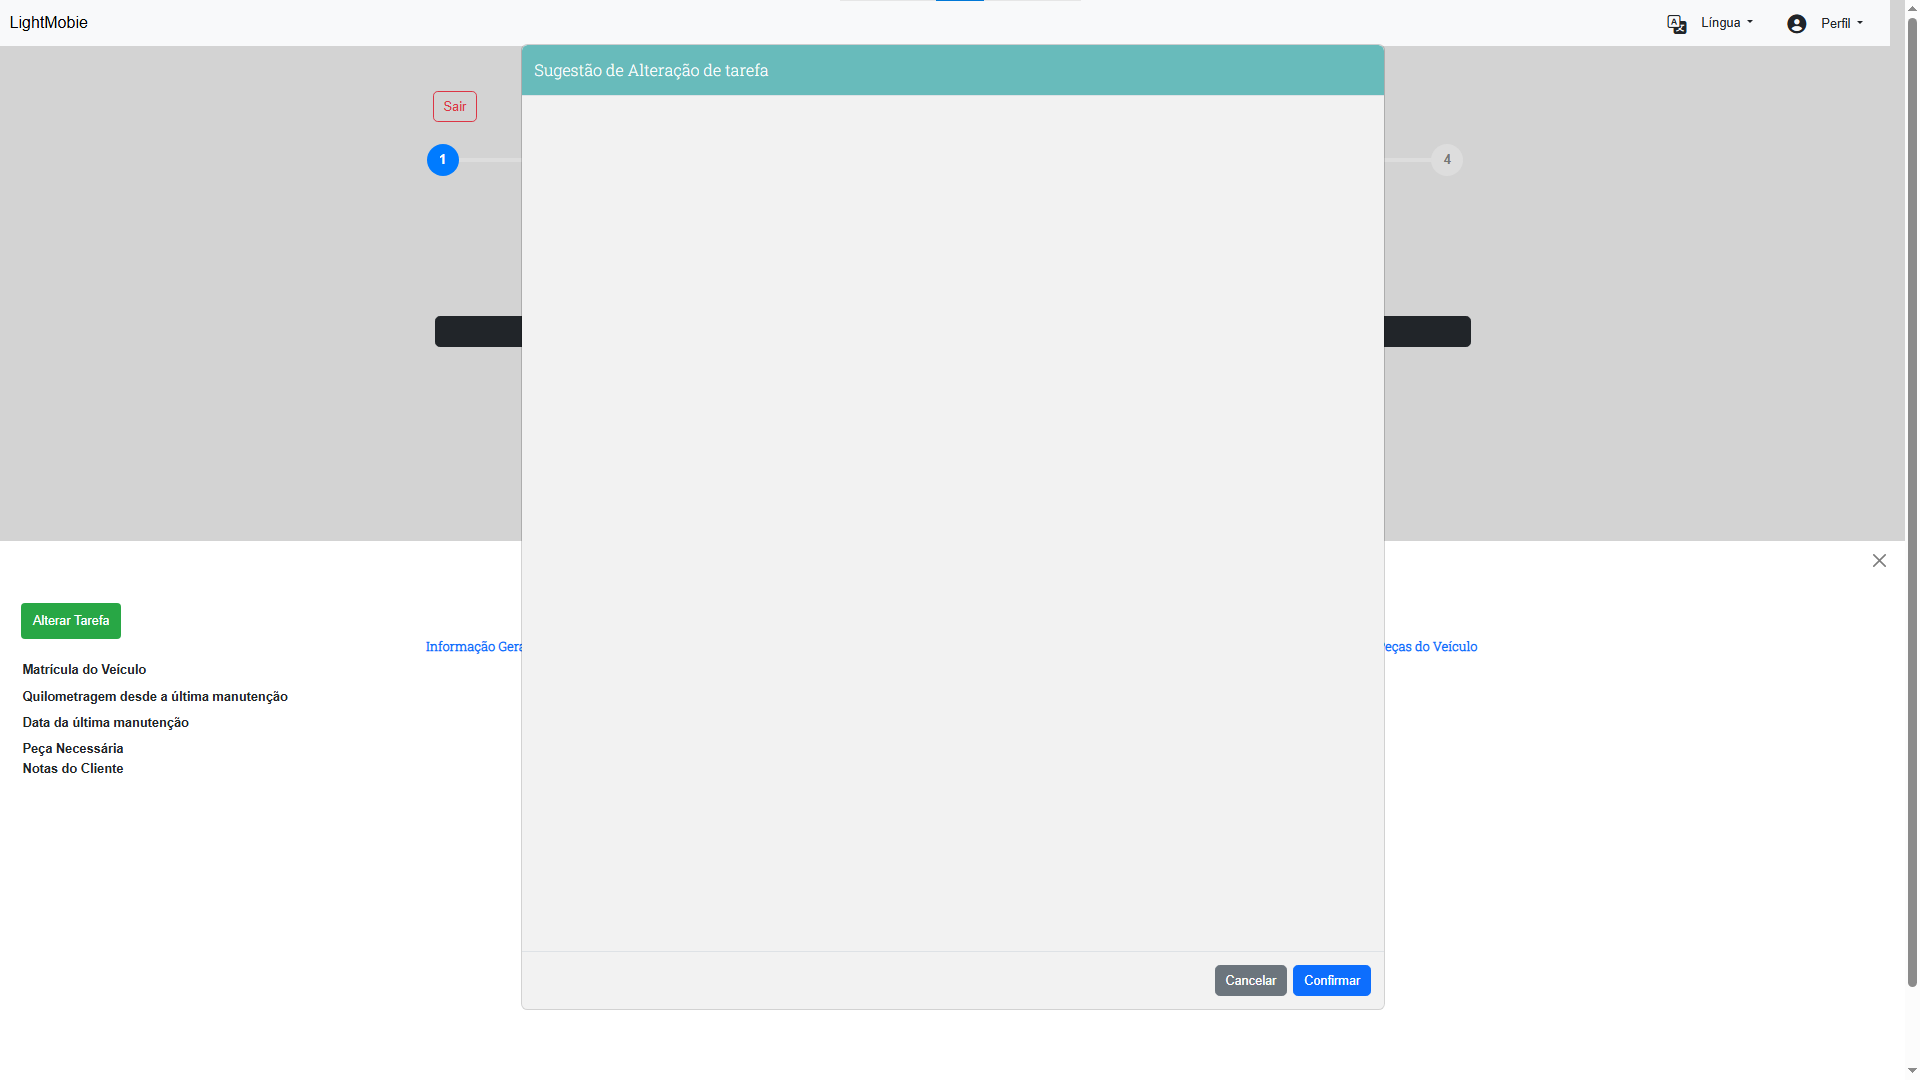
\includegraphics[width=\textwidth]{figs/Implementation/mechanic/MechanicTaskChangeTask}
  \label{fig:figure2}
\end{figure}

In this offcanvas there is also a button "Alterar Tarefa" to change the part of the task.
When clicking in this button it shows a modal with a select with the part the mechanic wants to replace, and by eating the button "Confirmar" the tasks is paused and a maintenance change is generated.
with this the Use Case 2.5 – Change Task is completed.


\begin{figure}[h]
  \caption{Mechanic task last step.}
  \centering
  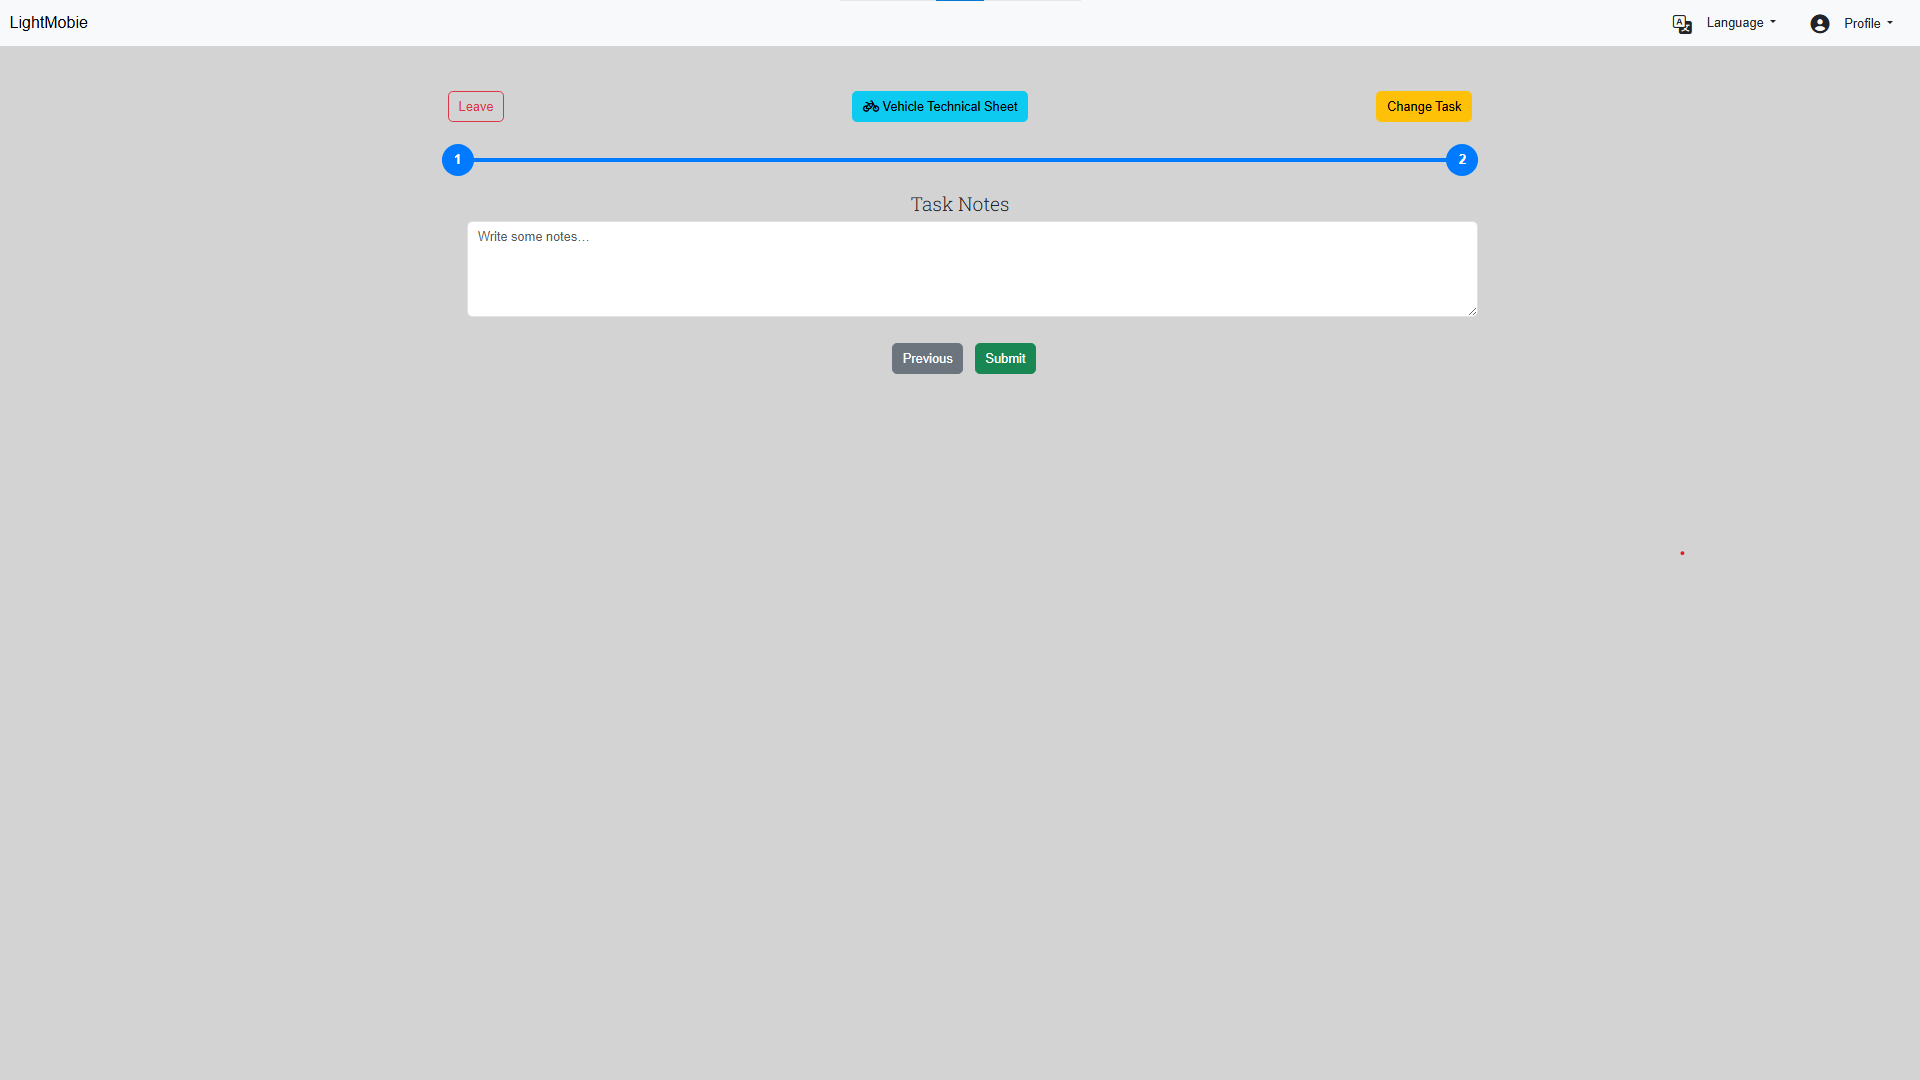
\includegraphics[width=\textwidth]{figs/Implementation/mechanic/MechanicTaskLastStep}
  \label{fig:figure2}
\end{figure}

By following the steps of the task the mechanic will reach the last step where he can leave some notes and complete the task, accomplish the Use Case 2.4 – Do a Vehicle maintenance task. As seen in \ref.


\begin{figure}[h]
  \caption{Mechanic Evaluation first step.}
  \centering
  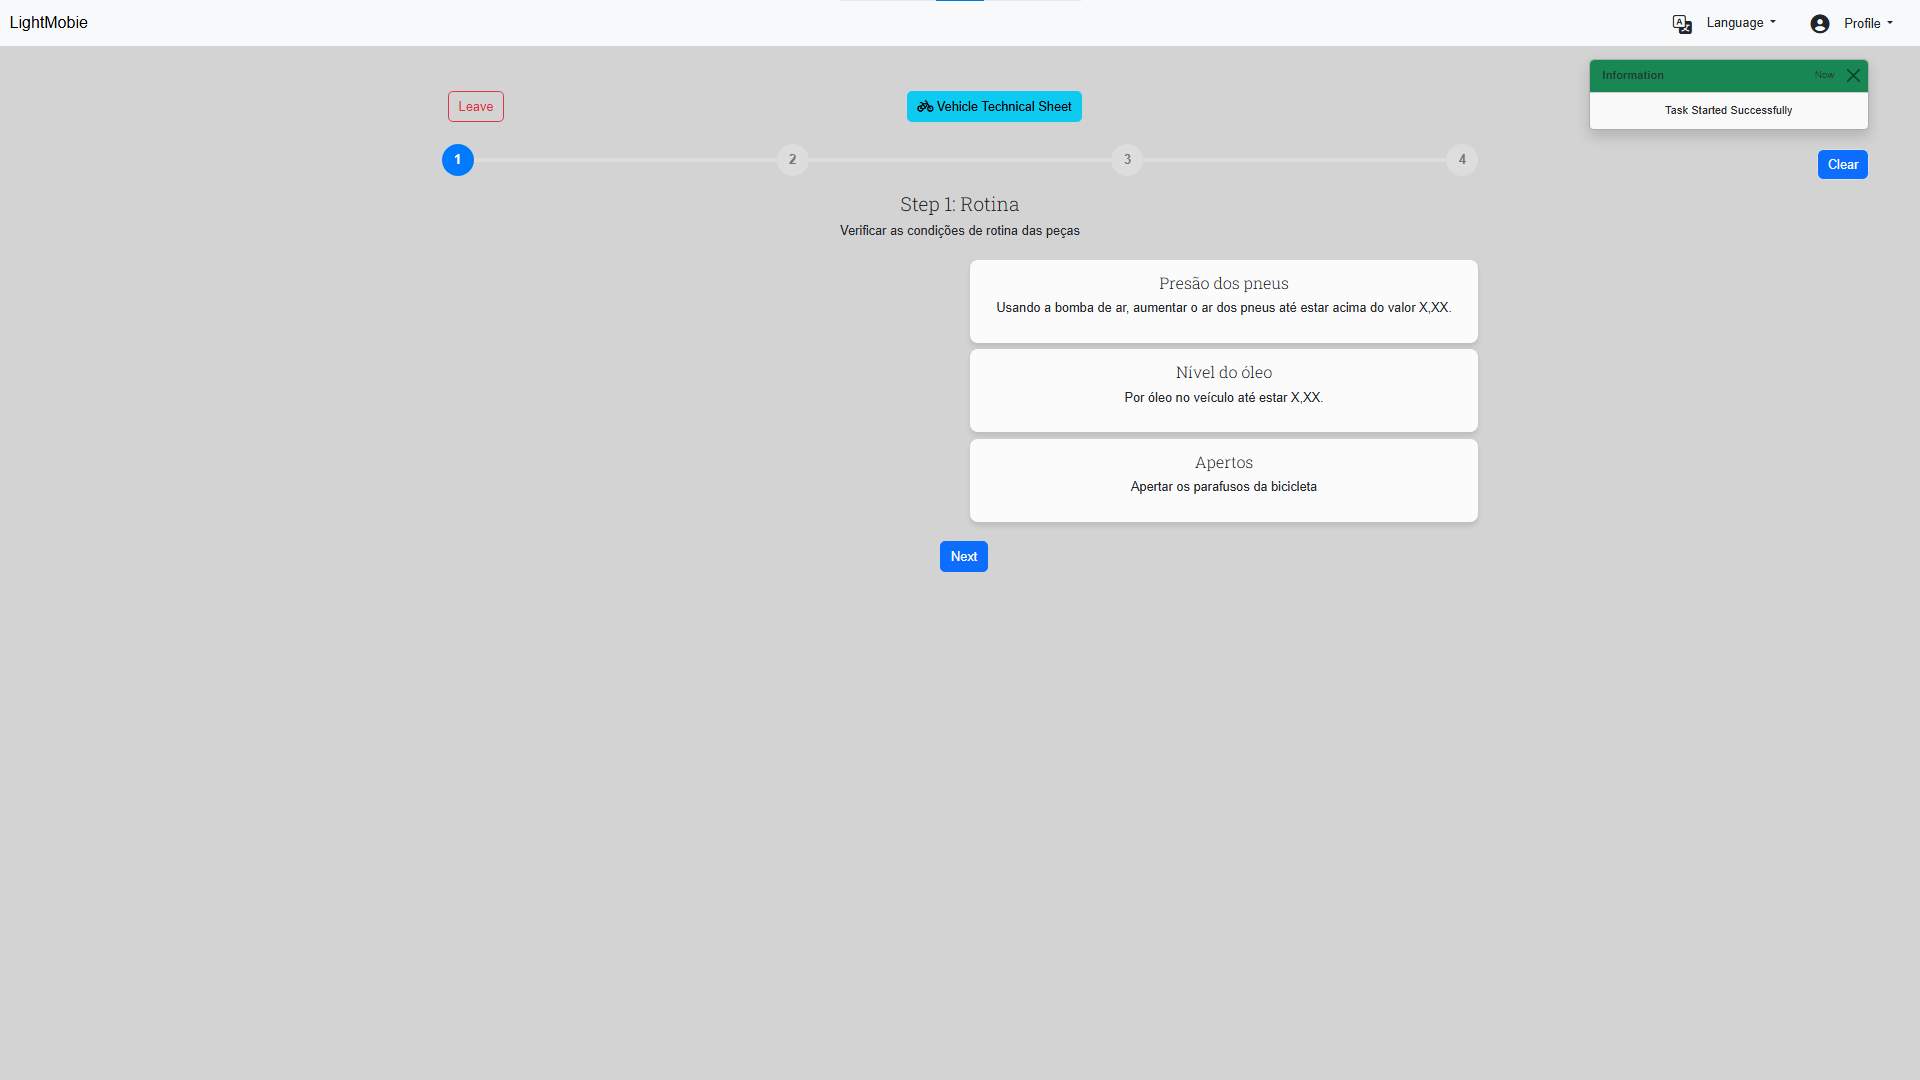
\includegraphics[width=\textwidth]{figs/Implementation/mechanic/MechanicEvaluationNormal}
  \label{fig:figure2}
\end{figure}



\begin{figure}[h]
  \caption{Mechanic select part modal.}
  \centering
  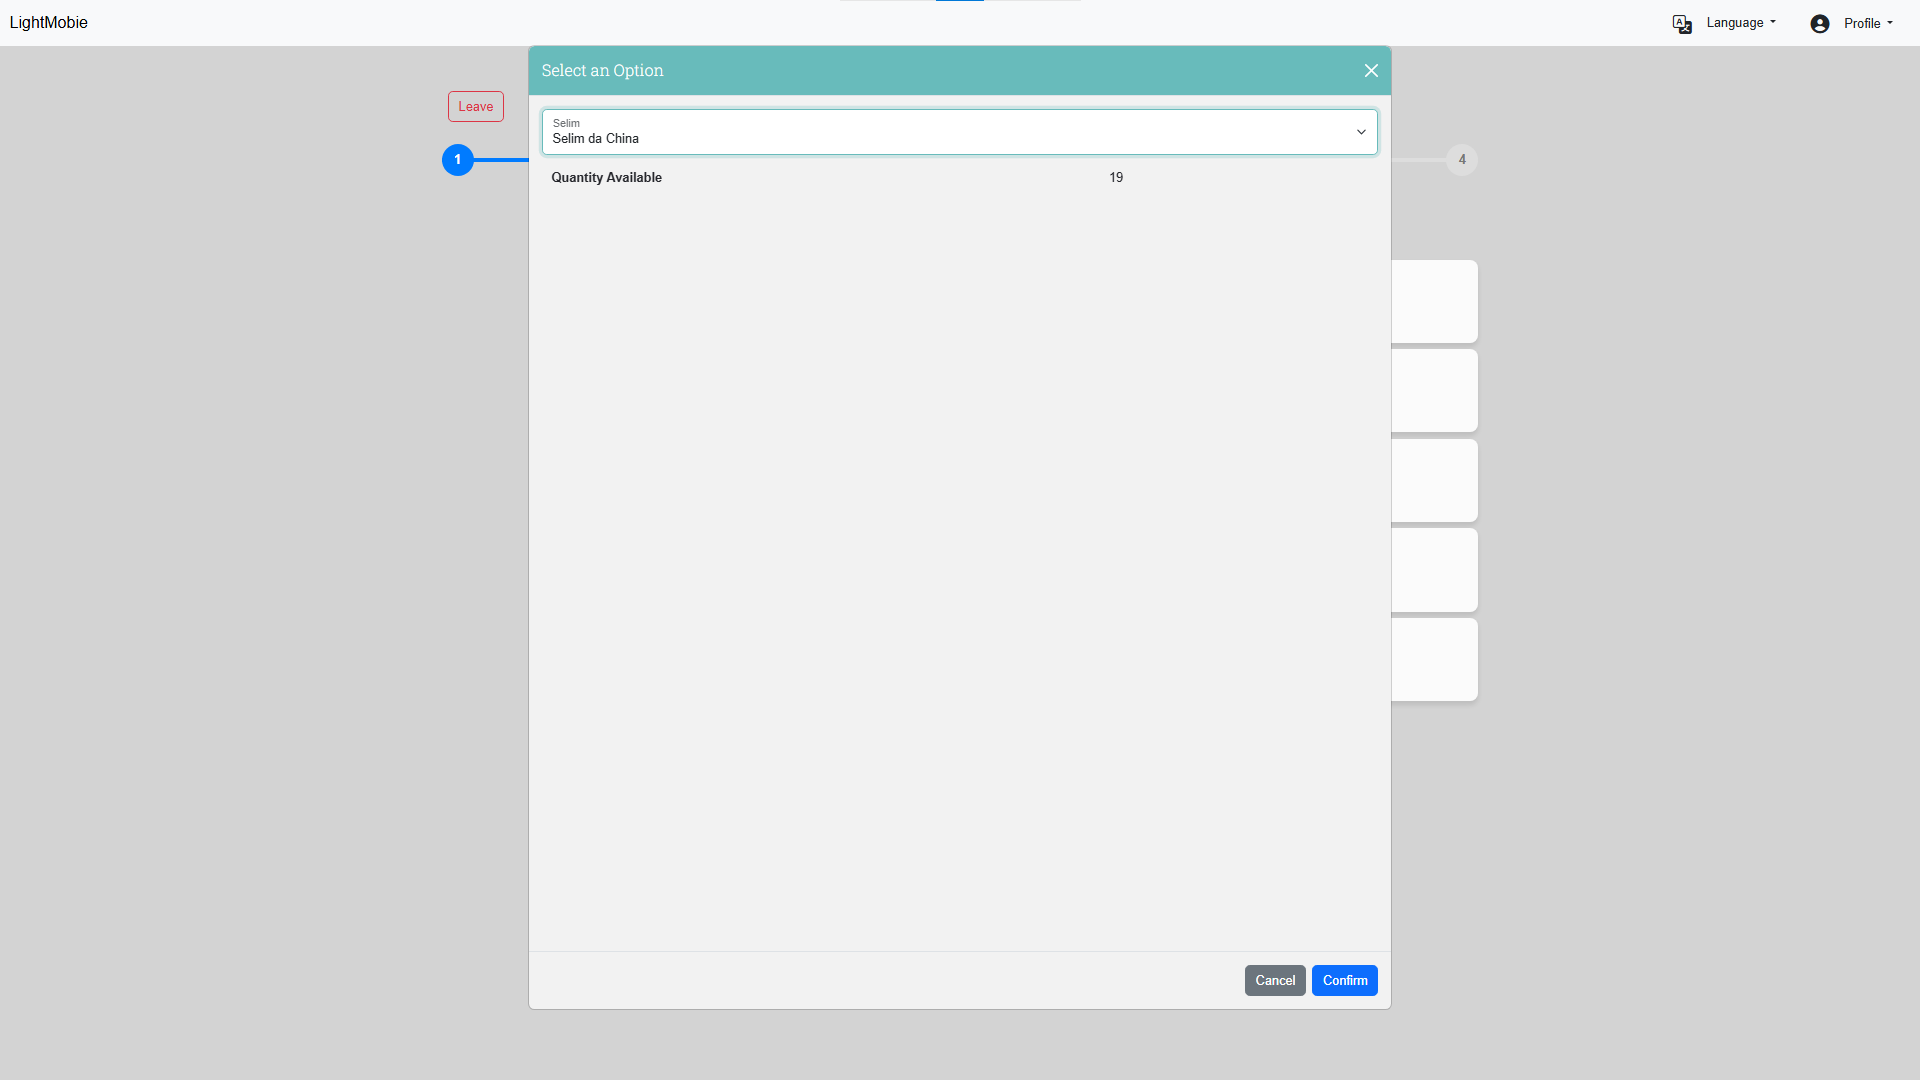
\includegraphics[width=\textwidth]{figs/Implementation/mechanic/MechanicEvaluationSelectTaskWitPart}
  \label{fig:figure2}
\end{figure}

\begin{figure}[h]
  \caption{Mechanic Evaluation task with part selected.}
  \centering
  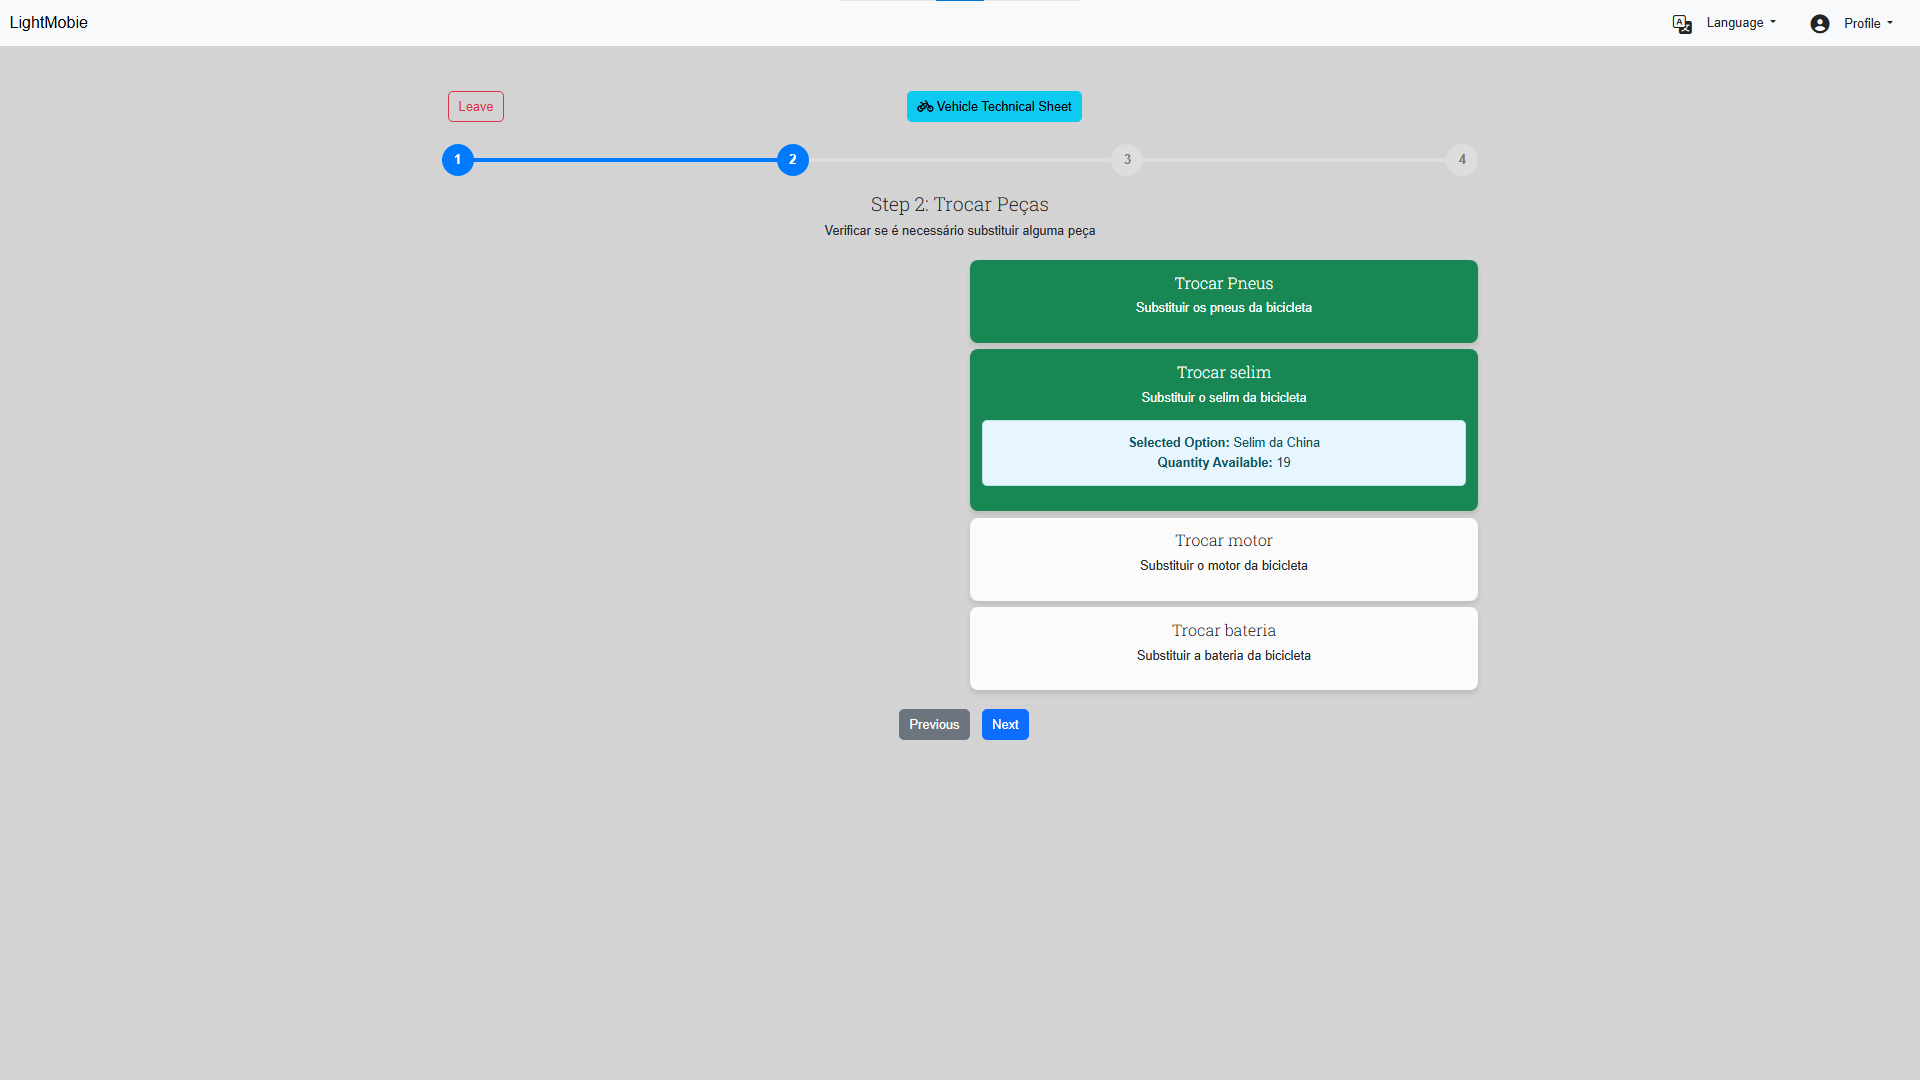
\includegraphics[width=\textwidth]{figs/Implementation/mechanic/TaskSelected}
  \label{fig:figure2}
\end{figure}

when clicking on the "Começar" button on the figure \ref, it appear a toast notification informing the mechanic started the task and a list of tasks the mechanic can add to the maintenance, seen in \ref.
This page has also the button "Ficha tecnica do vehicle" with the same information as the simple task.
When a task is selected it turns green, but if the tasks needs a part to be completed it first opens a modal where the mechanic needs to select the part need to complete the task, as seen in figure \ref.
It shows the number of parts available in the warehouse to inform the mechanic if he would like to change the task since there are few or no parts.
After that, the part turns green as seen in the figure \ref.

\begin{figure}[h]
  \caption{Mechanic Evaluation last step.}
  \centering
  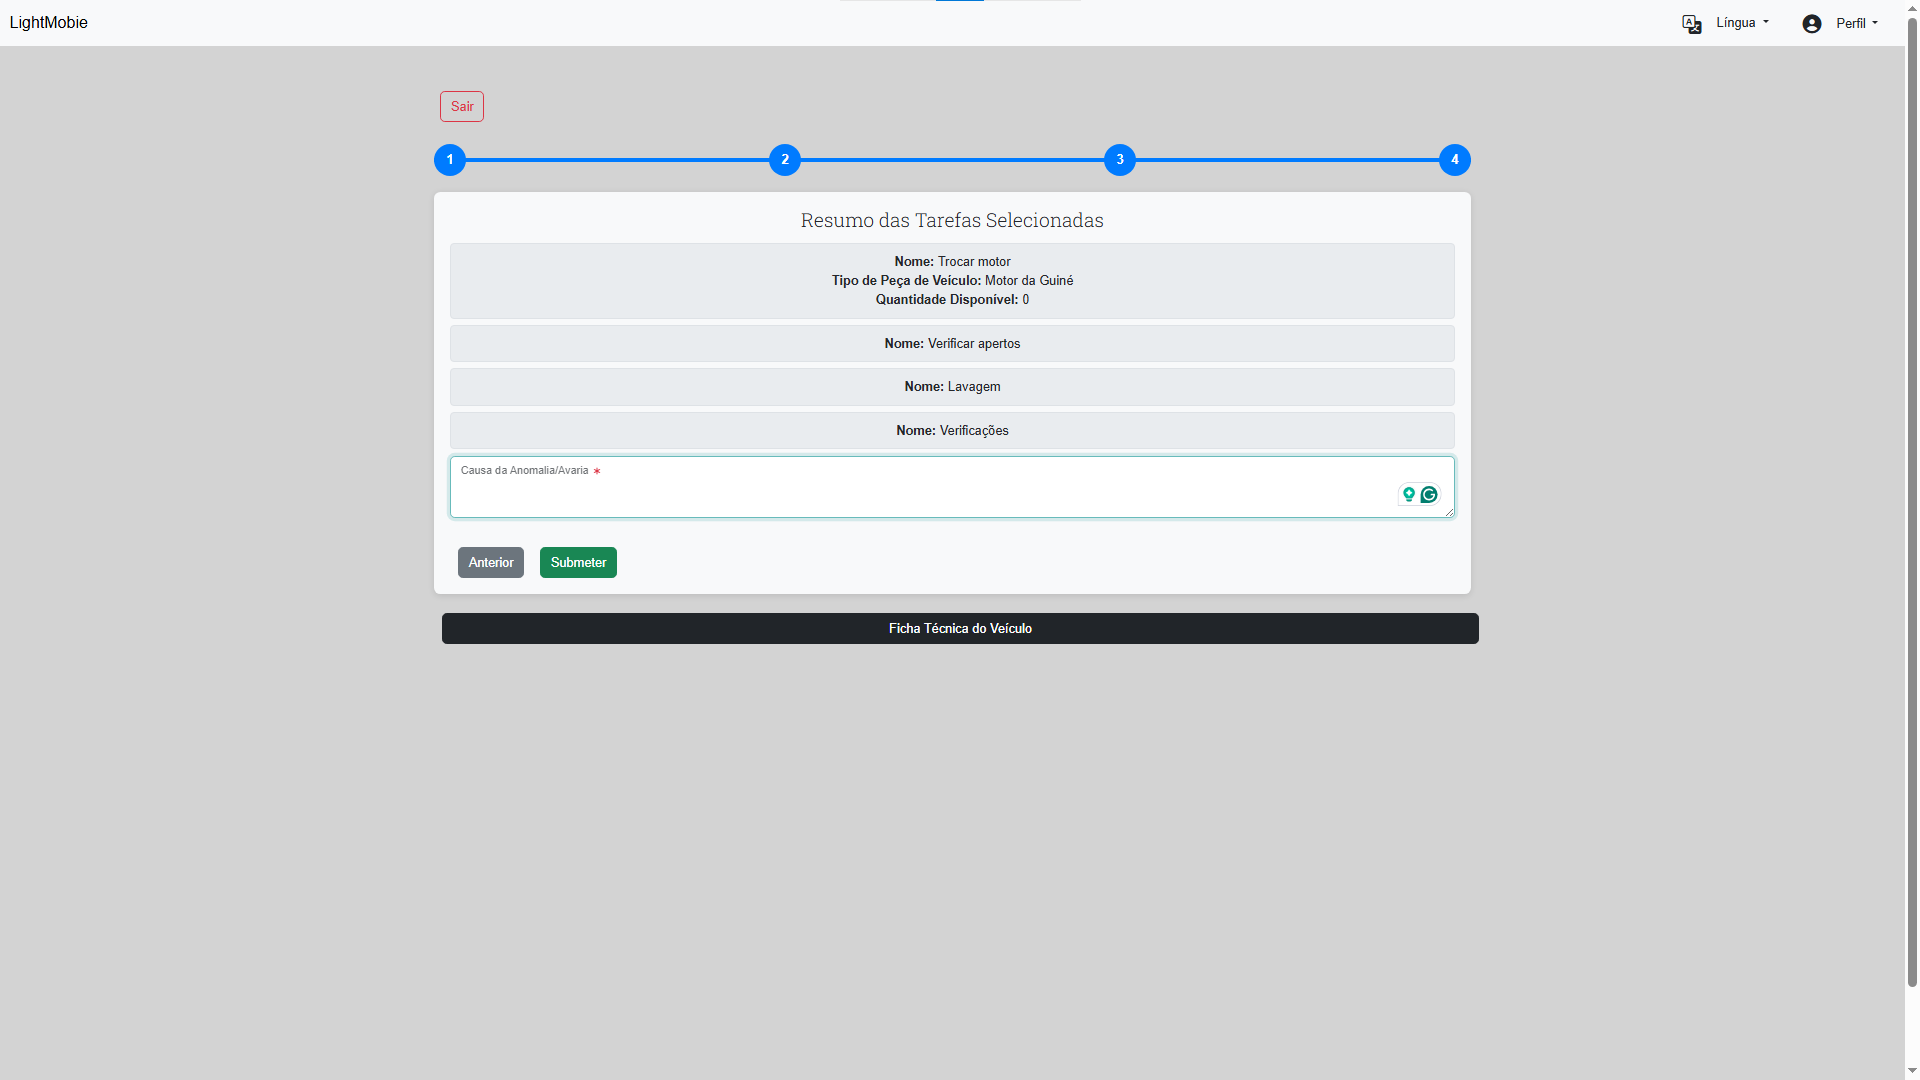
\includegraphics[width=\textwidth]{figs/Implementation/mechanic/EvaluationLastStep}
  \label{fig:figure2}
\end{figure}

As the mechanic follows the steps he goes to the last step where he sees the selected tasks and he needs to describe the cause of the anomaly before finishing the task.
when finishing the task, mechanic is notified by toast notification that the task is completed and with this the Use Case 2.2 – Carry out a vehicle analysis or the Use Case 2.3 – Register tasks completed are completed depending if its a dealership performing a maintenance on the vehicle of the bike sharing entity with efficiency aim maintenance.



\subsection{Warehouse Operator view}

\begin{figure}[h]
  \caption{Warehouse home page.}
  \centering
  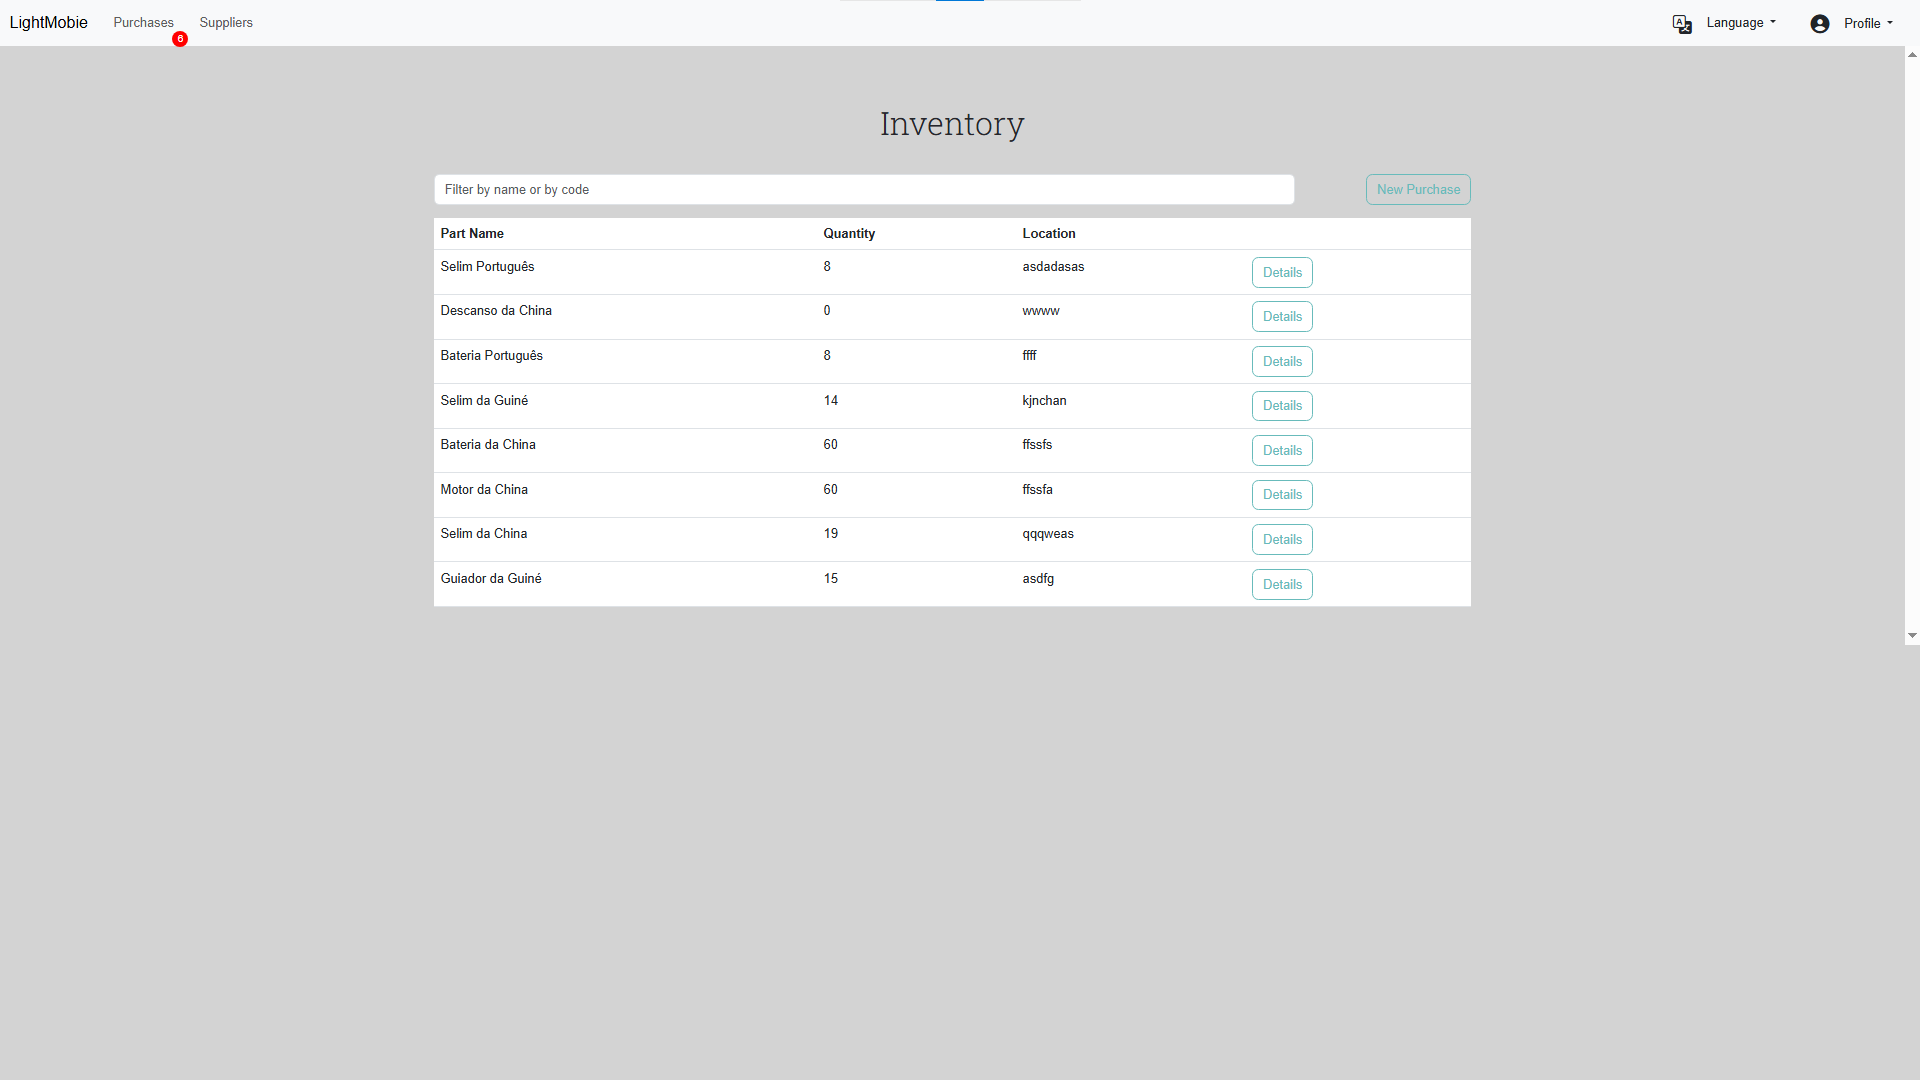
\includegraphics[width=\textwidth]{figs/Implementation/warehouse/homepage}
  \label{fig:figure2}
\end{figure}
The warehouse operator view layout strcuture is very similar as the other views as seen in \ref.
It has the menu on the top of the page and where we can see the list of purchases and the list of suppliers, and has the inventory in the body of the page (Use Case 3.1 – View the different parts that the warehouse possess).
This inventory is composed of a table of parts in the warehouse including the number of parts available and the location code to locate it.
If we want to know more about a part we can click on the respective "Detalhes" button and will open a modal, as seen in \ref.

\begin{figure}[h]
  \caption{Inventory details.}
  \centering
  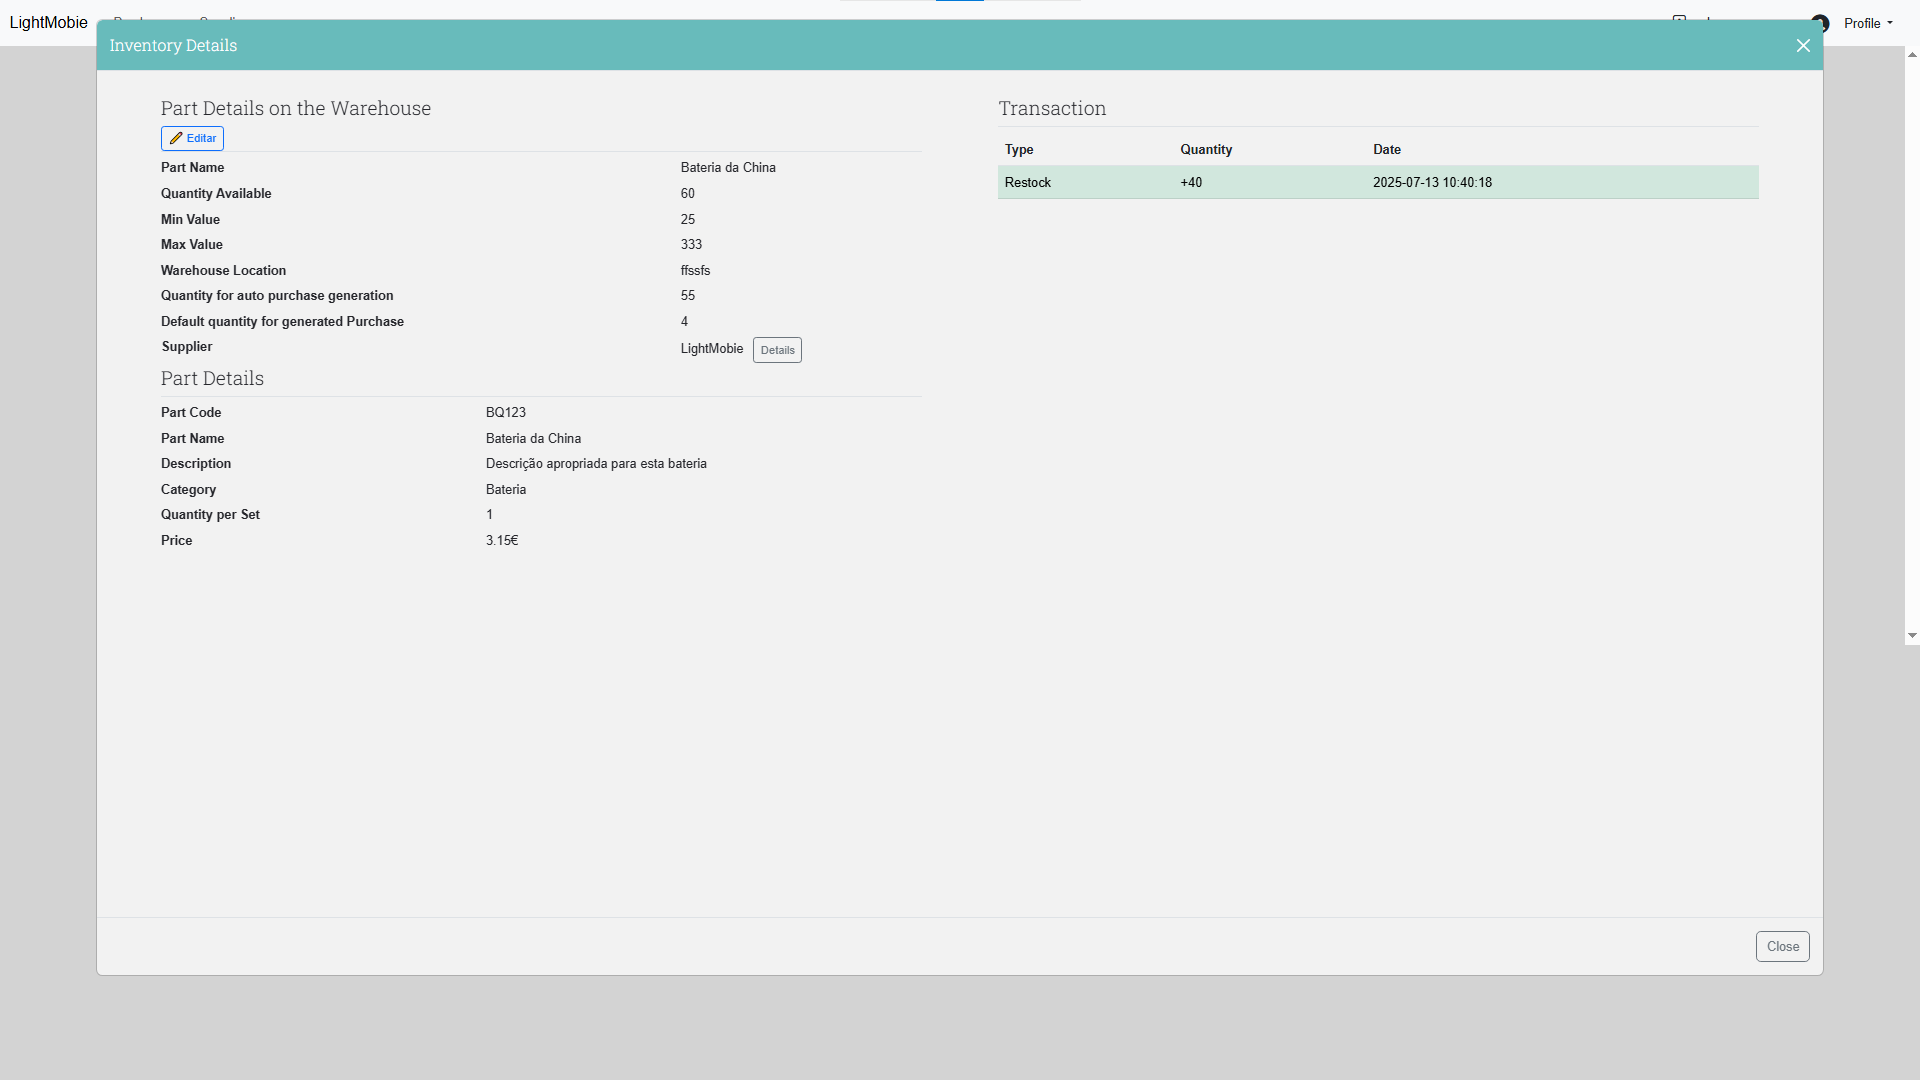
\includegraphics[width=\textwidth]{figs/Implementation/warehouse/inventoryDetails}
  \label{fig:figure2}
\end{figure}

In the modal, we can see the transaction history of the parts; which means the quantity and the date when thes parts were added or removed from the inventory.
We can also see other information about the part:
- The name of the part
- the quantity available
- the minimum quantity
- the maximum quantity
- the location on the warehouse
- the default quantity to generate a purchase
- the quantity to use when occurr an automatic purchase generation
- the code of the part
- the description of the part
- the category of the part
- the quantity per group
- the price of the part


\begin{figure}[h]
  \caption{Inventory editor.}
  \centering
  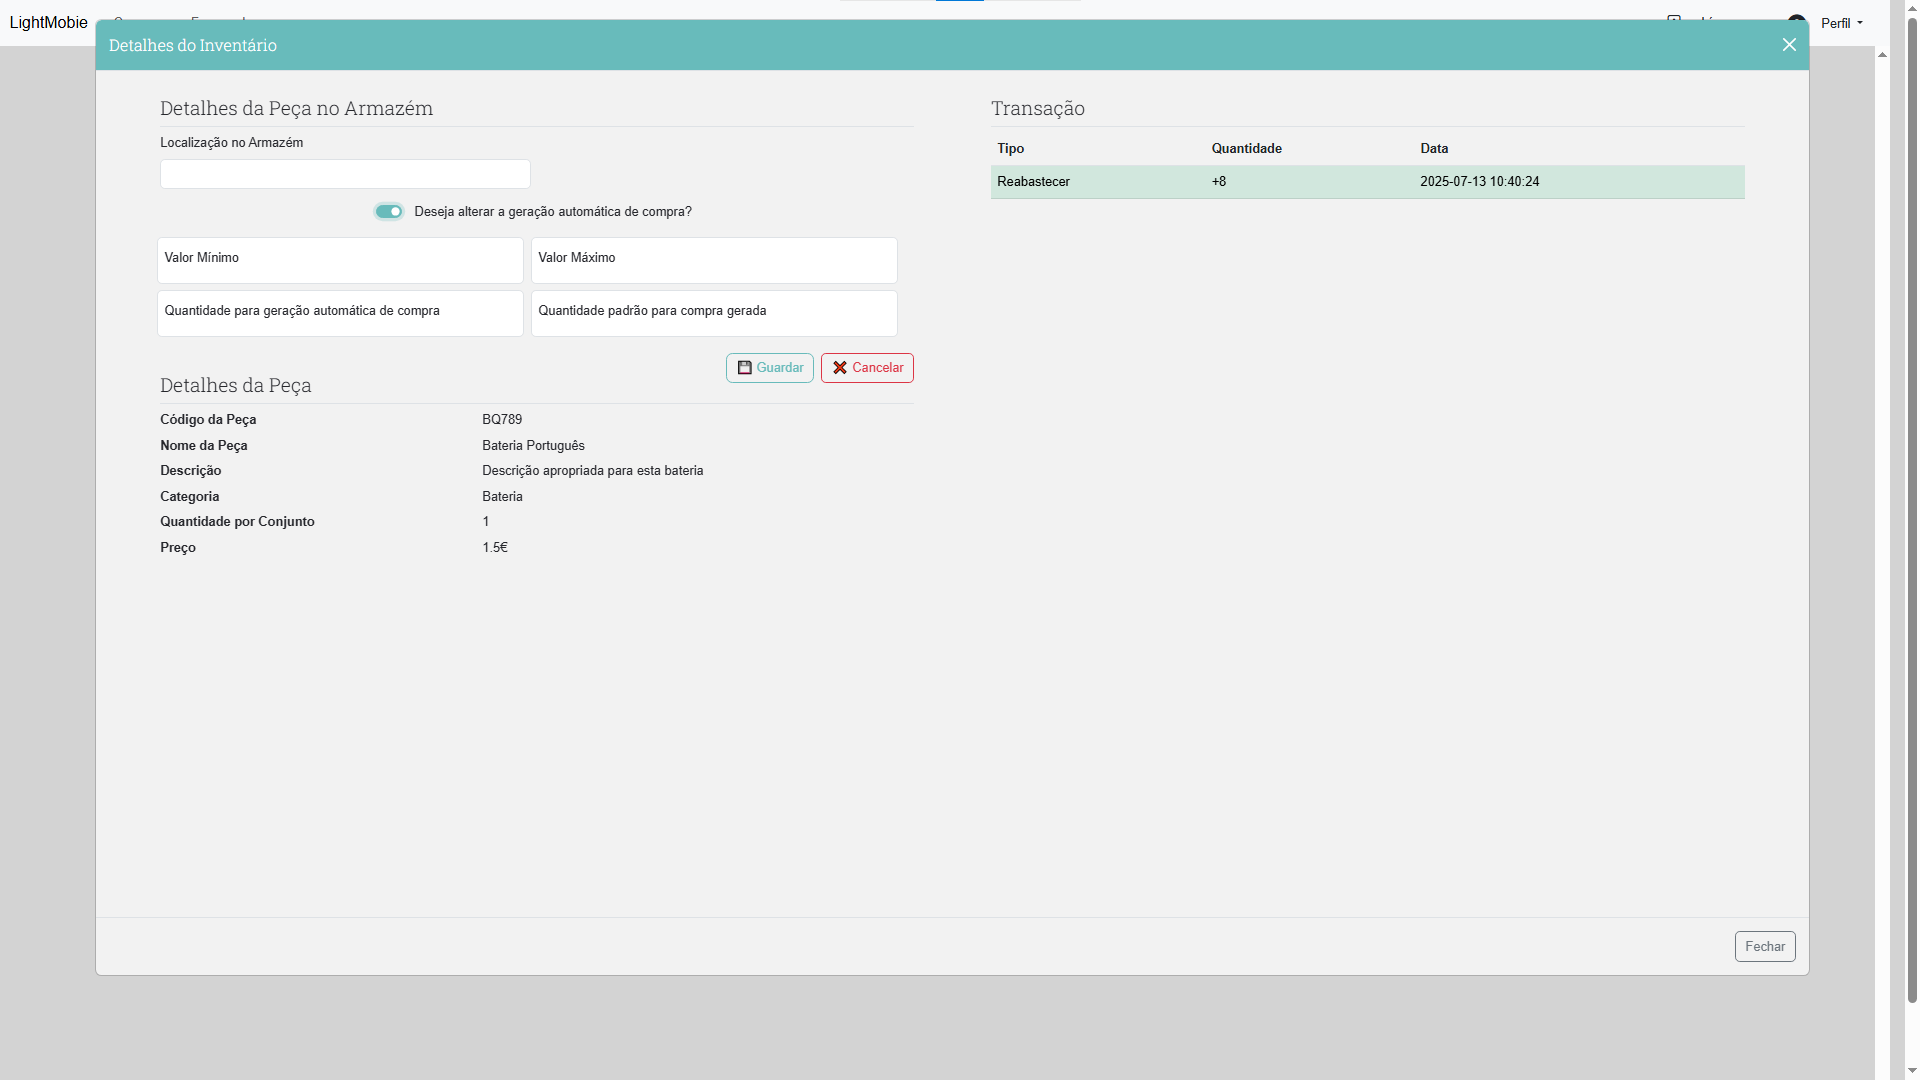
\includegraphics[width=\textwidth]{figs/Implementation/warehouse/inventoryEdit}
  \label{fig:figure2}
\end{figure}

It is possible to edit the inventory clicking on the button "Editar" (Use Case 3.5 – Edit Inventory ) and will show a form as seen in \ref.
In here we can change:
- the location of the part in the warehouse
- the minimum quantity of the part
- the maximum quantity of the part
- the quantity to generate a maximum purchase
- the quantity use on the automatic generated purchase

\begin{figure}[h]
  \caption{Create new purchase modal.}
  \centering
  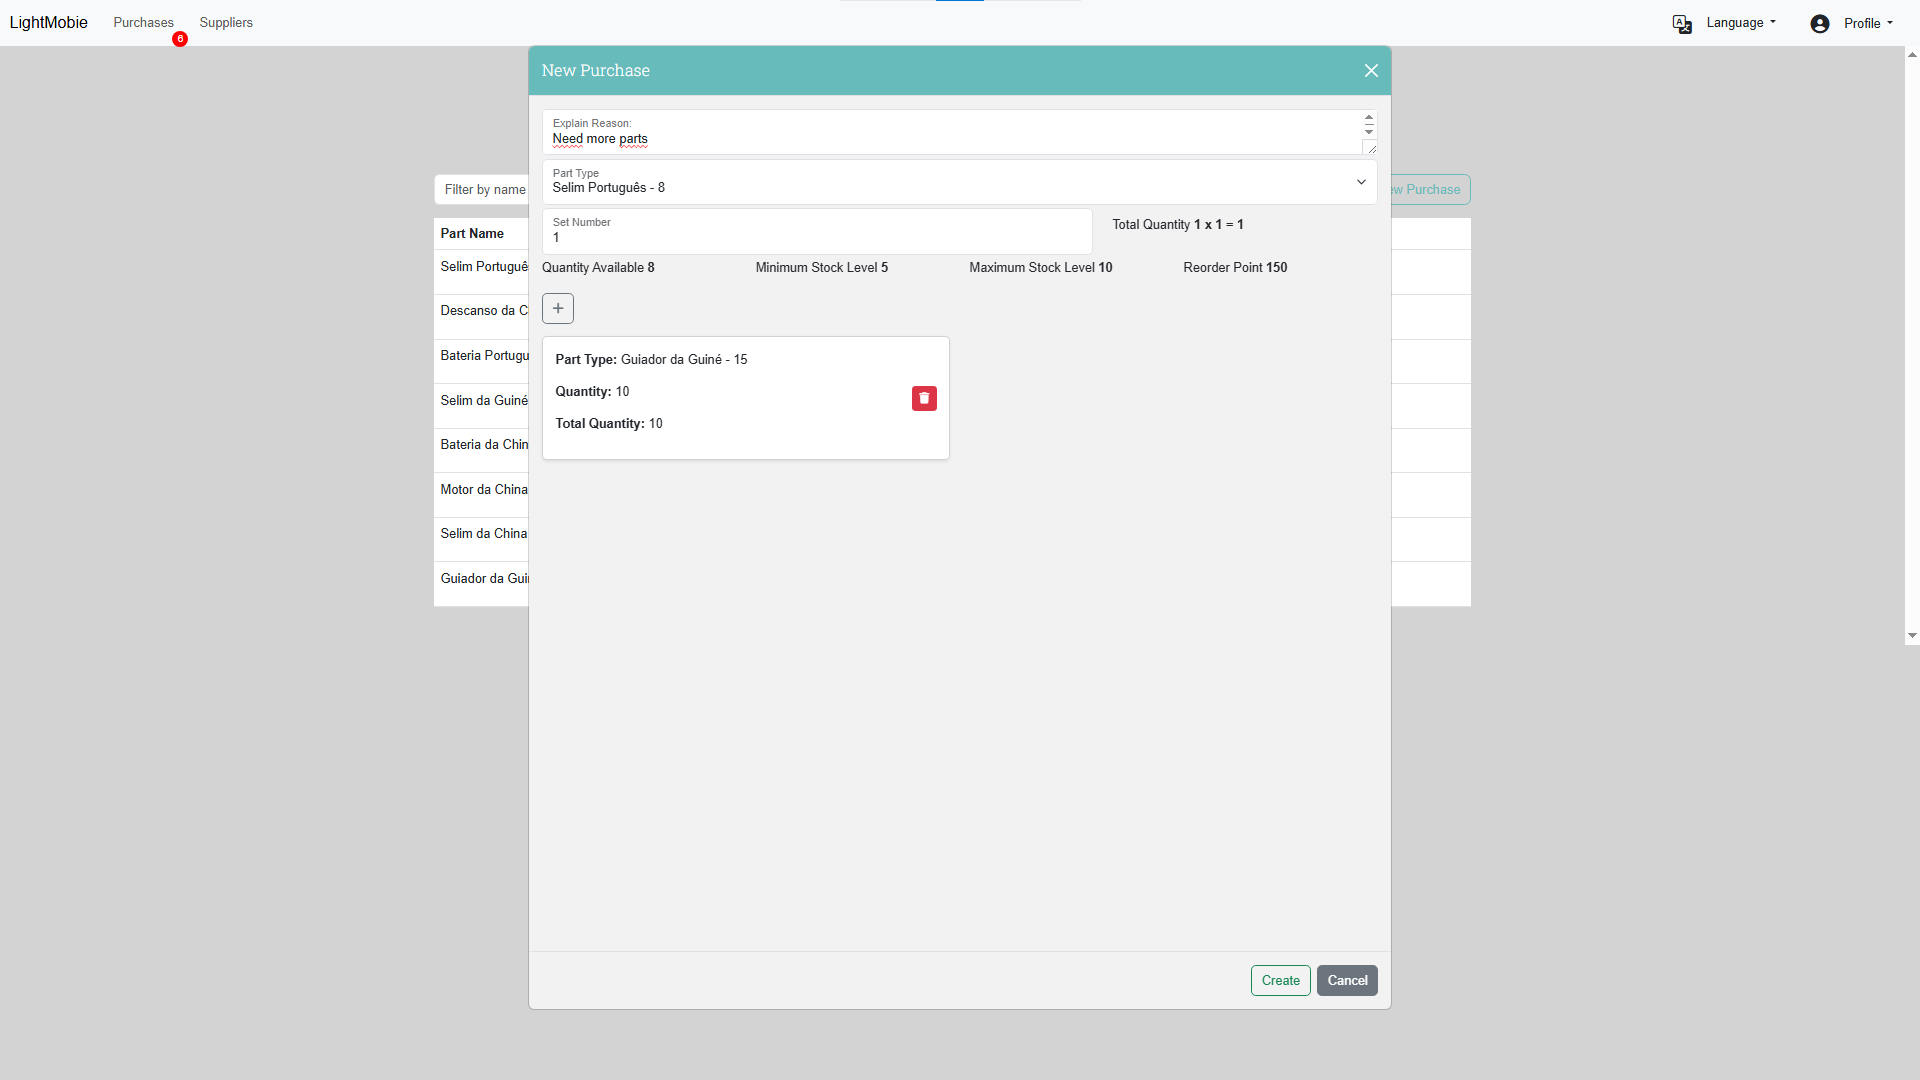
\includegraphics[width=\textwidth]{figs/Implementation/warehouse/createPurchase}
  \label{fig:figure2}
\end{figure}

Returning to the homepage, we can see a search bar on the top of the table that can be use to filter the parts by name, and a button to create a new purchase on the right side of it (Use Case 3.2 – Requesting purchasing service).
By clicking in this button will show a modal as seen in \ref.

\begin{figure}[h]
  \caption{Create new purchase modal with a part selected.}
  \centering
  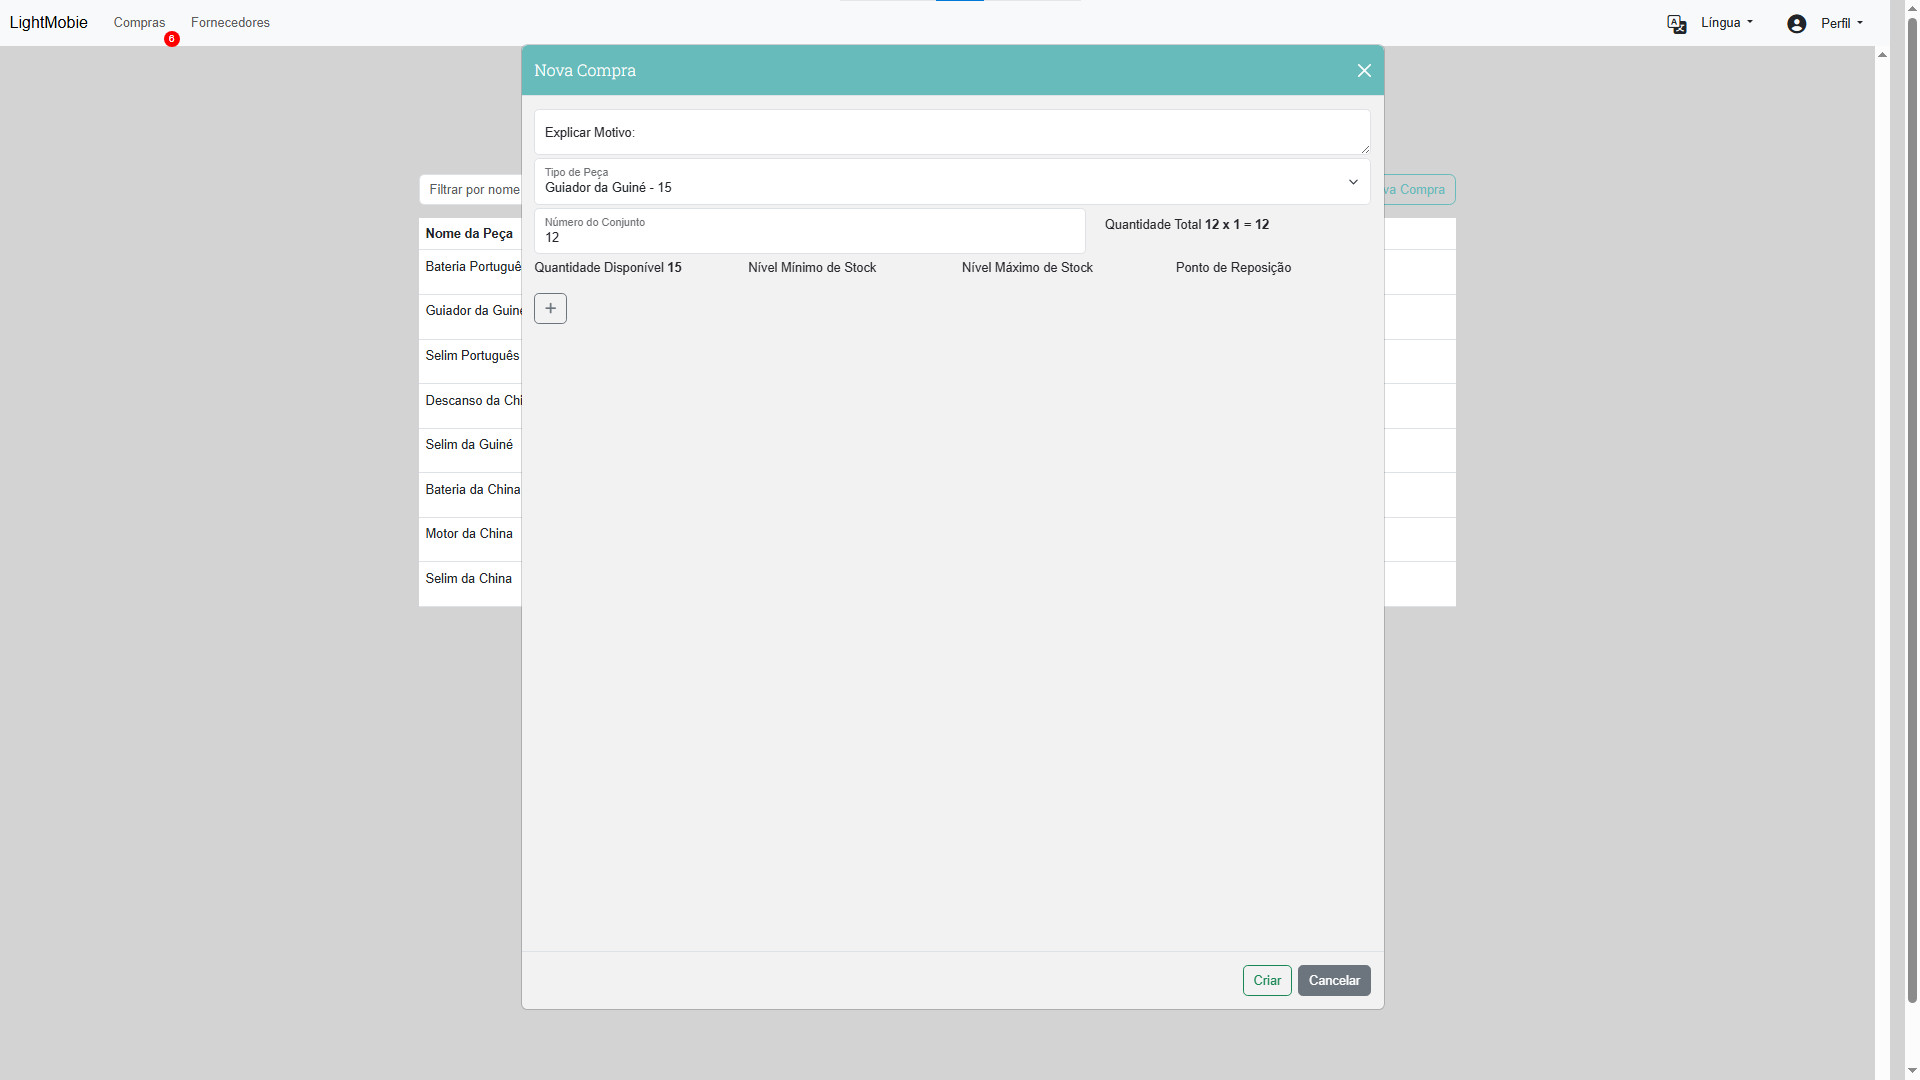
\includegraphics[width=\textwidth]{figs/Implementation/warehouse/createPurchaseWithParts}
  \label{fig:figure2}
\end{figure}

\begin{figure}[h]
  \caption{Create new purchase modal with a part added.}
  \centering
  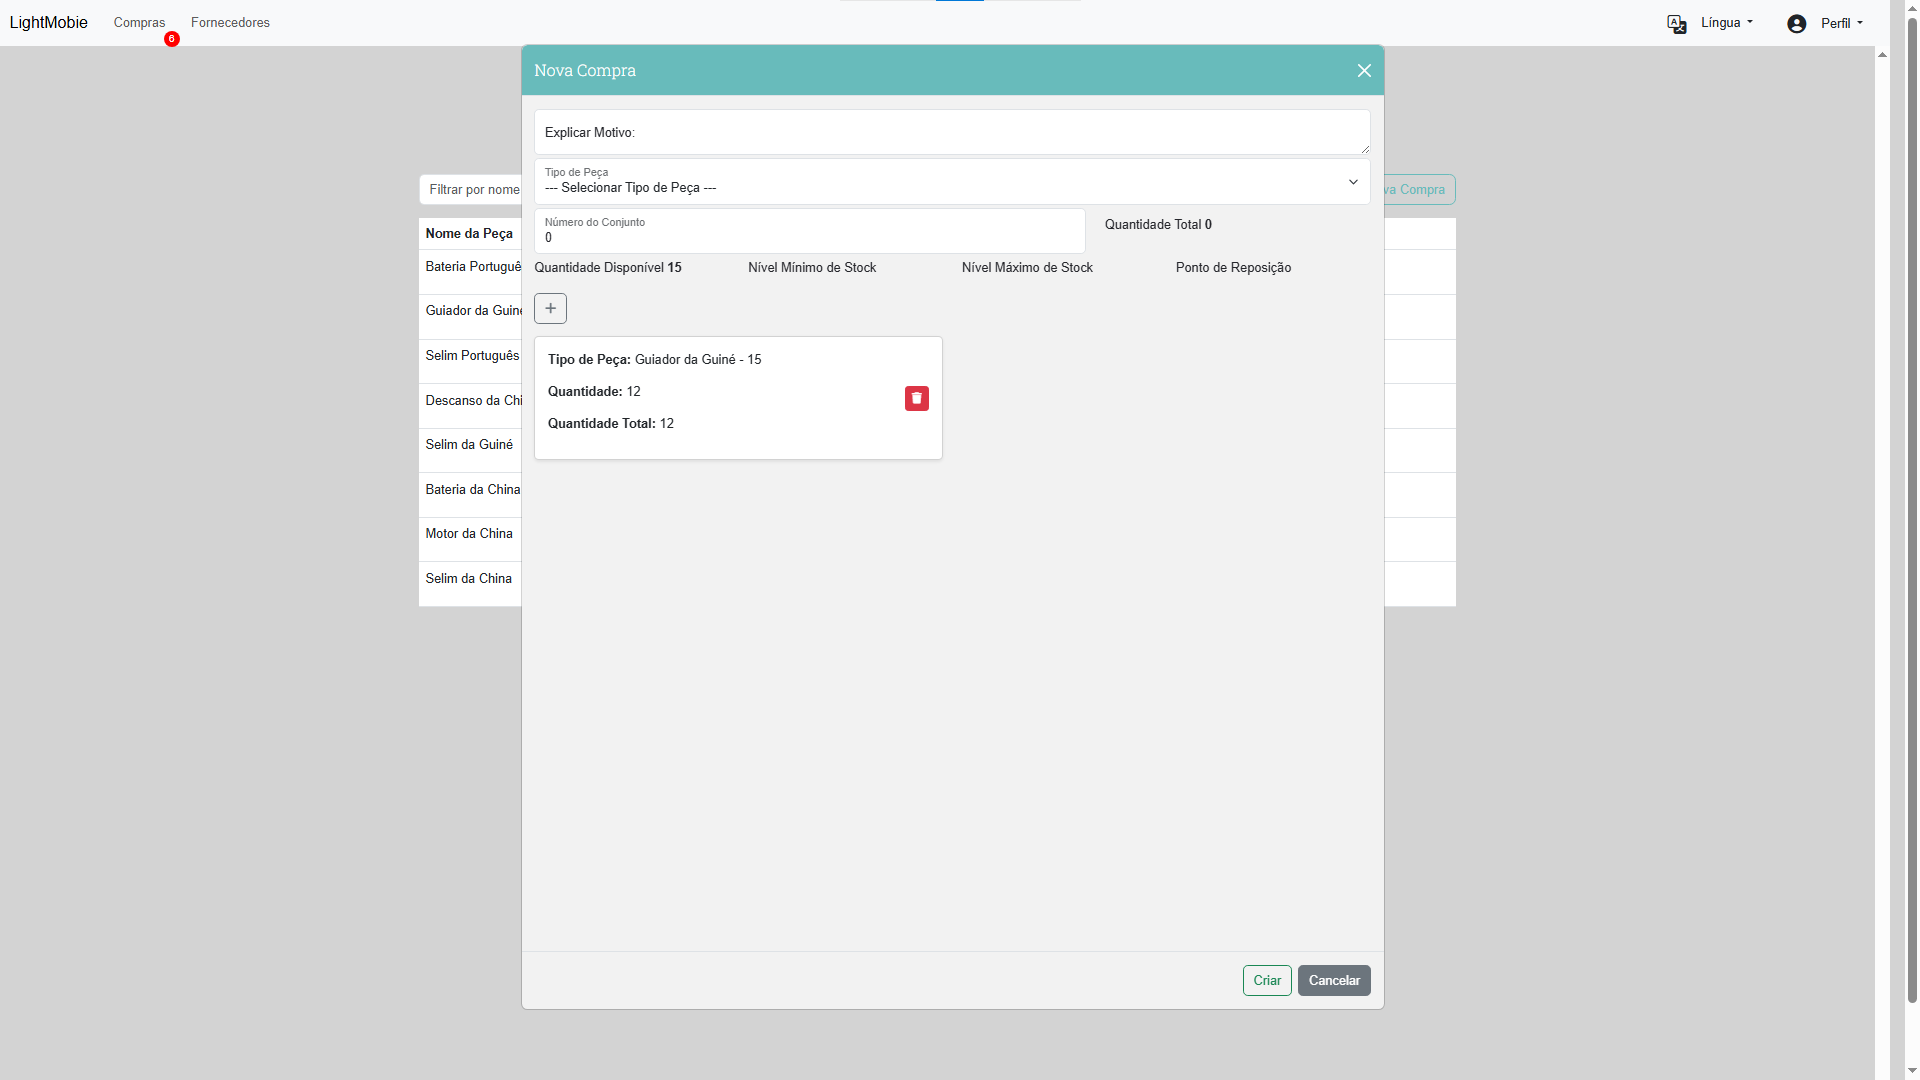
\includegraphics[width=\textwidth]{figs/Implementation/warehouse/createPurchaseAddedPart}
  \label{fig:figure2}
\end{figure}
In this modal, the warehouse operator can do the Use Case 3.2 – Requesting purchasing service , and , to accomplish that, he needs to fill a motive and choose which parts he wants to add to the purchase.
To add a part to the purchase he choses a part on the select (\ref), inserts the number of parts groups he wants to purchase, and clicks on the plus button.
After added a part he can add more, remove the part on the red button, or finish the purchase by clicking on the button "Criar" on the modal footer (\ref) .

\begin{figure}[h]
  \caption{List of purchases.}
  \centering
  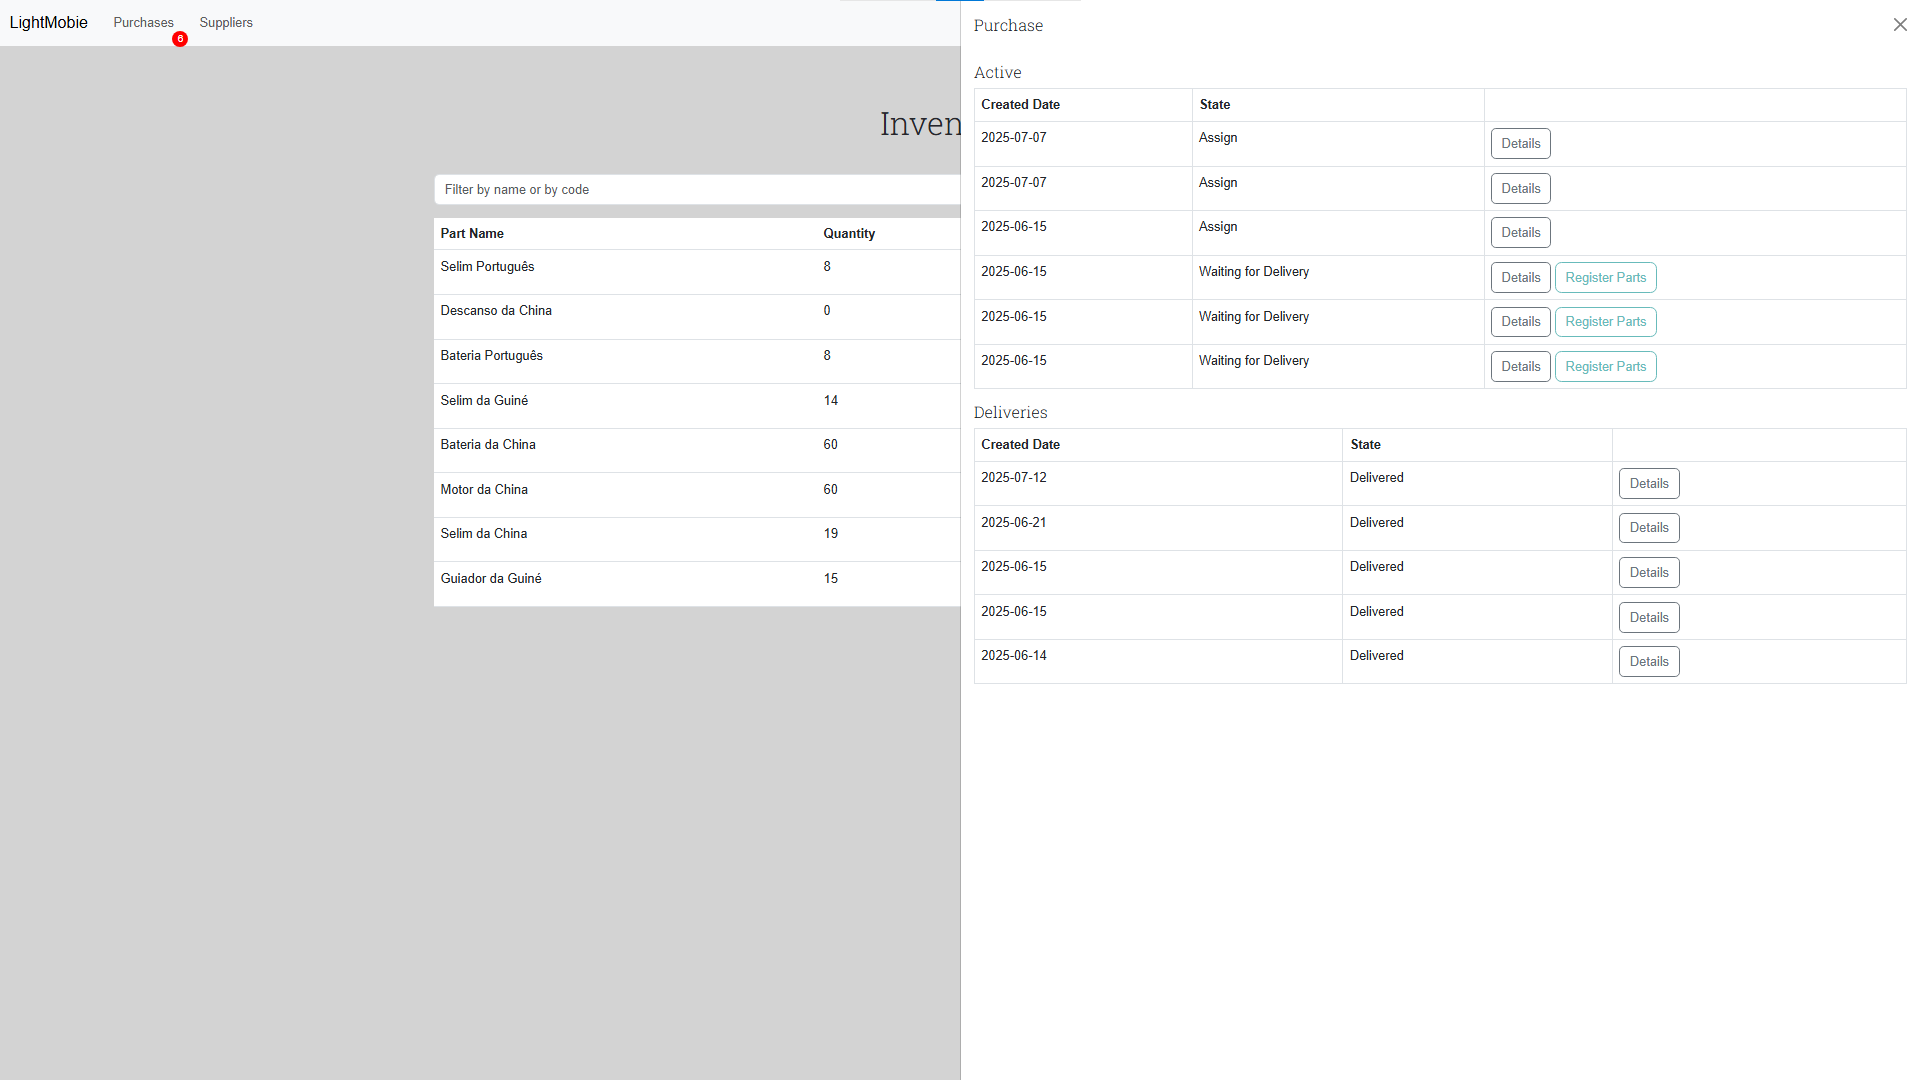
\includegraphics[width=\textwidth]{figs/Implementation/warehouse/PurchaseList}
  \label{fig:figure2}
\end{figure}


\begin{figure}[h]
  \caption{Assgined purchase details.}
  \centering
  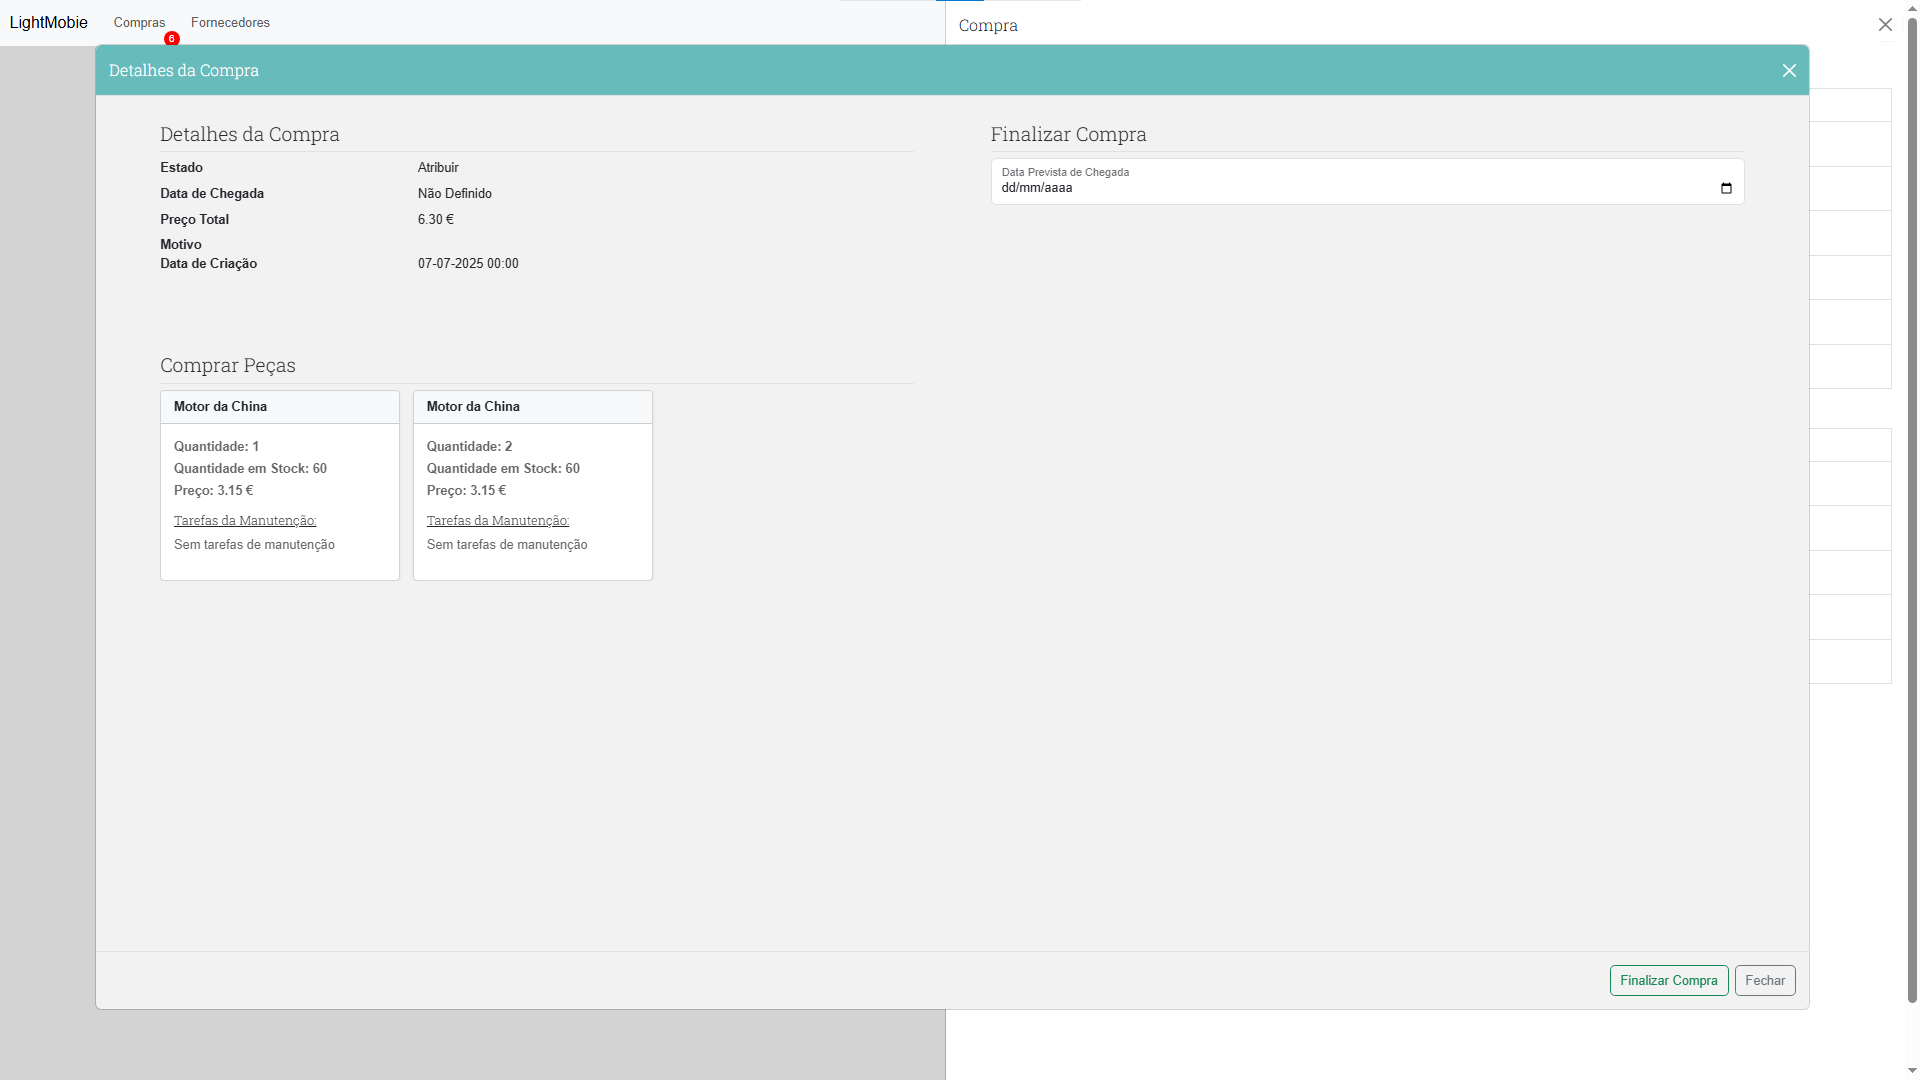
\includegraphics[width=\textwidth]{figs/Implementation/warehouse/PurchaseDetails}
  \label{fig:figure2}
\end{figure}

Returning to the home page, the warehouse operator may click on the button "Compras" on the menu and will open the list of purchases of the warehouse, as seen in \ref.
In this offcanvas there is two lists, the finished purchases and the active purchases. 
Each purchase has two type of information, the creation date and the status.
When clicking the details of a assigned purchase, it will open a modal like \ref.
In this modal the user can see the information about the purchase and finalize the purchase by assigning an expected arrival date.
The information provided is:
- the state of the purchase
- the arrival date
- the total price
- the motive of the purchase
- the creation date
- the parts of the purchase with the quantity being purchased, it quantity in stock, the price and the tasks assigned to the purchase. It is important to show this information to negotiate with the supplier to get the parts before the expected conclusion date of the maintenance.

\begin{figure}[h]
  \caption{Waiting delivery purchase details.}
  \centering
  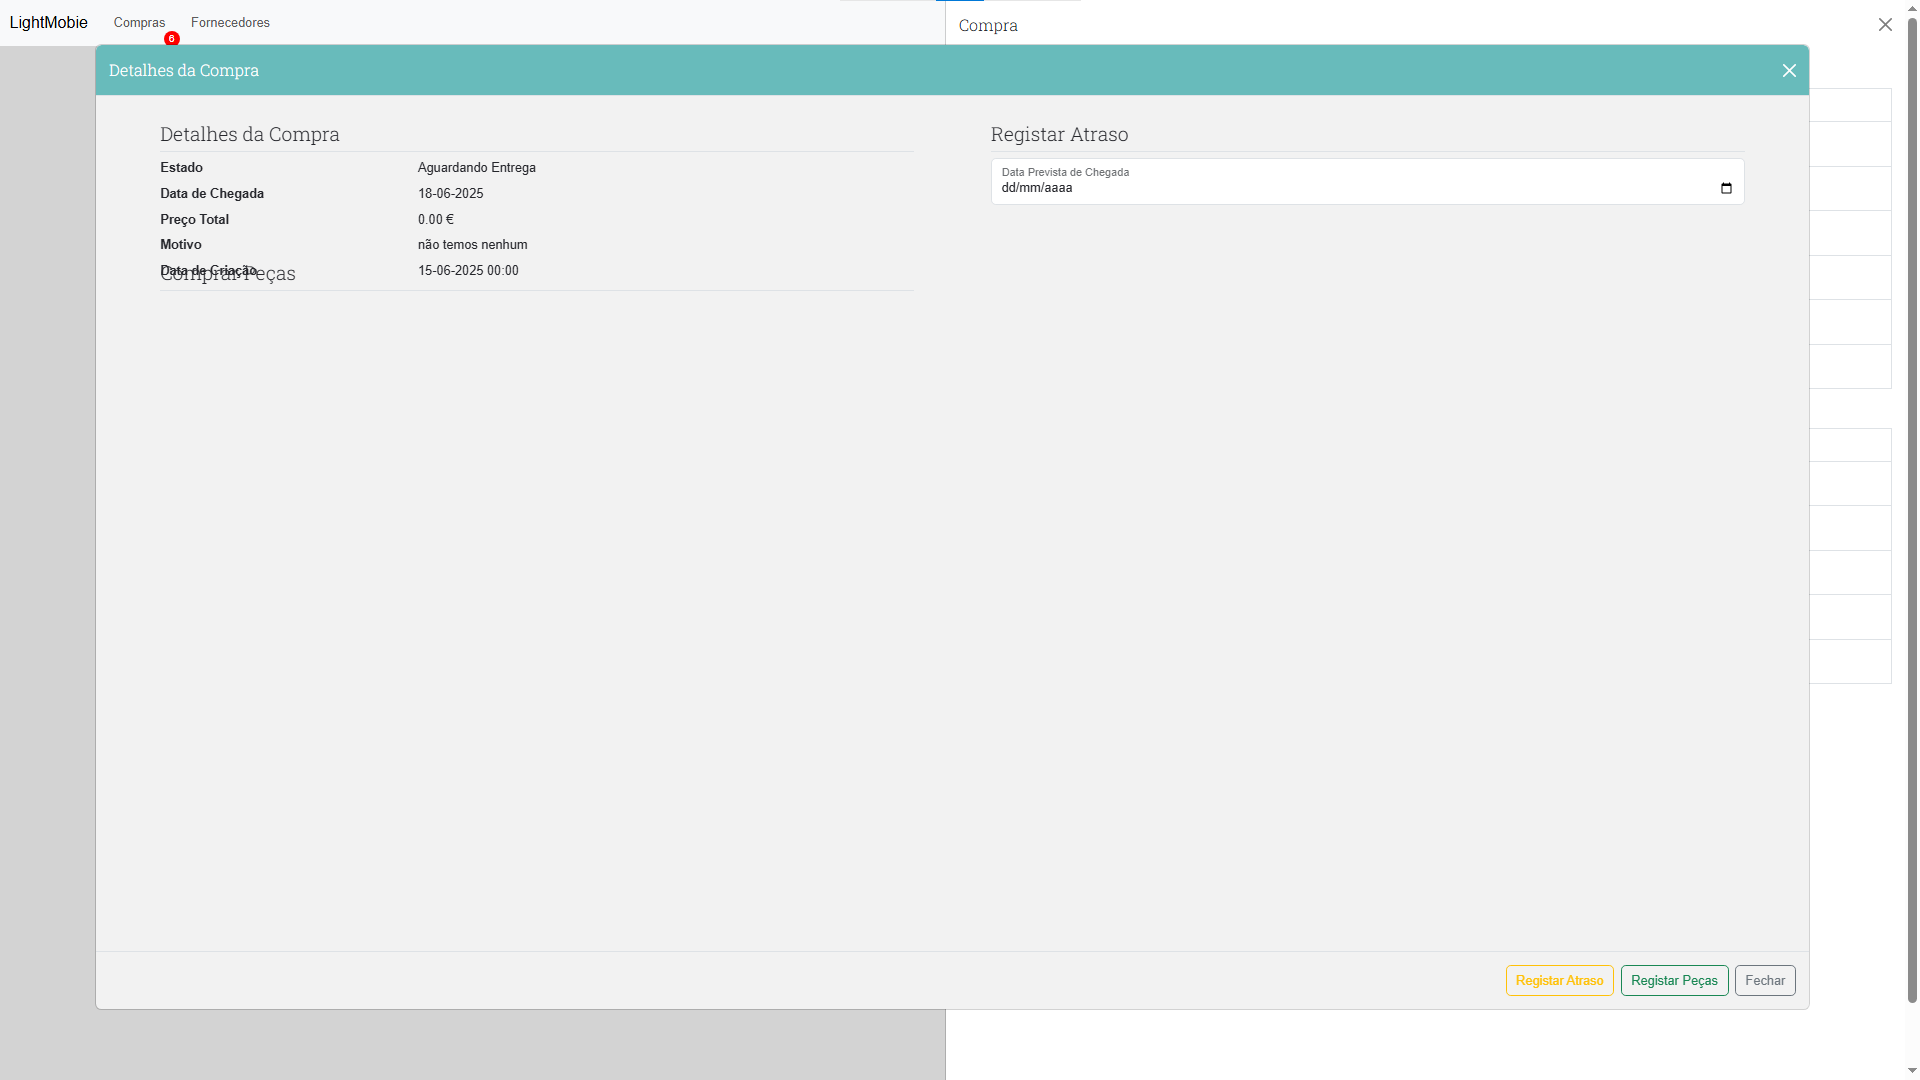
\includegraphics[width=\textwidth]{figs/Implementation/warehouse/PurchaseRegisterParts}
  \label{fig:figure2}
\end{figure}

If the user clicks on a waiting delivery purchase, the user can see the same information about the task, but also can add a purchase delay by adding a new expected arrival date; accomplising the Use Case 3.6 – Create Purchase Delay; or register the parts by clicking the "Registar peças" on the modal footer; accomplish the Use Case 3.4 – Registration of new parts in the System (\ref). 
The use case 3.4 can be also accomplished in the purchase list by clicking the button "Registar peças".

\begin{figure}[h]
  \caption{Delivered purchase details.}
  \centering
  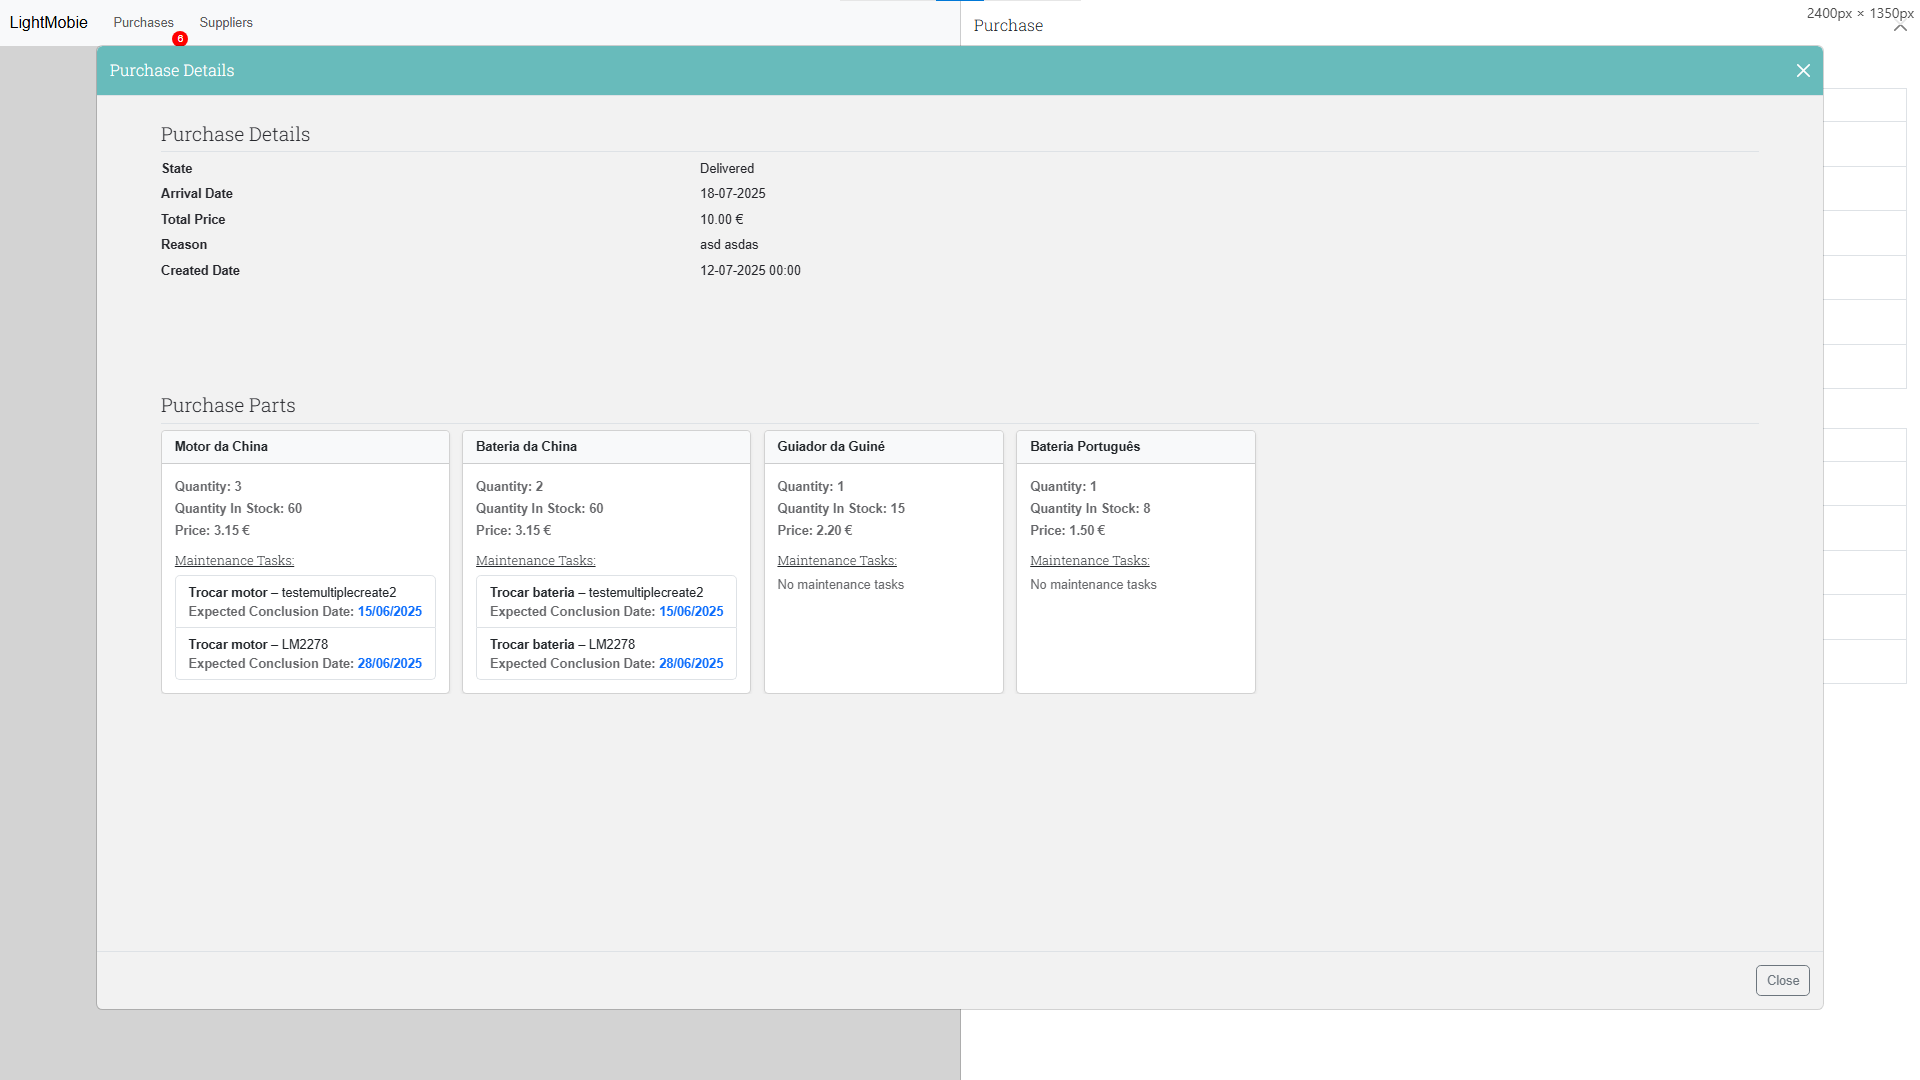
\includegraphics[width=\textwidth]{figs/Implementation/warehouse/PurchaseFinishedDetails}
  \label{fig:figure2}
\end{figure}
If the user clicks on the details of a delivered purchase, it will show the same kind of information as seen in \ref.


\begin{figure}[h]
  \caption{Supplier list.}
  \centering
  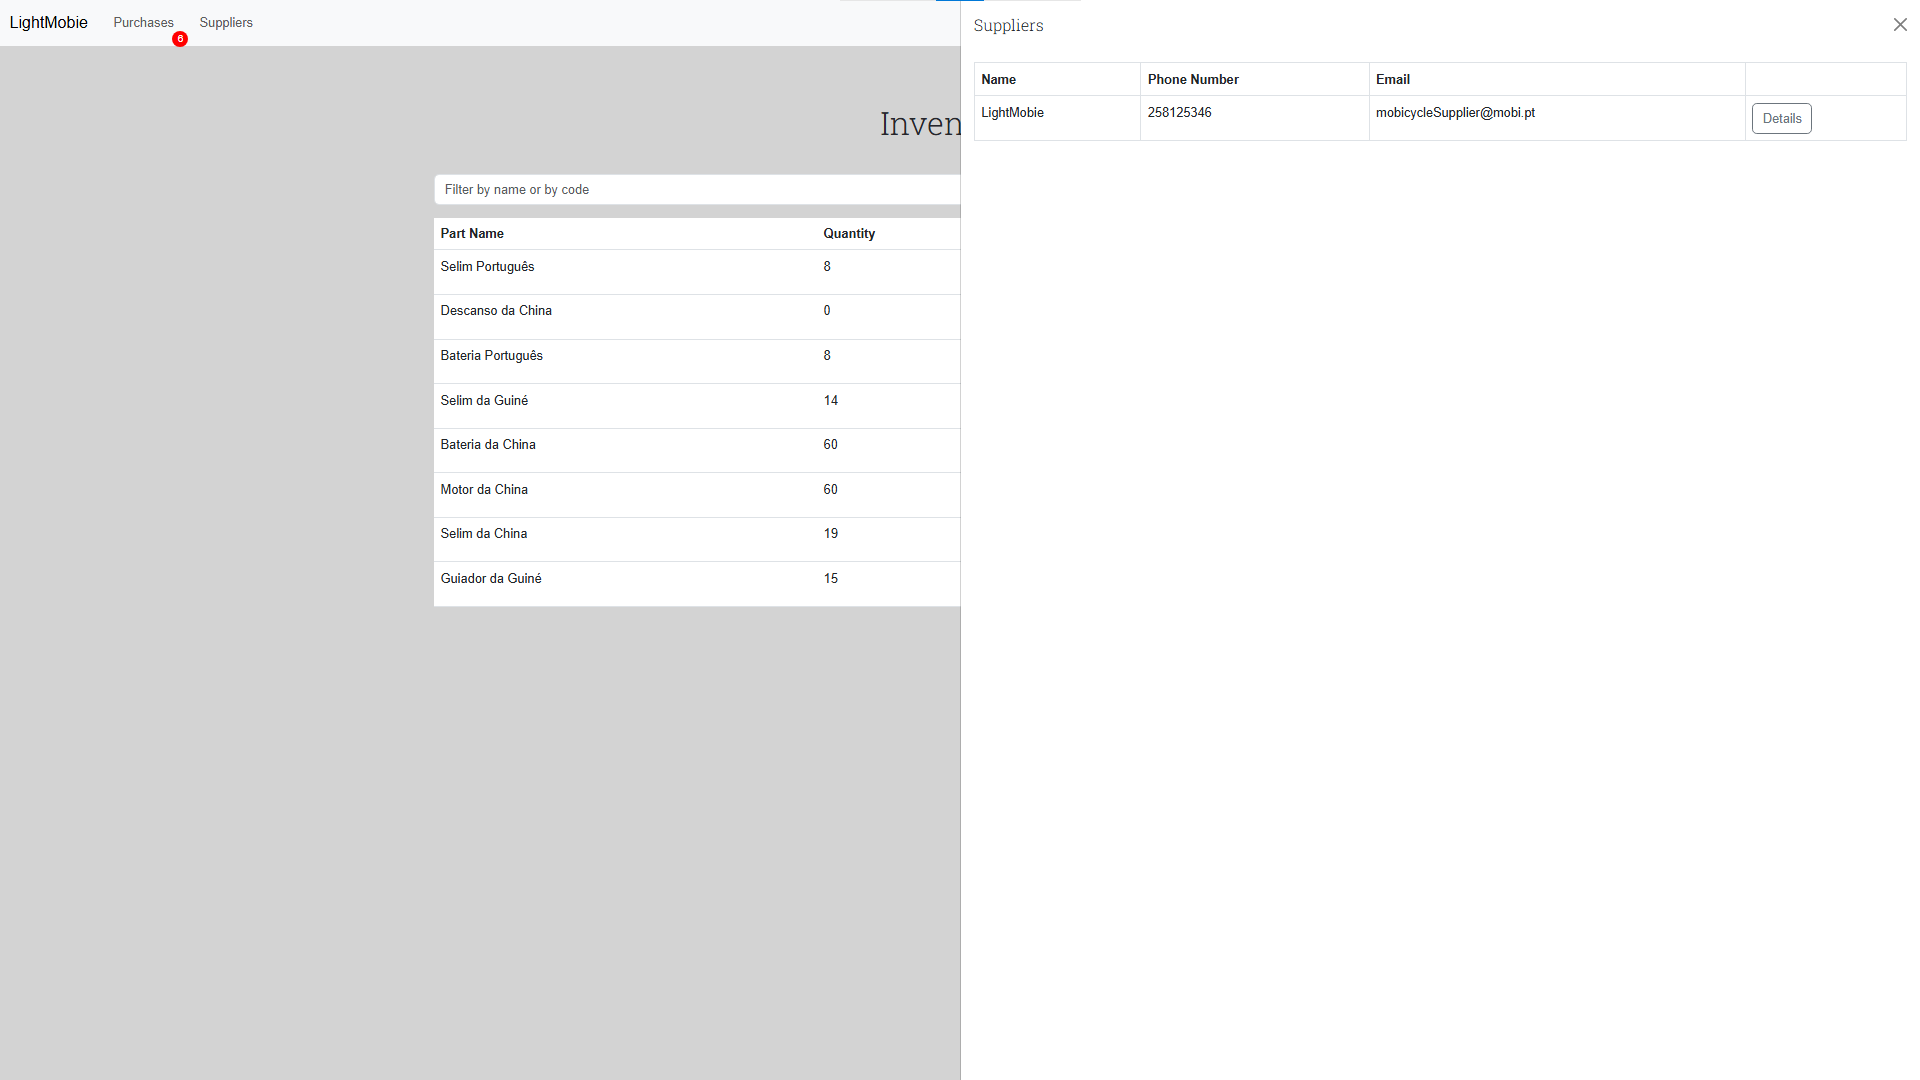
\includegraphics[width=\textwidth]{figs/Implementation/warehouse/supplierList}
  \label{fig:figure2}
\end{figure}

Returning to the home page the warehouse operator can also see the warehouse supplier by clicking on the button "Fornecedores" on the menu.
This will open a offcanvas, like the purchase, that will show a list of the supplier, as seen in \ref
This supplier has the following info:
- the name
- the Phone Number
- and the email

\begin{figure}[h]
  \caption{Supplier details.}
  \centering
  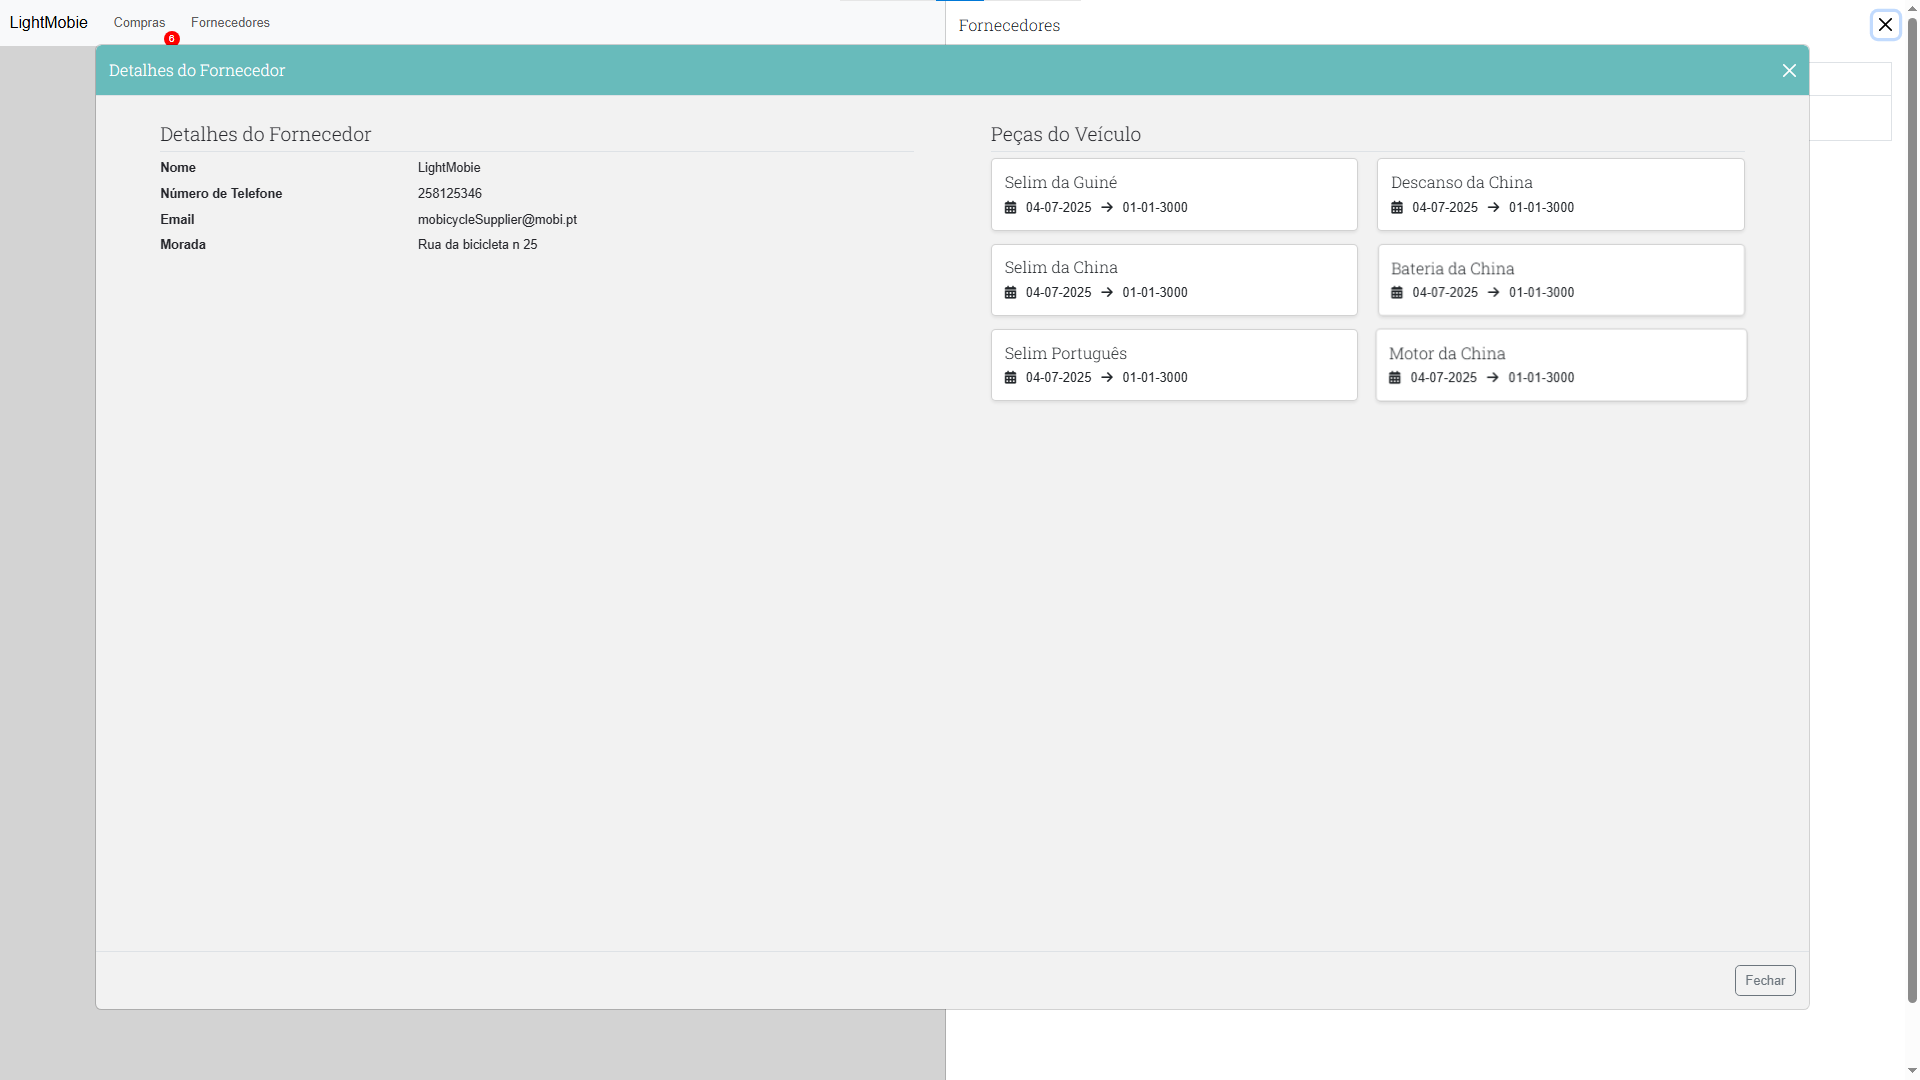
\includegraphics[width=\textwidth]{figs/Implementation/warehouse/supplierDetails}
  \label{fig:figure2}
\end{figure}

By clicking the details, it will show the same information plus the address of the supplier and the parts the supplier supplies (\ref).
Each part has the duration of the contract in which the supplier may supply the warehouse and the quantity of that.

\subsection{Workshop Manager view}

\begin{figure}[h]
  \caption{Workshop manager home page.}
  \centering
  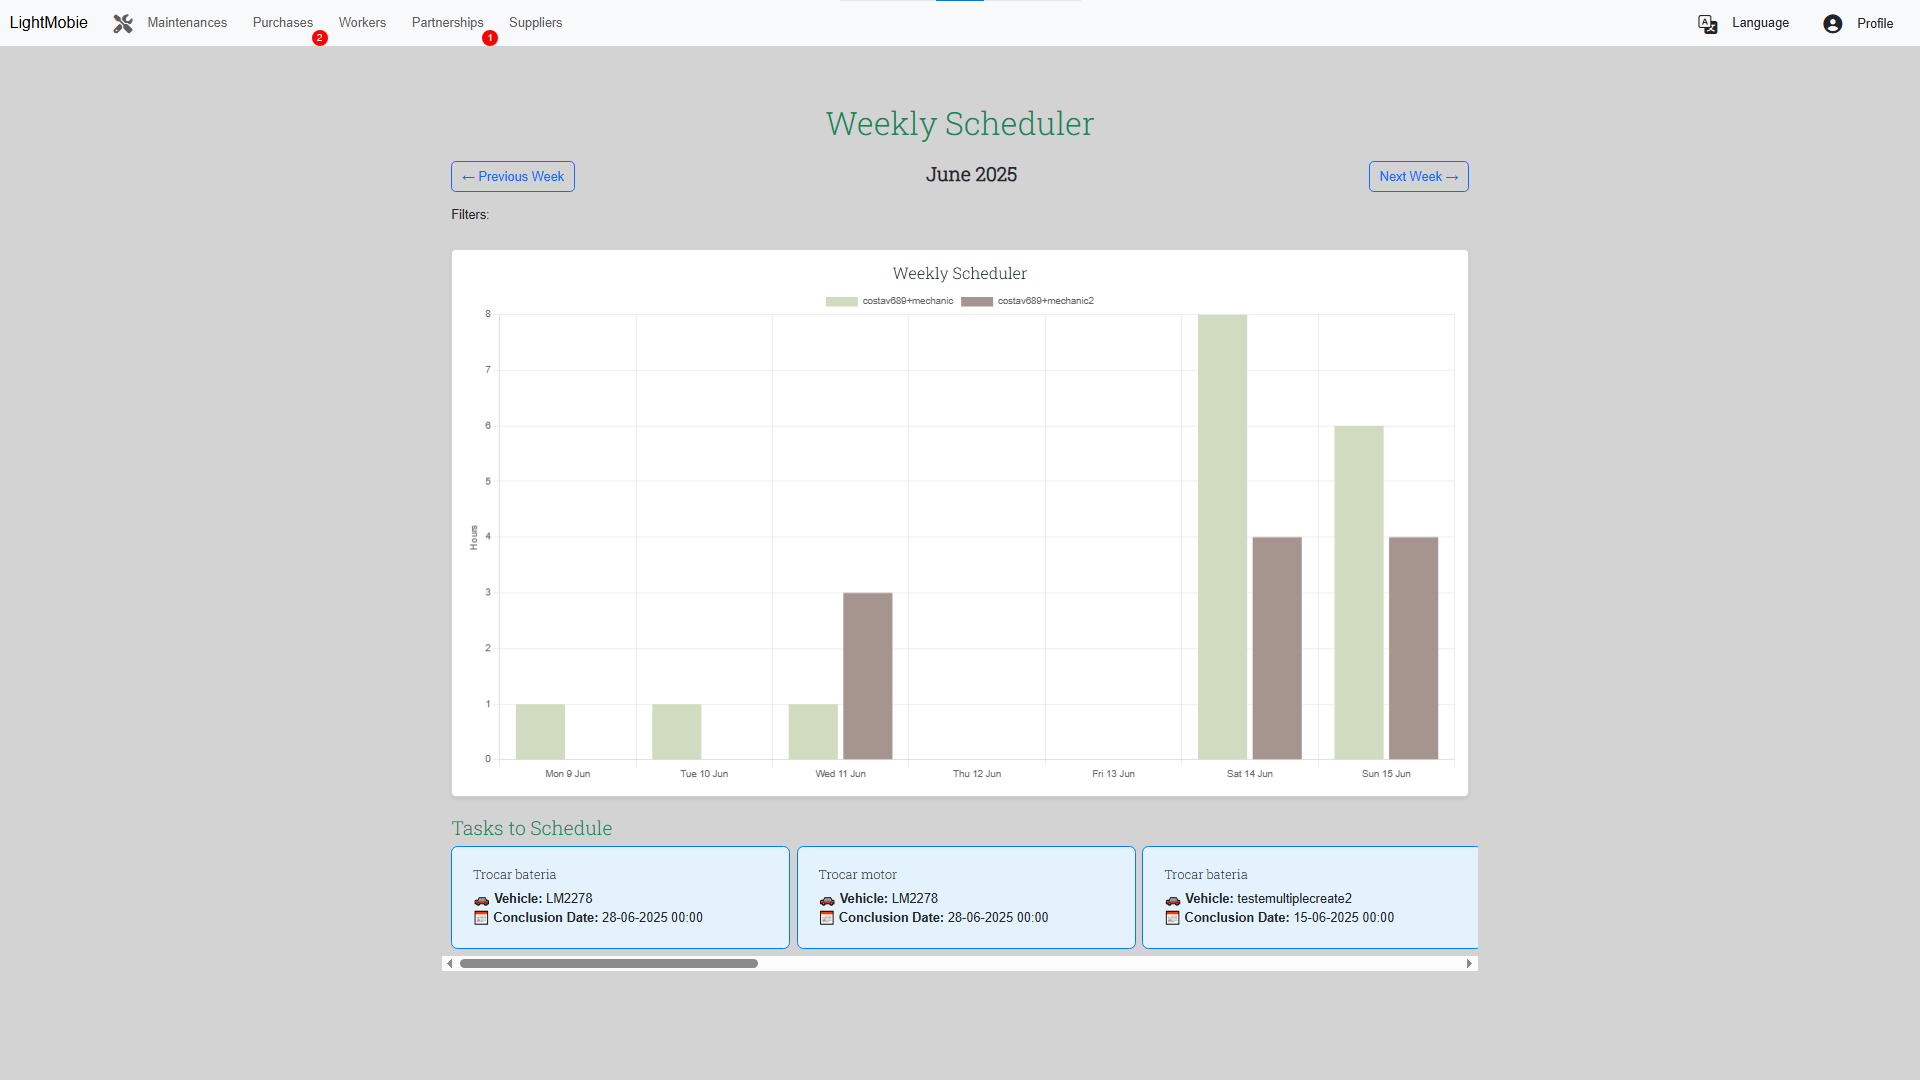
\includegraphics[width=\textwidth]{figs/Implementation/workshopmanager/homePage}
  \label{fig:figure2}
\end{figure}

The workshop manager view shows the general info of system.
The home page, as seen in \ref, is very similar to the rececionist where it is seen a graph with the tasks of the mechanics for a week. 
It differs by the column listing the tasks with no user assigned.
The manager can assigned a task on a user by clicking on a day in the graph or clicking on the button "Adicionar Task" and navegate to the day he wishes.
This action will open a modal with the details of the day as seen in \ref.

\begin{figure}[h]
  \caption{Assign task to a mechanic.}
  \centering
  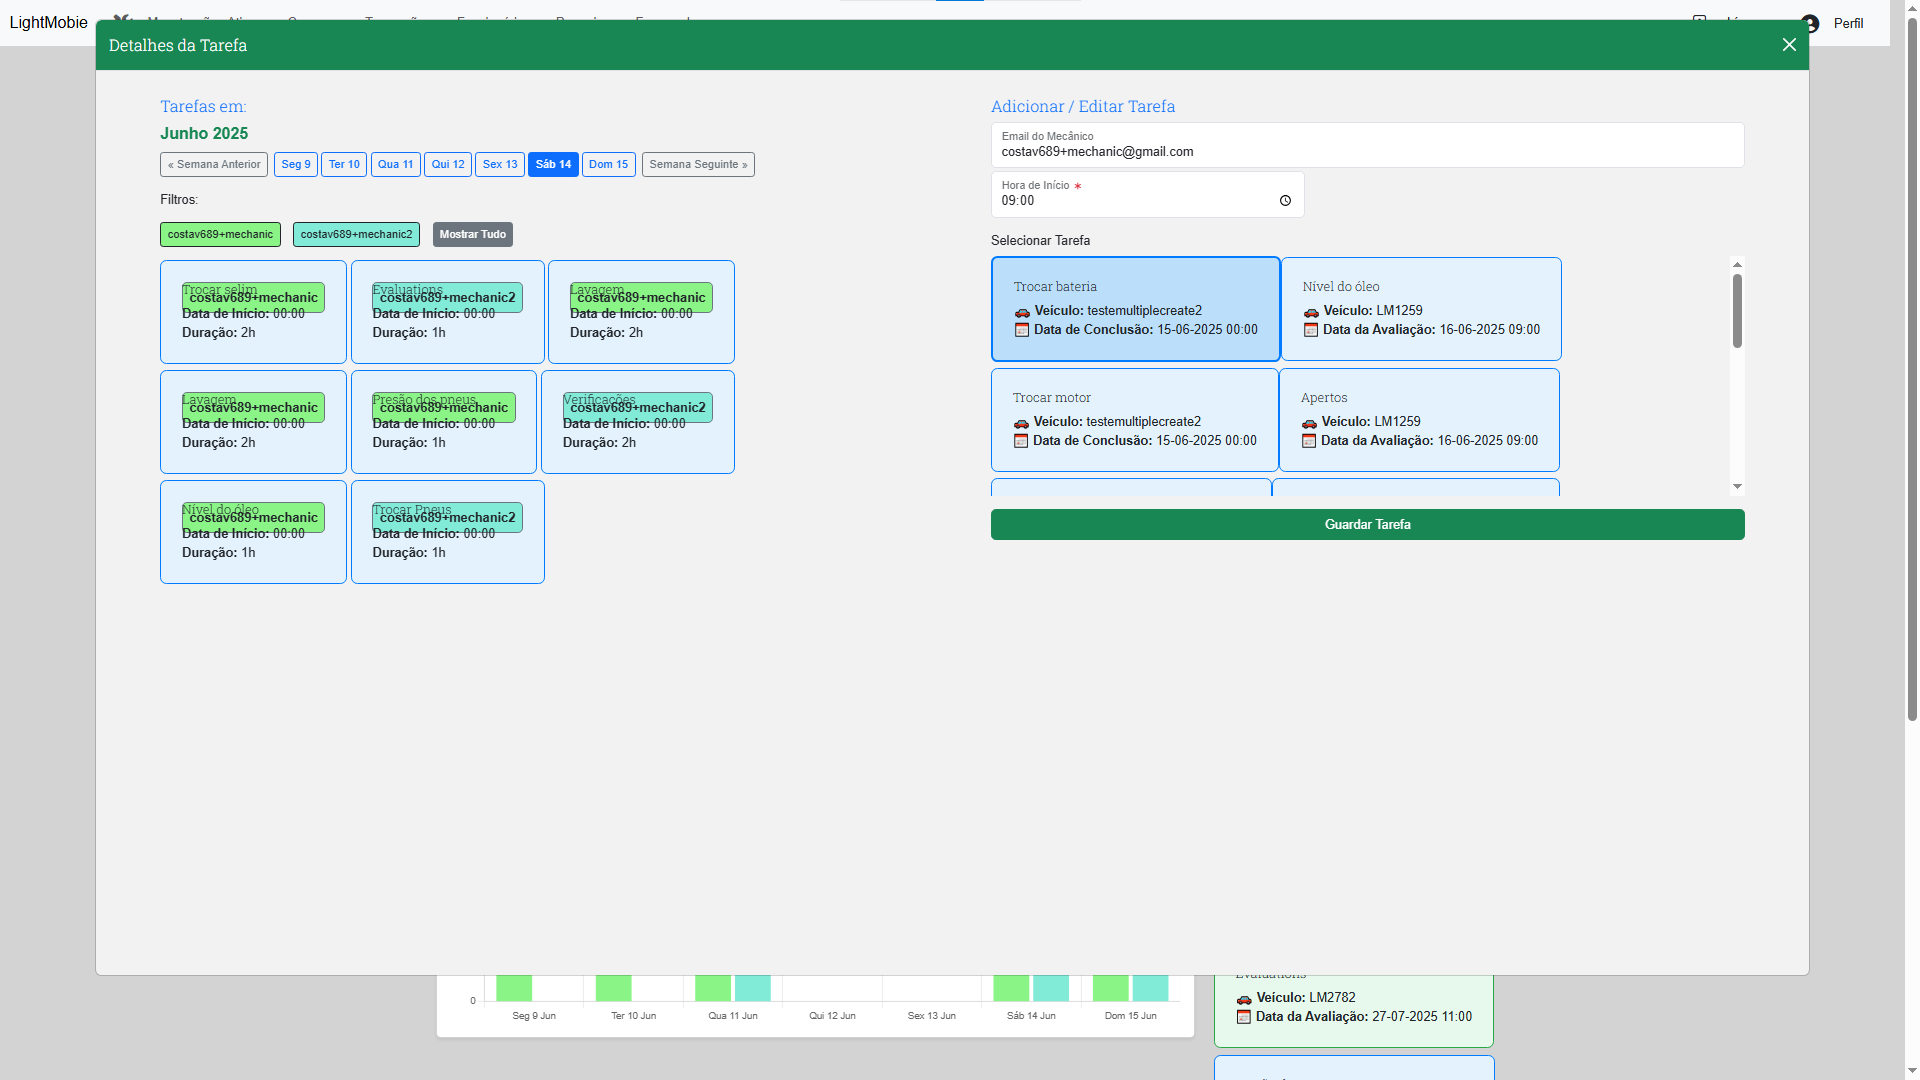
\includegraphics[width=\textwidth]{figs/Implementation/workshopmanager/addTask}
  \label{fig:figure2}
\end{figure}

This modal is also very similar as in the rececionist schedule task modal, but on the right is the form to assigned the task to a mechanic. 
To fill this form the manager must select the mechanic by writting their email, the hour he wants the task to begin (maybe remove this) and the task he wants to assigned to the user.

\begin{figure}[h]
  \caption{Active maintenance list.}
  \centering
  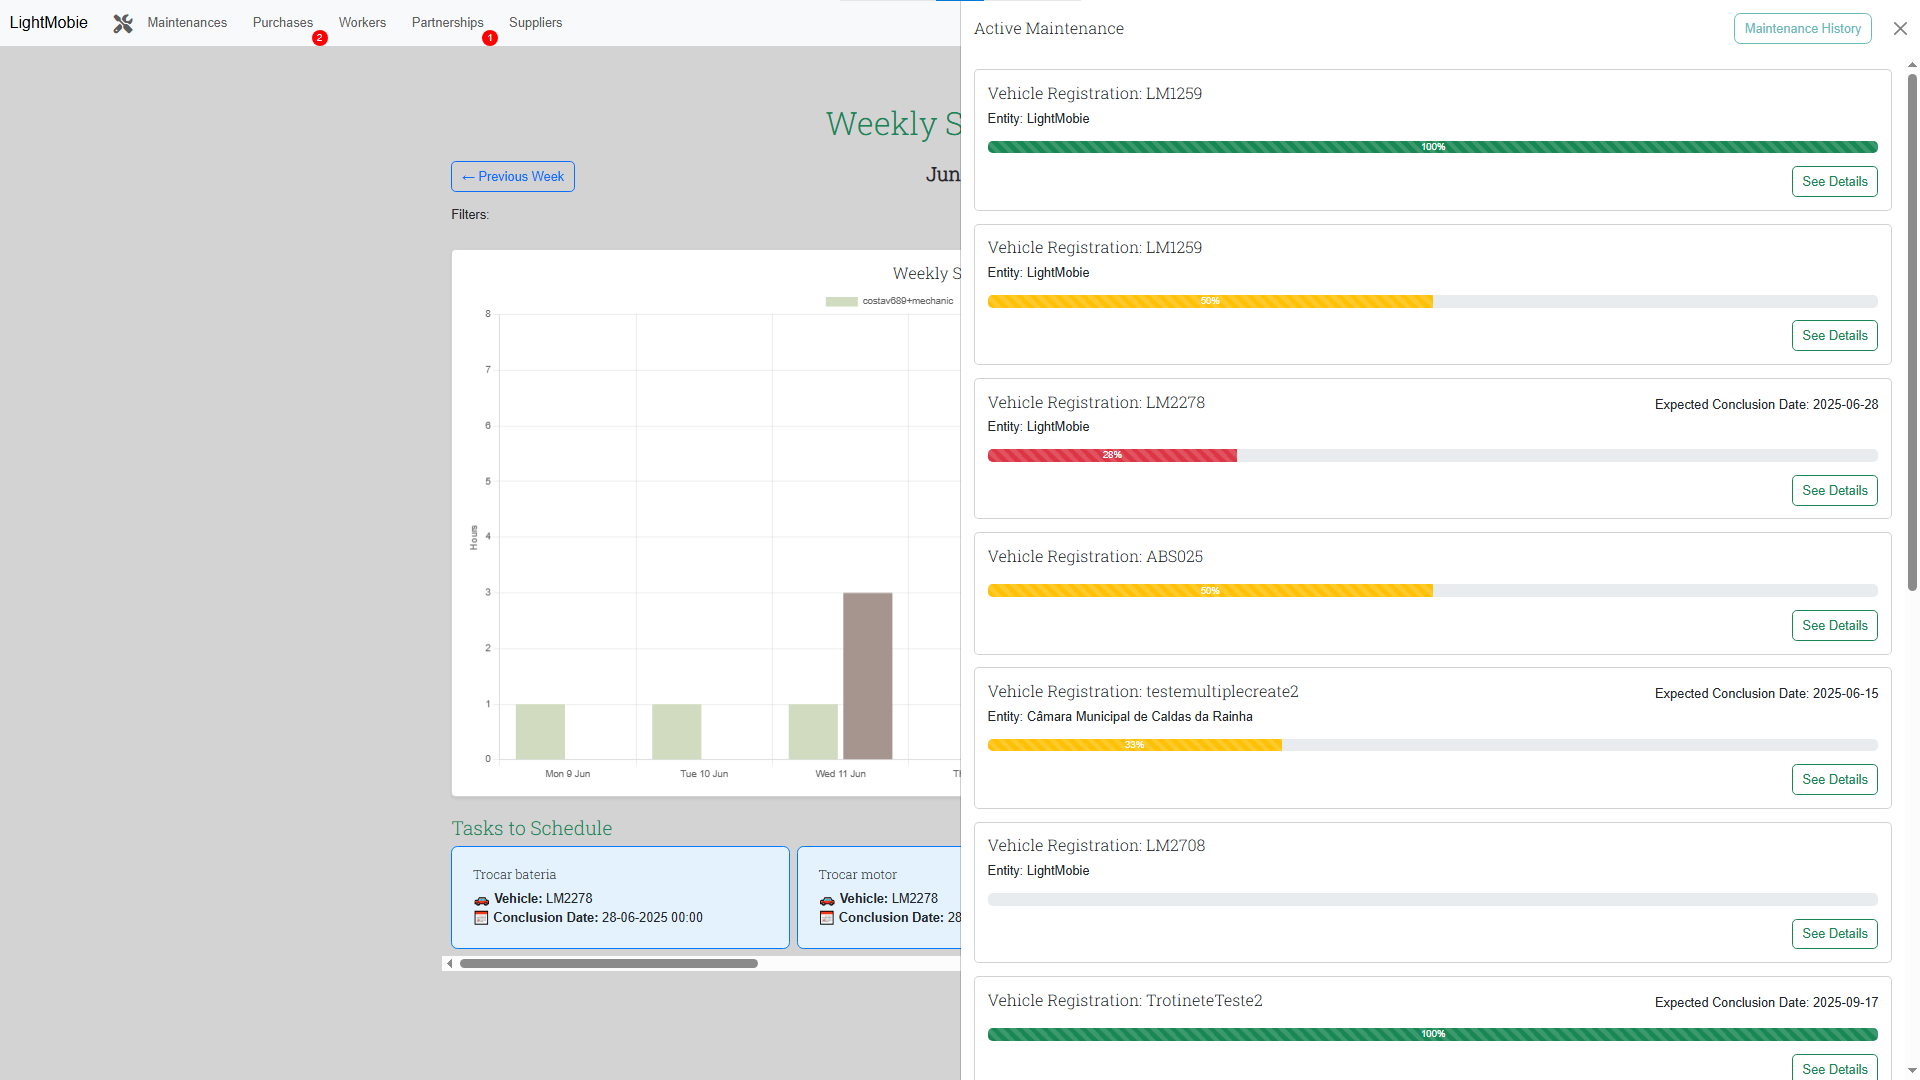
\includegraphics[width=\textwidth]{figs/Implementation/workshopmanager/maintenanceList}
  \label{fig:figure2}
\end{figure}


\begin{figure}[h]
  \caption{Maintenance details information tab.}
  \centering
  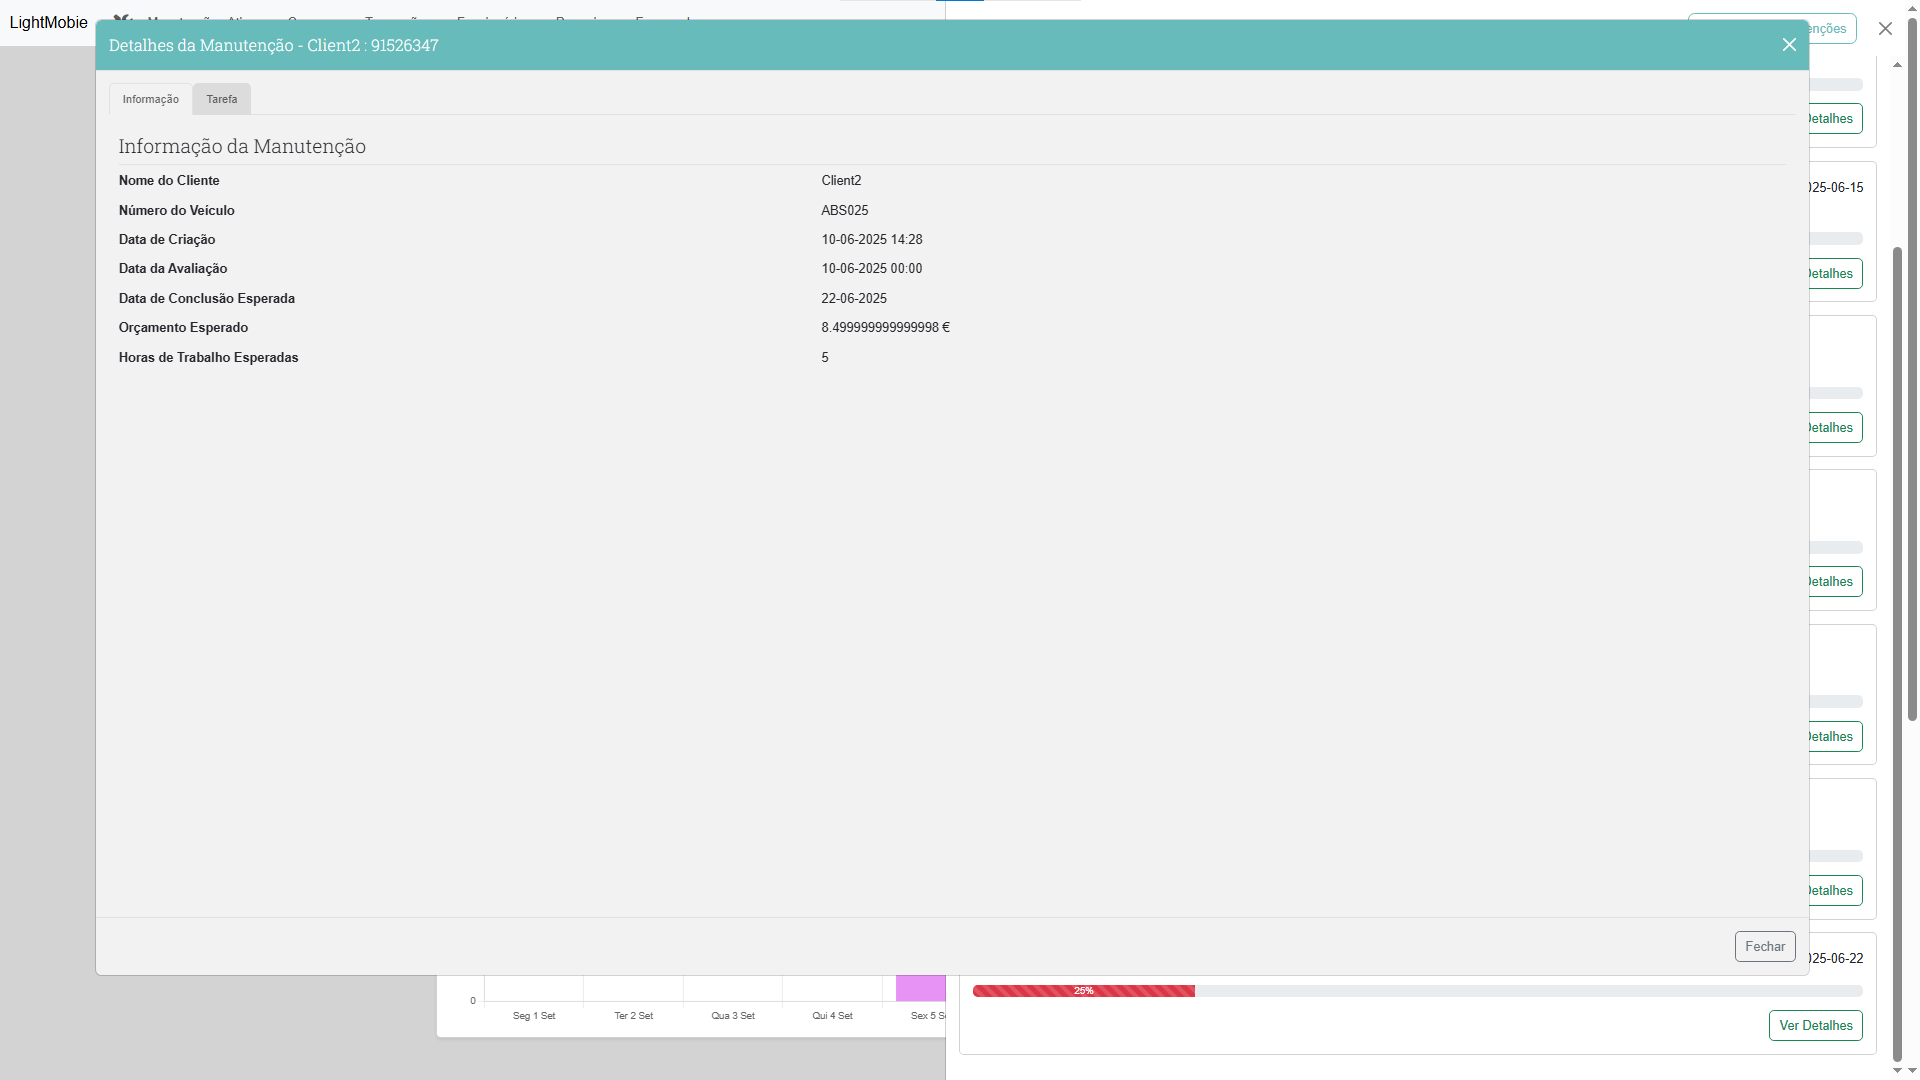
\includegraphics[width=\textwidth]{figs/Implementation/workshopmanager/maintenanceDetails}
  \label{fig:figure2}
\end{figure}

\begin{figure}[h]
  \caption{Maintenance details tasks tab.}
  \centering
  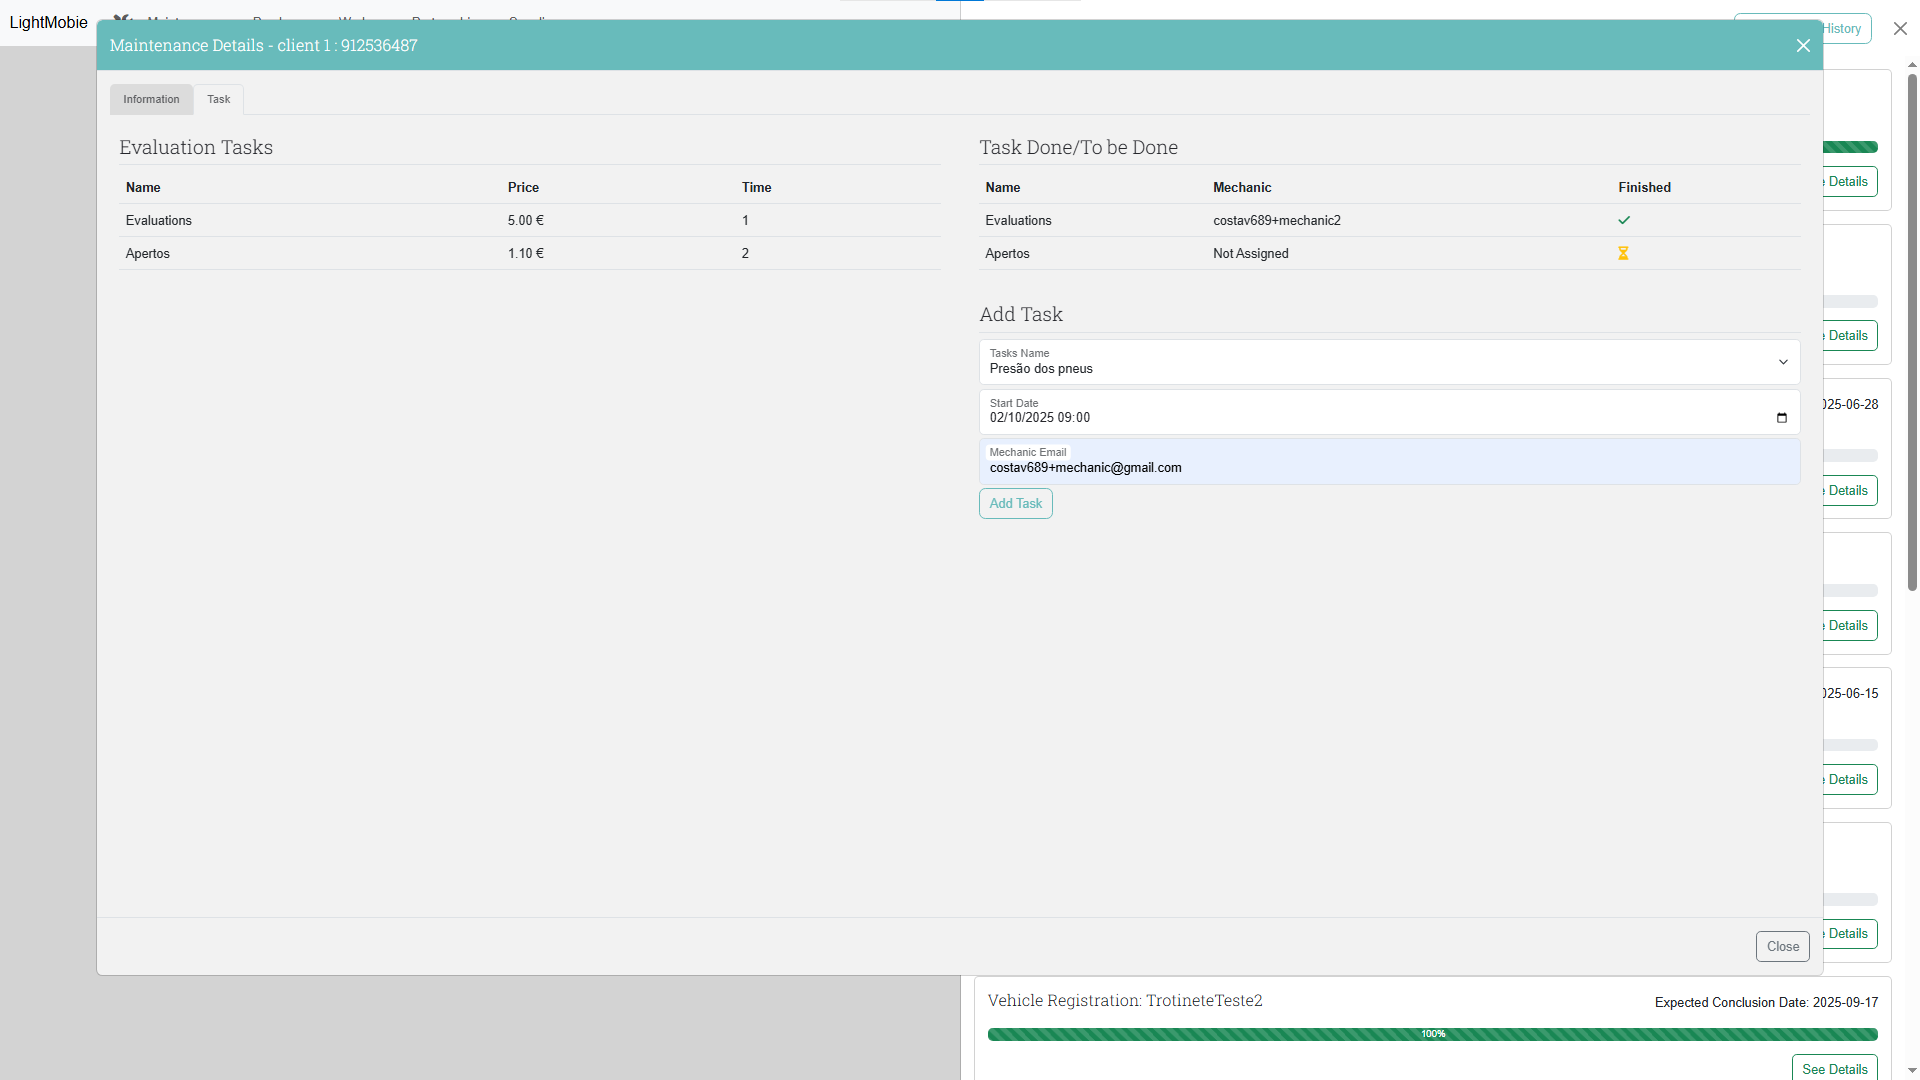
\includegraphics[width=\textwidth]{figs/Implementation/workshopmanager/maintenanceDetailsTask}
  \label{fig:figure2}
\end{figure}

Returning to the home page, the manager to see information about a maintenance may click on the button "Mutações ativas" on the menu.
This will show a offcanvas with the list of active maintenances, very similar as the rececionist, as wee can see in \ref.
This maintenance details show the same information as the rececionist, including the tasks tab, but doen't has the tab of the "alterações", as seen in \ref and \ref.
It has the additional funcionality of adding a task to a maitnenace on the task tab, to this the manager just needs to select the task, the mechanic and the date for the mechanic to do the task. 
This will provoke a maintenance change that needs to be validated by the client.

\begin{figure}[h]
  \caption{Maintenance history list.}
  \centering
  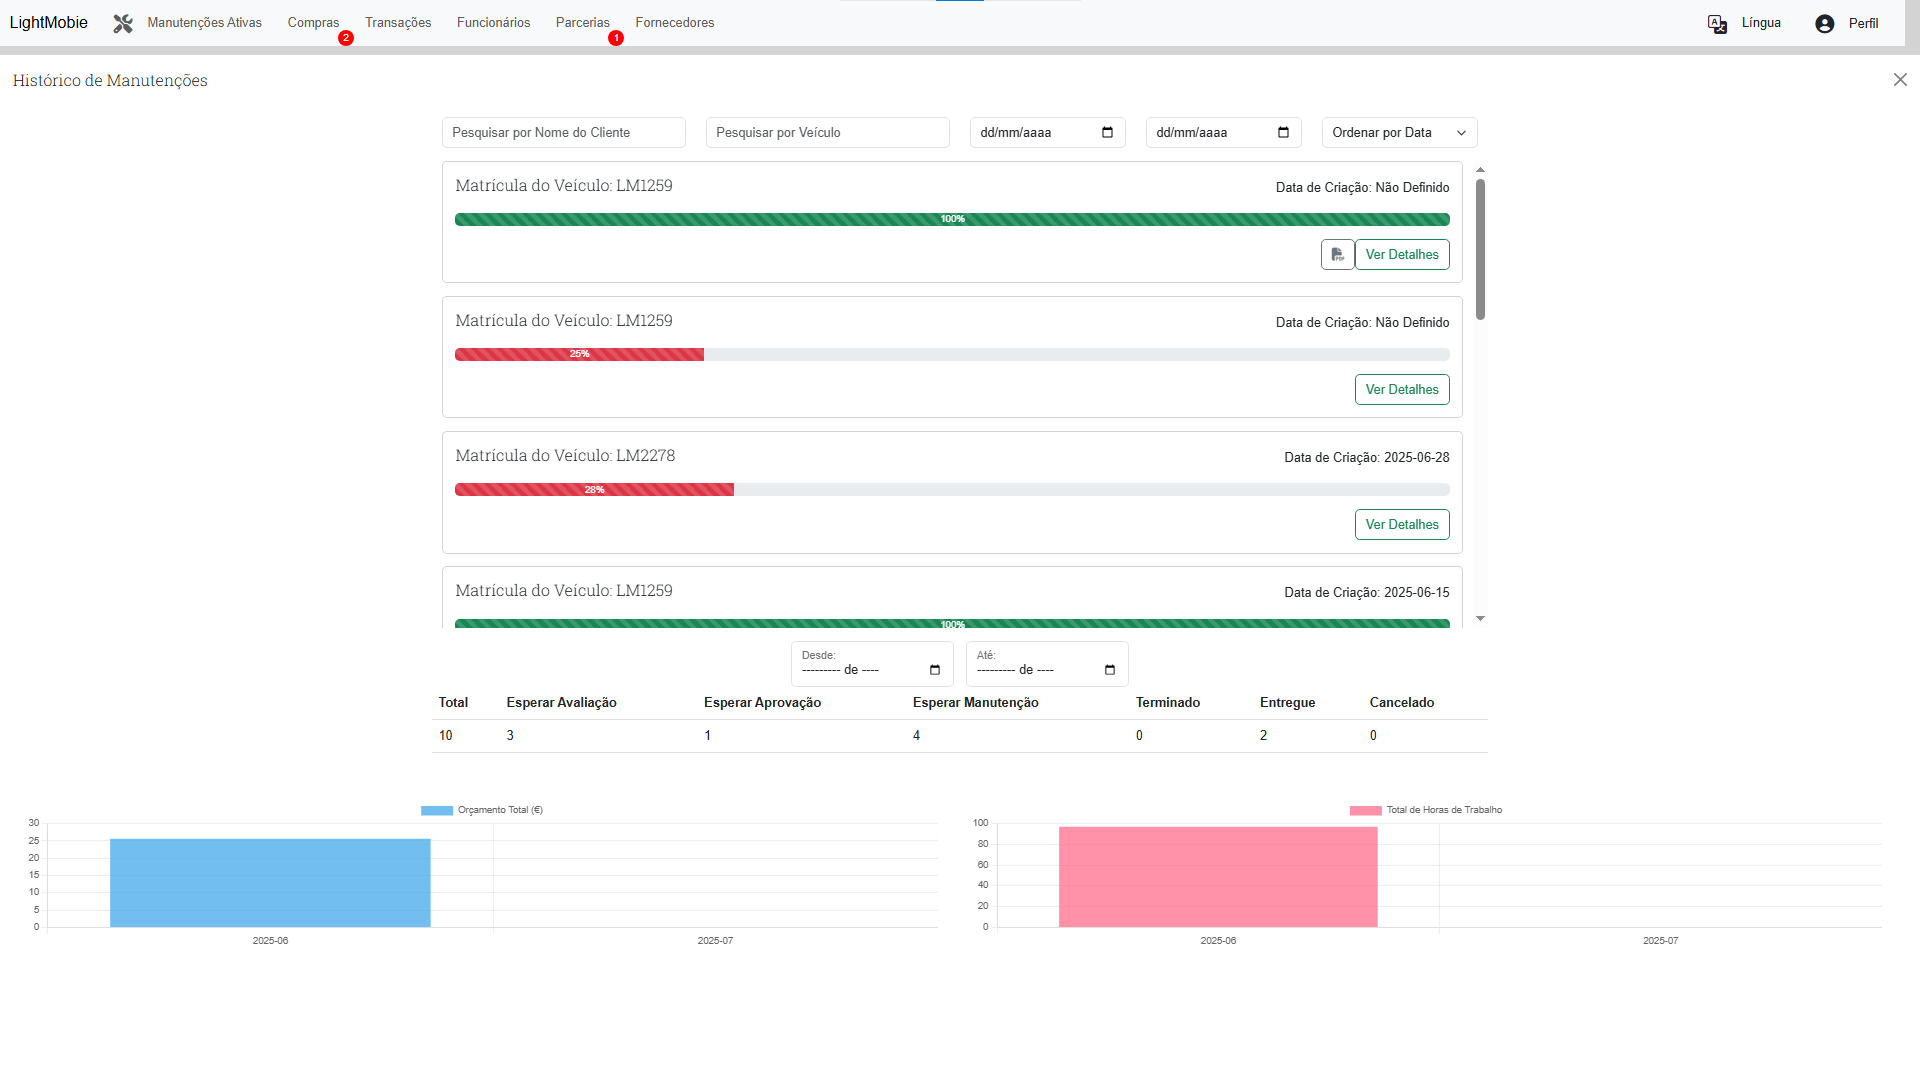
\includegraphics[width=\textwidth]{figs/Implementation/workshopmanager/maintenanceHistory}
  \label{fig:figure2}
\end{figure}

The offcanvas has the additional funcionally of showing the history of maintenance done by the dealership (Use Case 4.3 – View history of maintenance performed), by clicking in the button "Histórico de Manutenções" on the top of offcanvas.
This will open another offcanvas as seen in \ref.

\begin{figure}[h]
  \caption{Report example.}
  \centering
  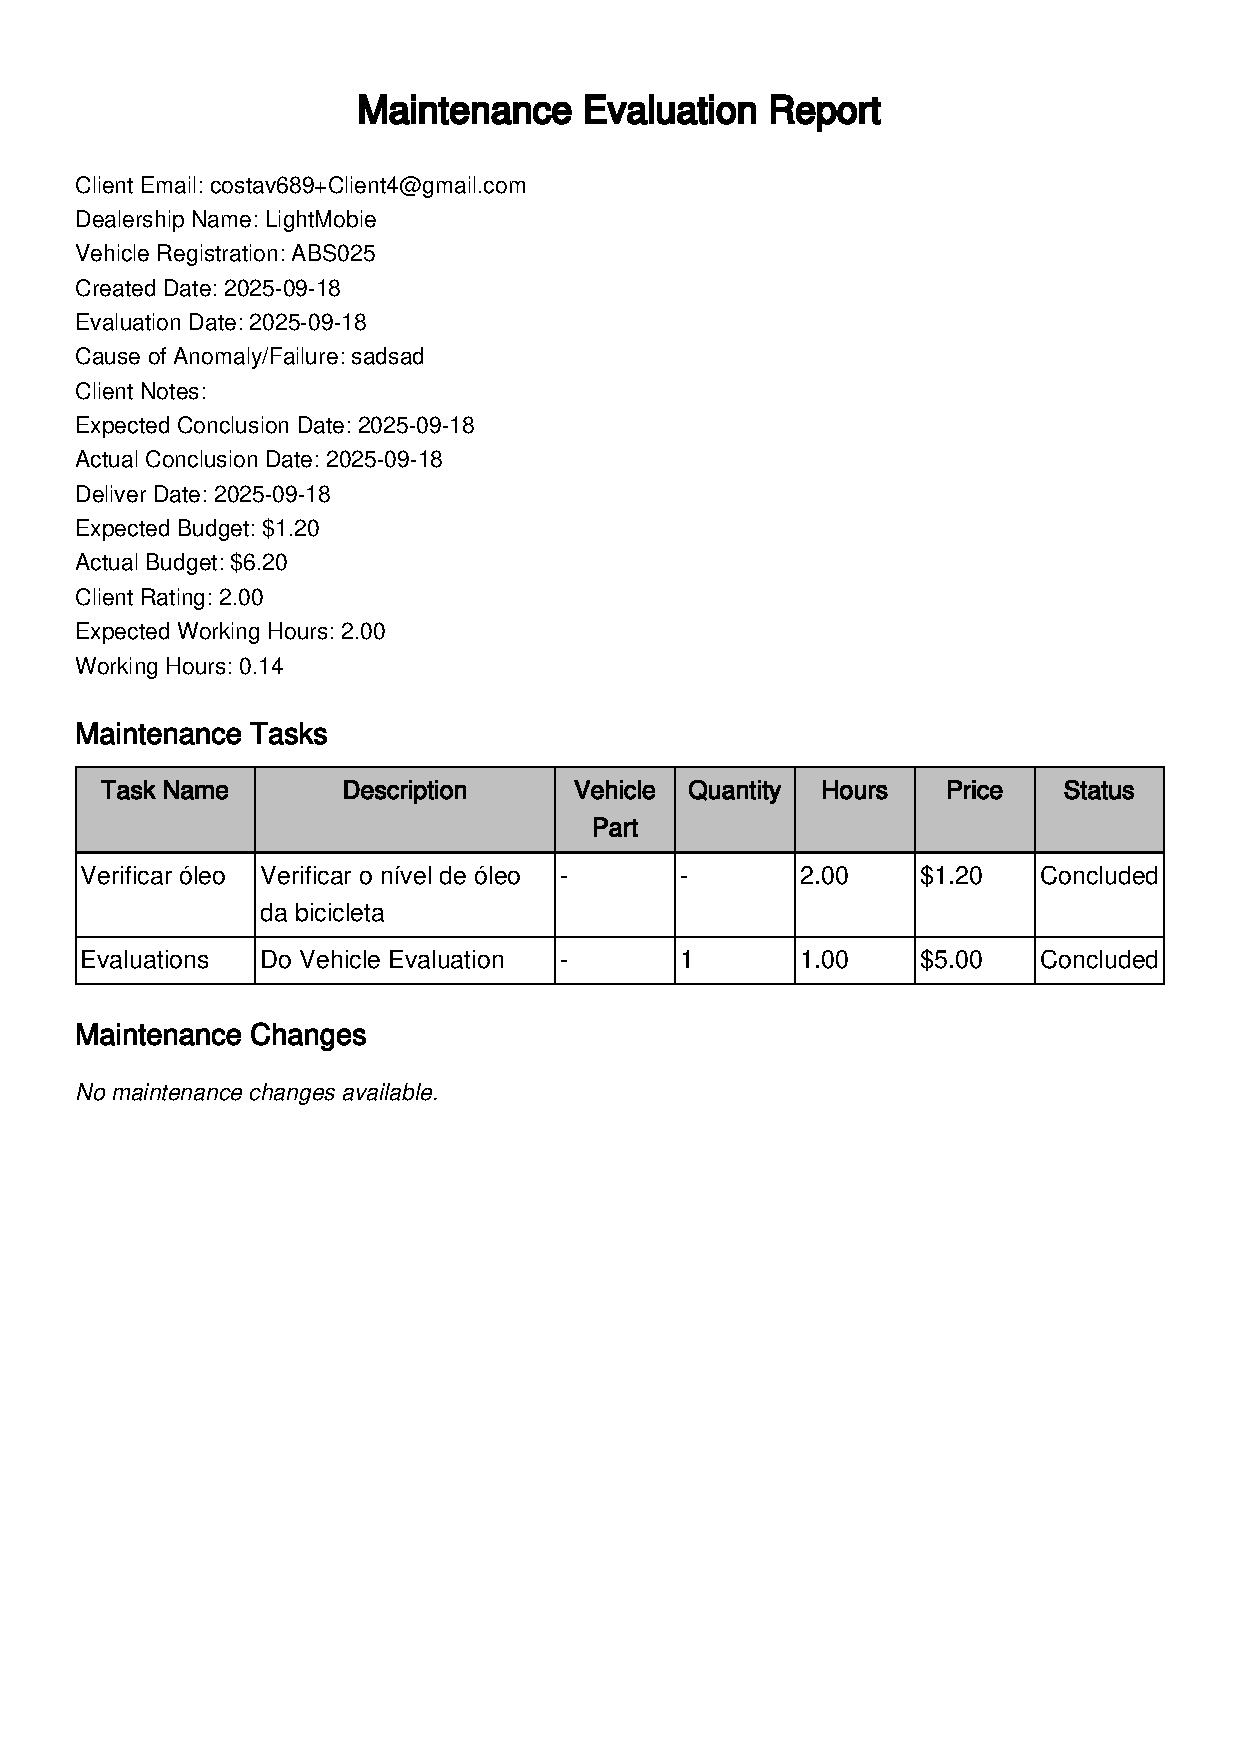
\includegraphics[width=\textwidth]{figs/Implementation/workshopmanager/report}
  \label{fig:figure2}
\end{figure}


In this offcanvas we can filter the list by client, vehicle registration, and date.
Each maintenance details will show the same modal as in the active maintenance list, but the maintenances that are concluded, the card has a button beside the "Ver Detalhes" with the icon of a pdf.
This button will return the report of the maintenance, that is the information of the maintenance in a report format. This report can be see in \ref. 
Below the list of maintenance there is some statistics about the maintenances (Use Case 4.4 – Develop statistics). 
First there is a table with the total number of maintenance in each state, and below two graphs:
- one with the total revenue per month, and the other the number of working hours per month


\begin{figure}[h]
  \caption{Purchase request list.}
  \centering
  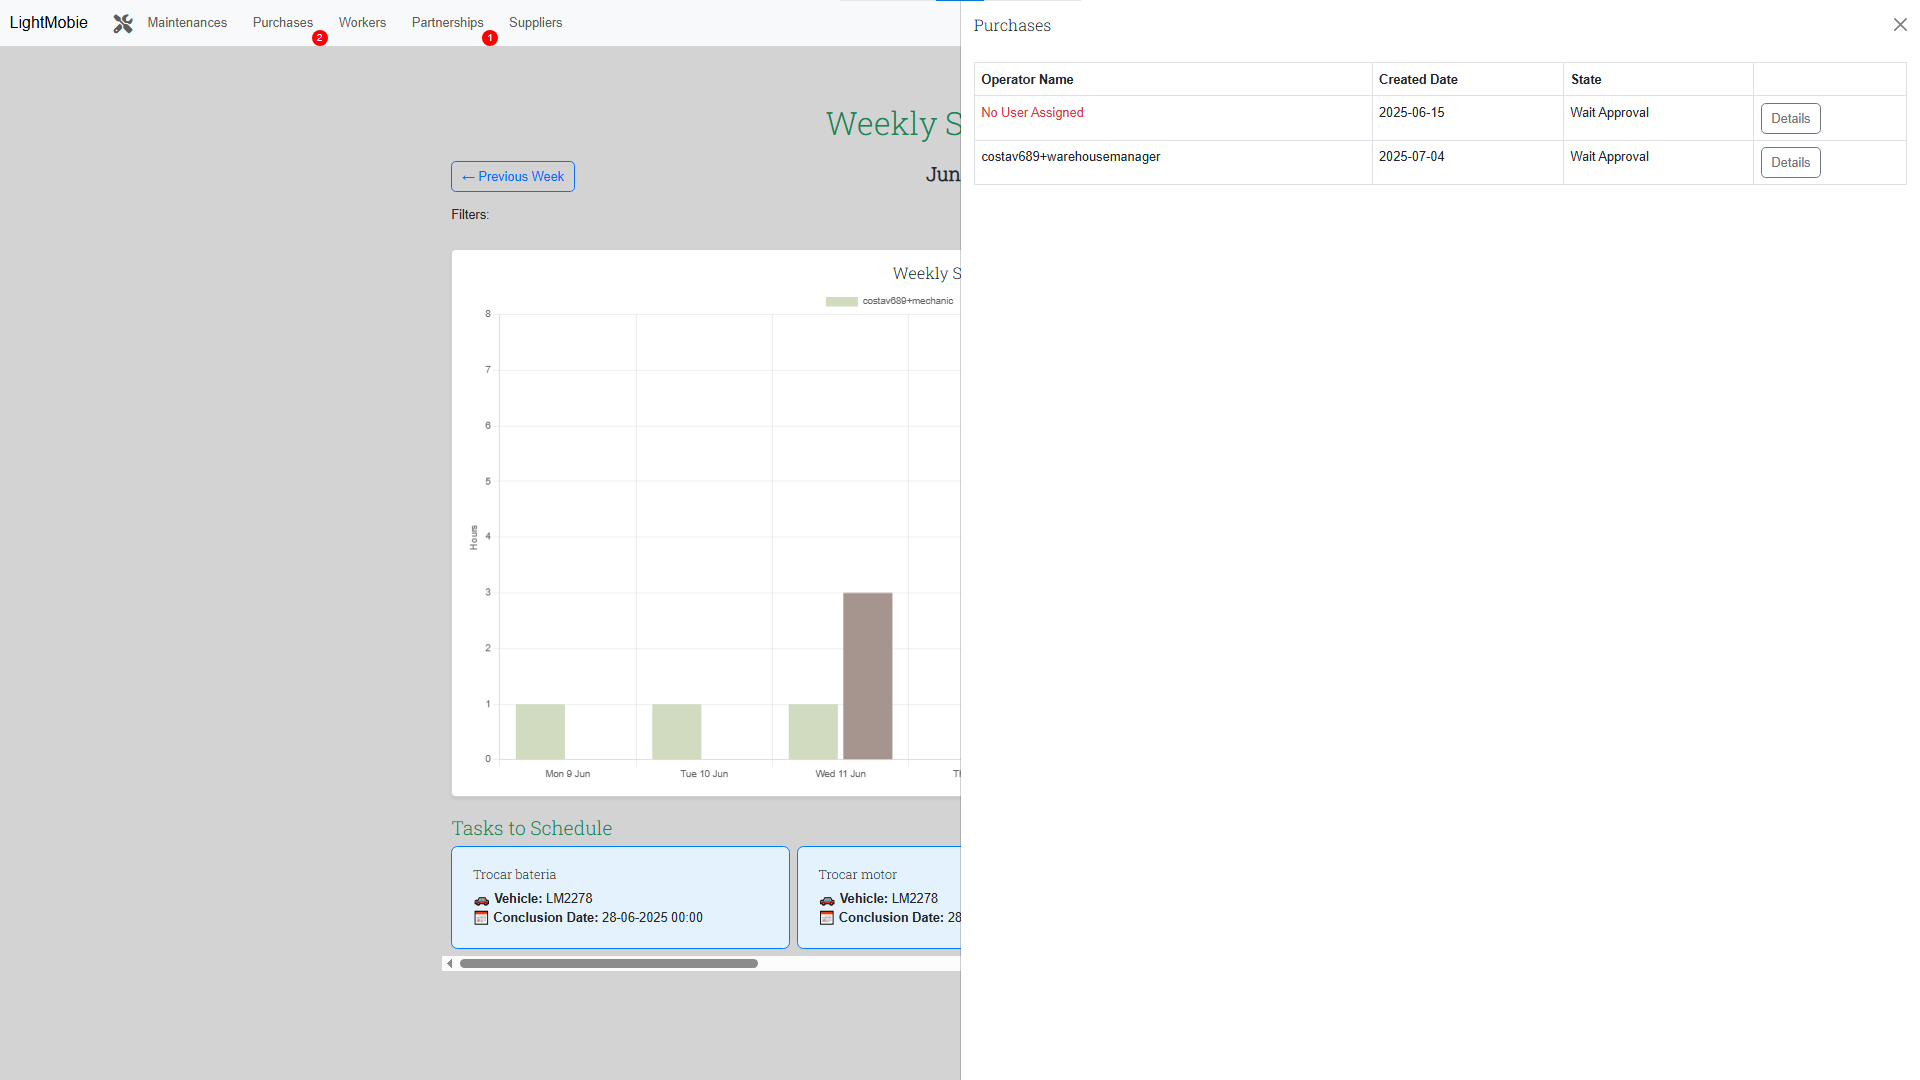
\includegraphics[width=\textwidth]{figs/Implementation/workshopmanager/purchaseList}
  \label{fig:figure2}
\end{figure}



\begin{figure}[h]
  \caption{Purchase request details.}
  \centering
  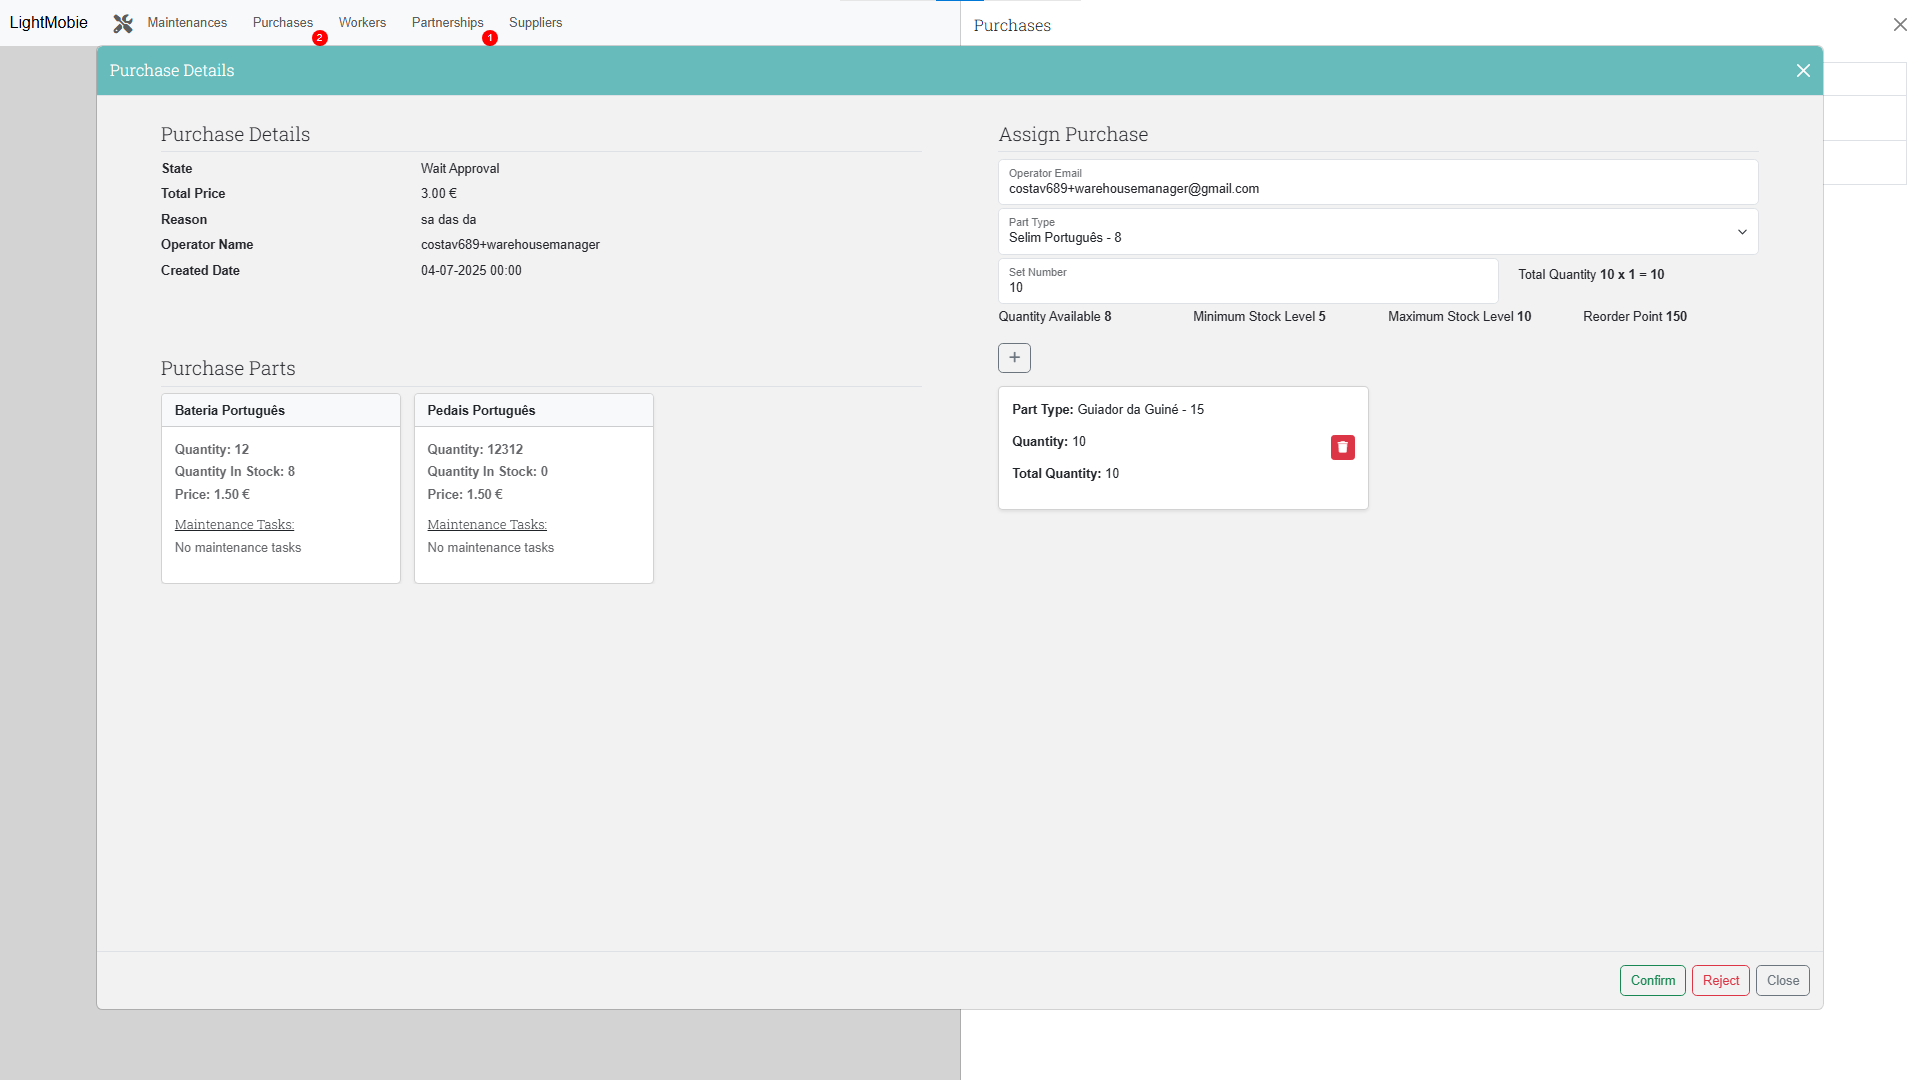
\includegraphics[width=\textwidth]{figs/Implementation/workshopmanager/purchaseDetails}
  \label{fig:figure2}
\end{figure}

Returning to the home page, the menu next option is the purchases.
By clicking in this button, it will open the list of purchases that need to be authorized by the manager.
When opening the details of a purchase will show a modal with the information of the purchase on the left side and a form on the right.
The form allows the workshop manager to add more parts to the purchase and assign the purchase to a operator if it isn't assigned to anyone.
To authorize or reject the purchase the workshop manager can do that by clicking on the button "Confirmar" or "Reject", respectively, to accomplish this (Use Case 4.2 – Authorize purchase)

% \begin{figure}[h]
%   \caption{Transaction list.}
%   \centering
%   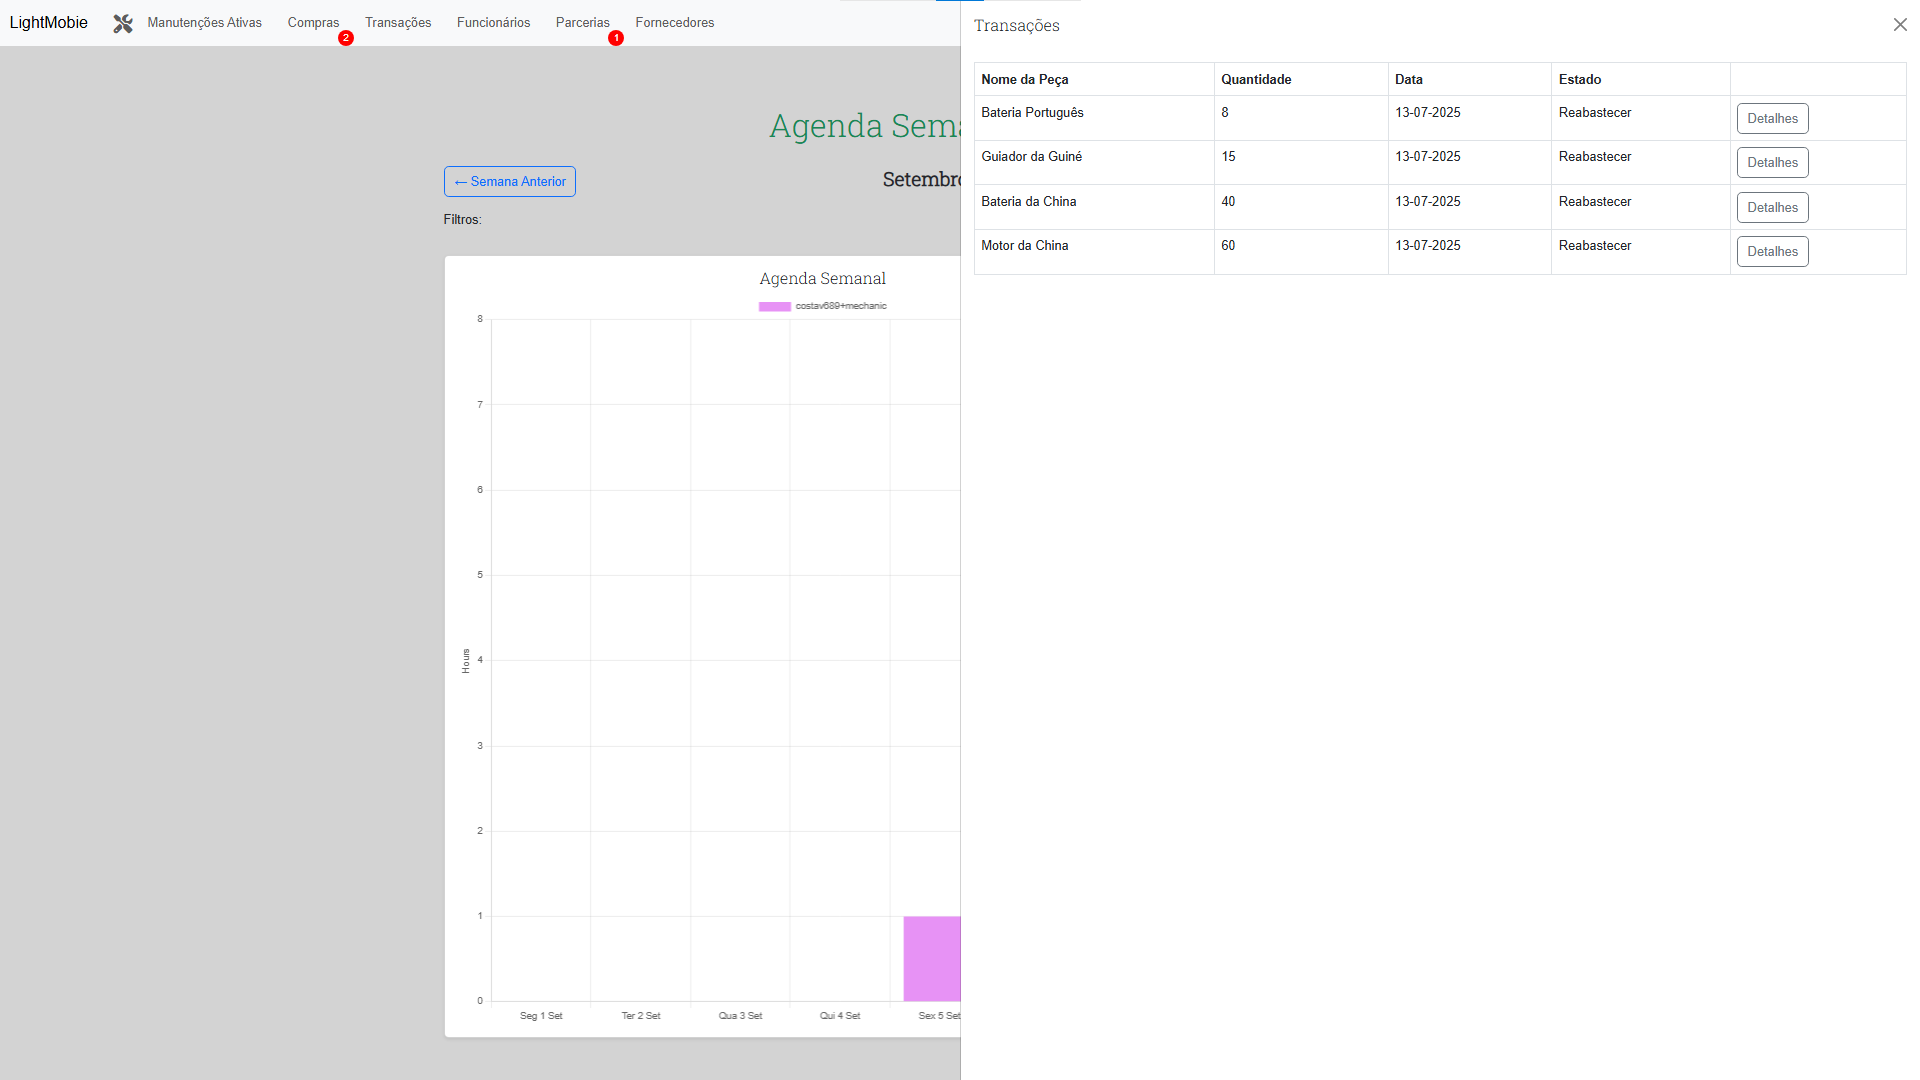
\includegraphics[width=\textwidth]{figs/Implementation/workshopmanager/transactionList}
%   \label{fig:figure2}
% \end{figure}

% Returning to the home page, the next offcanvas of the menu is the "Transações" which are the transaction of the parts in the inventory.
% By clicking on this button will show the \ref.


\begin{figure}[h]
  \caption{Worker list.}
  \centering
  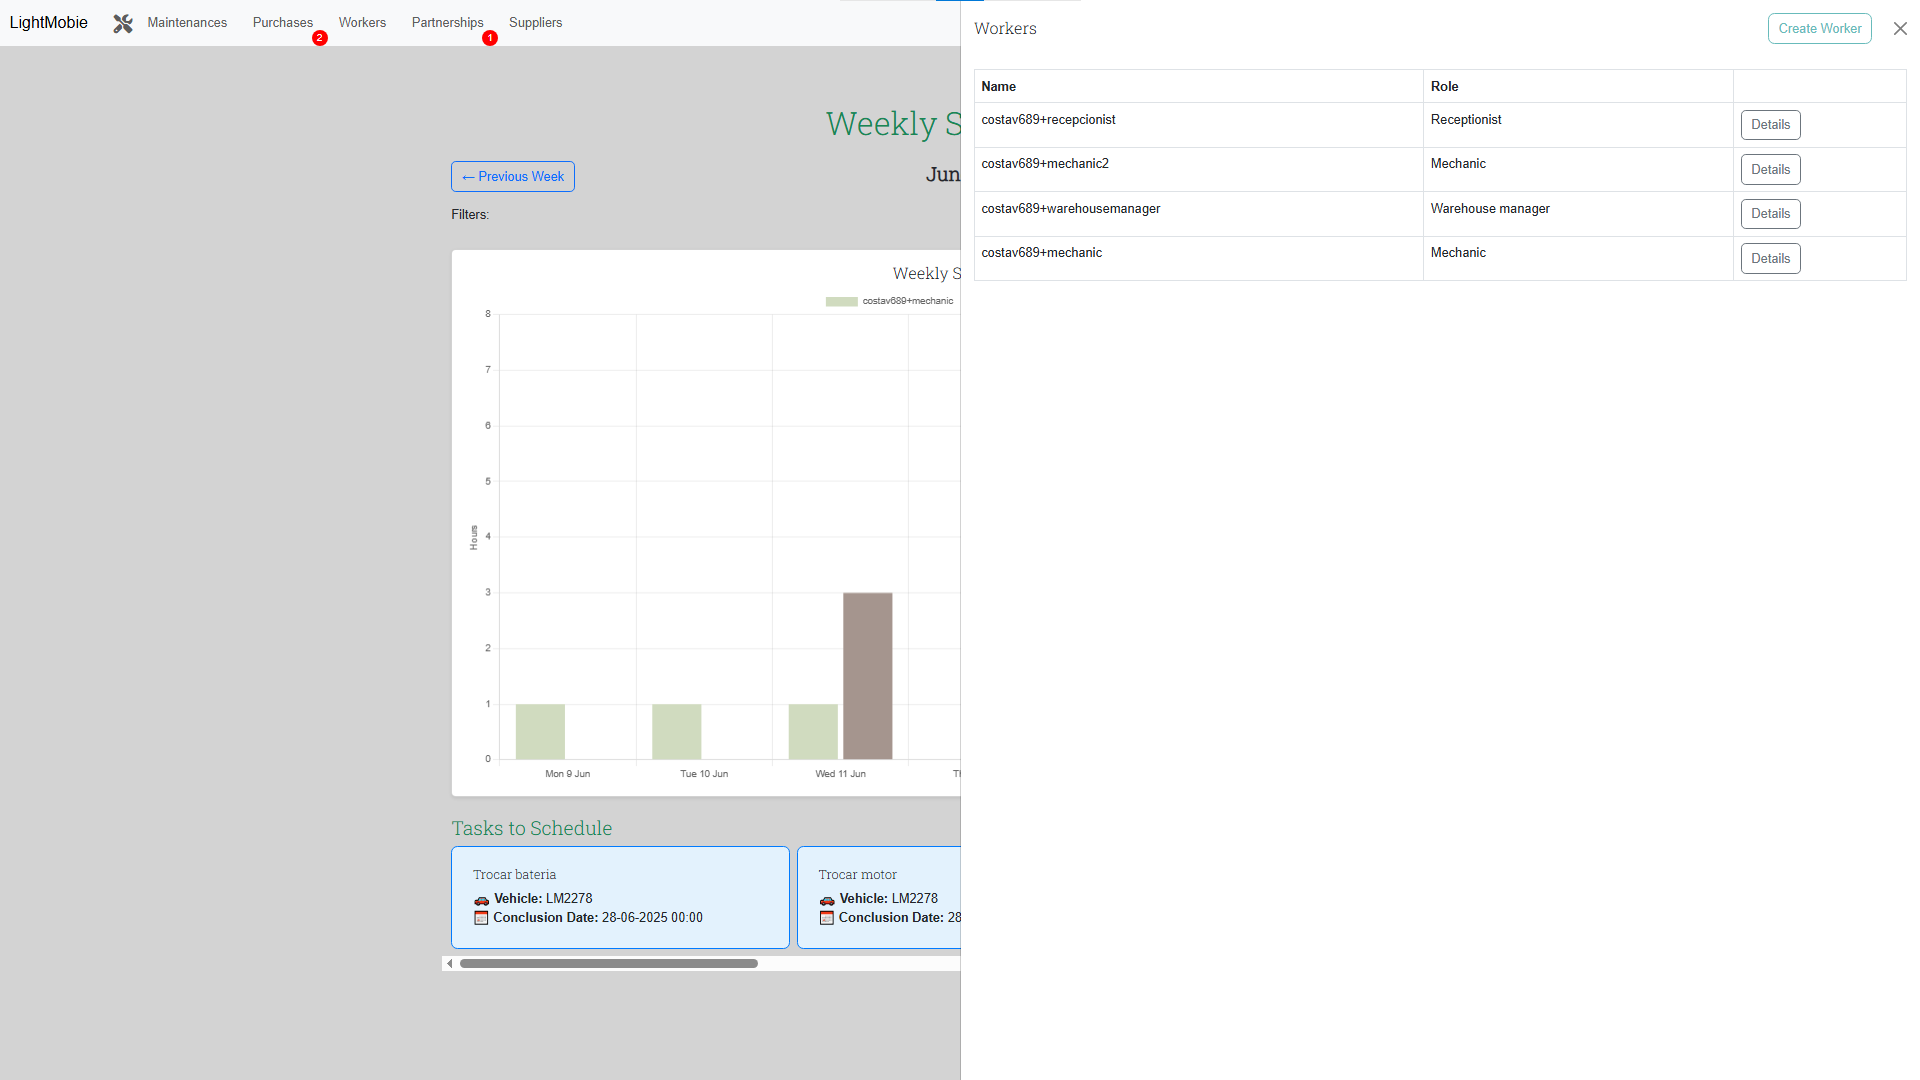
\includegraphics[width=\textwidth]{figs/Implementation/workshopmanager/workerList}
  \label{fig:figure2}
\end{figure}

Returning to the home page, the next offcanvas of the menu is the "Funcionários" which list the workers on the dealership.
By clicking on this button will show the \ref.

\begin{figure}[h]
  \caption{Worker details.}
  \centering
  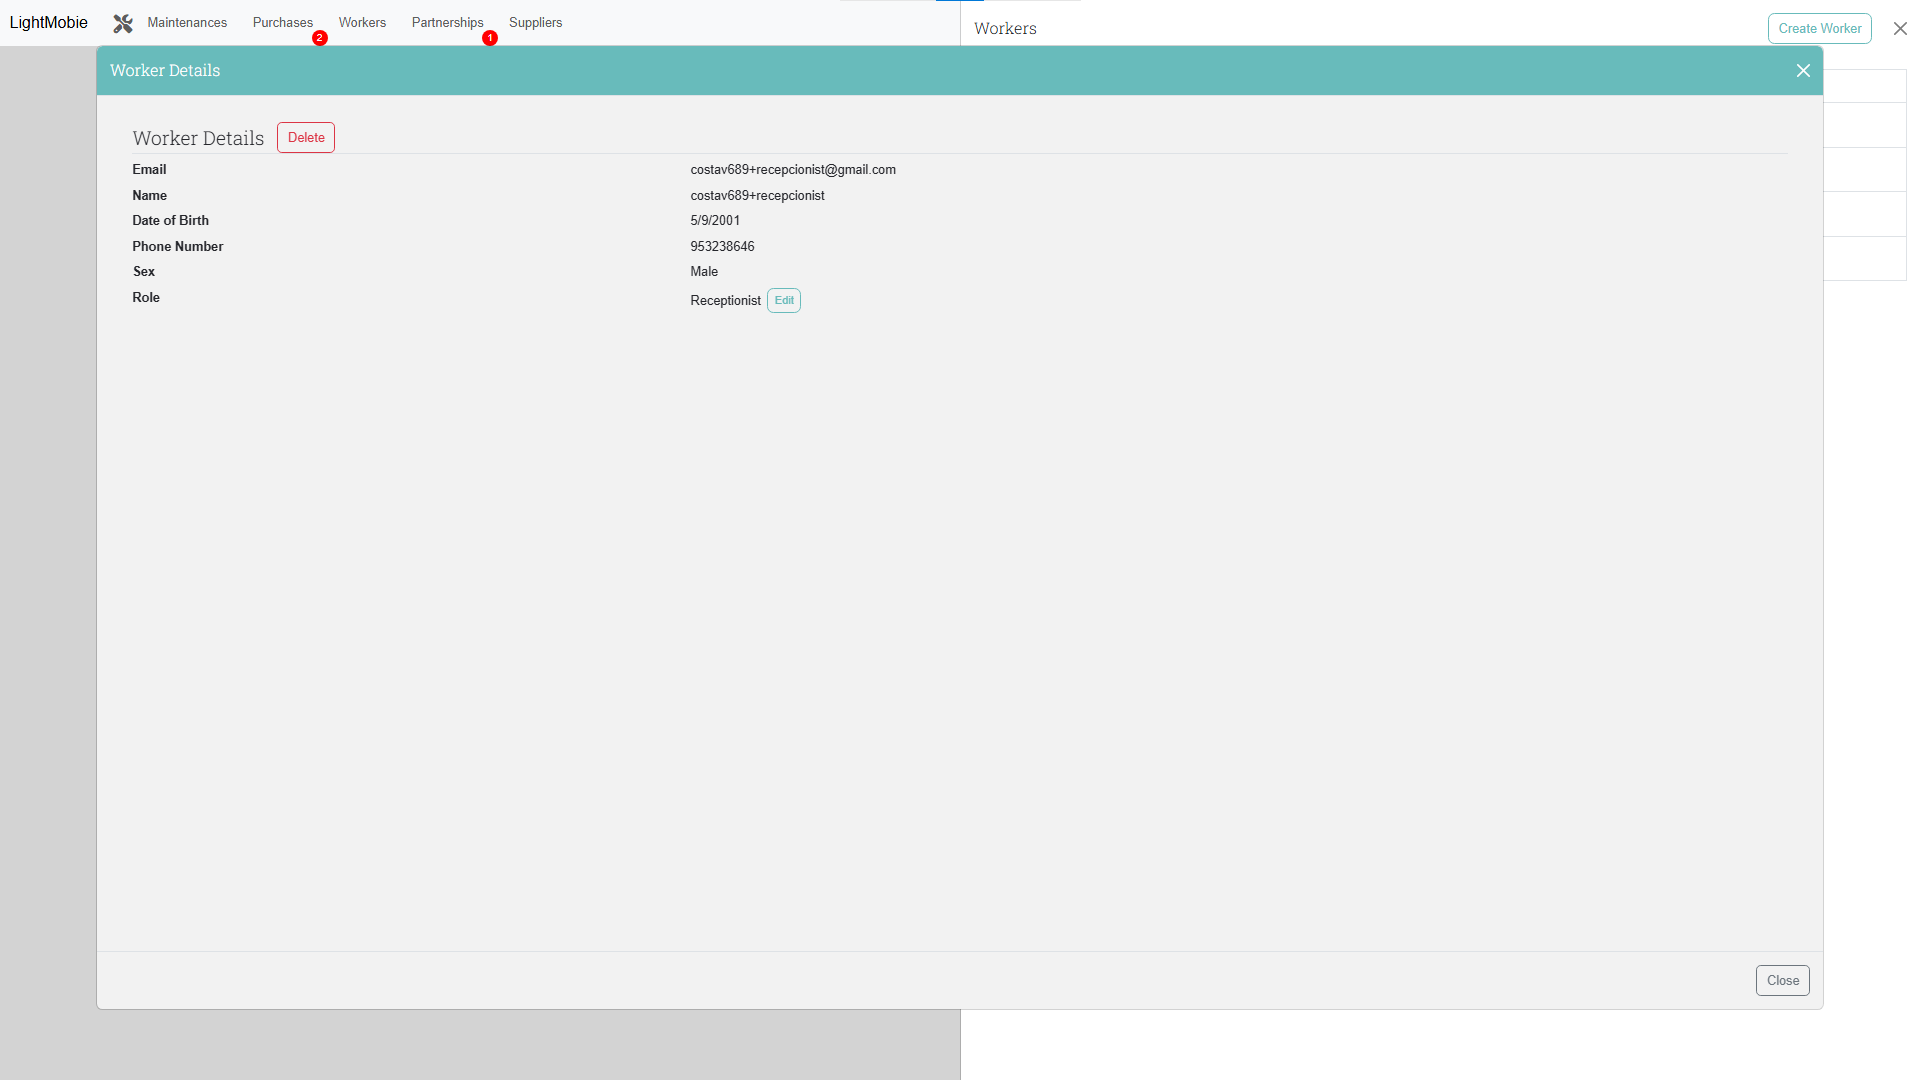
\includegraphics[width=\textwidth]{figs/Implementation/workshopmanager/workerDetails}
  \label{fig:figure2}
\end{figure}

This table shows the workers by email and there role. 
By cliking the details button, it will open a modal as seen in \ref.
In this modal, the manager can remove the worker, edit the role (Use Case 4.5 – Assign roles to employees) and also see the following information:
- the name of the worker
- the date of birth
- the phone number
- sex



\begin{figure}[h]
  \caption{Create worker.}
  \centering
  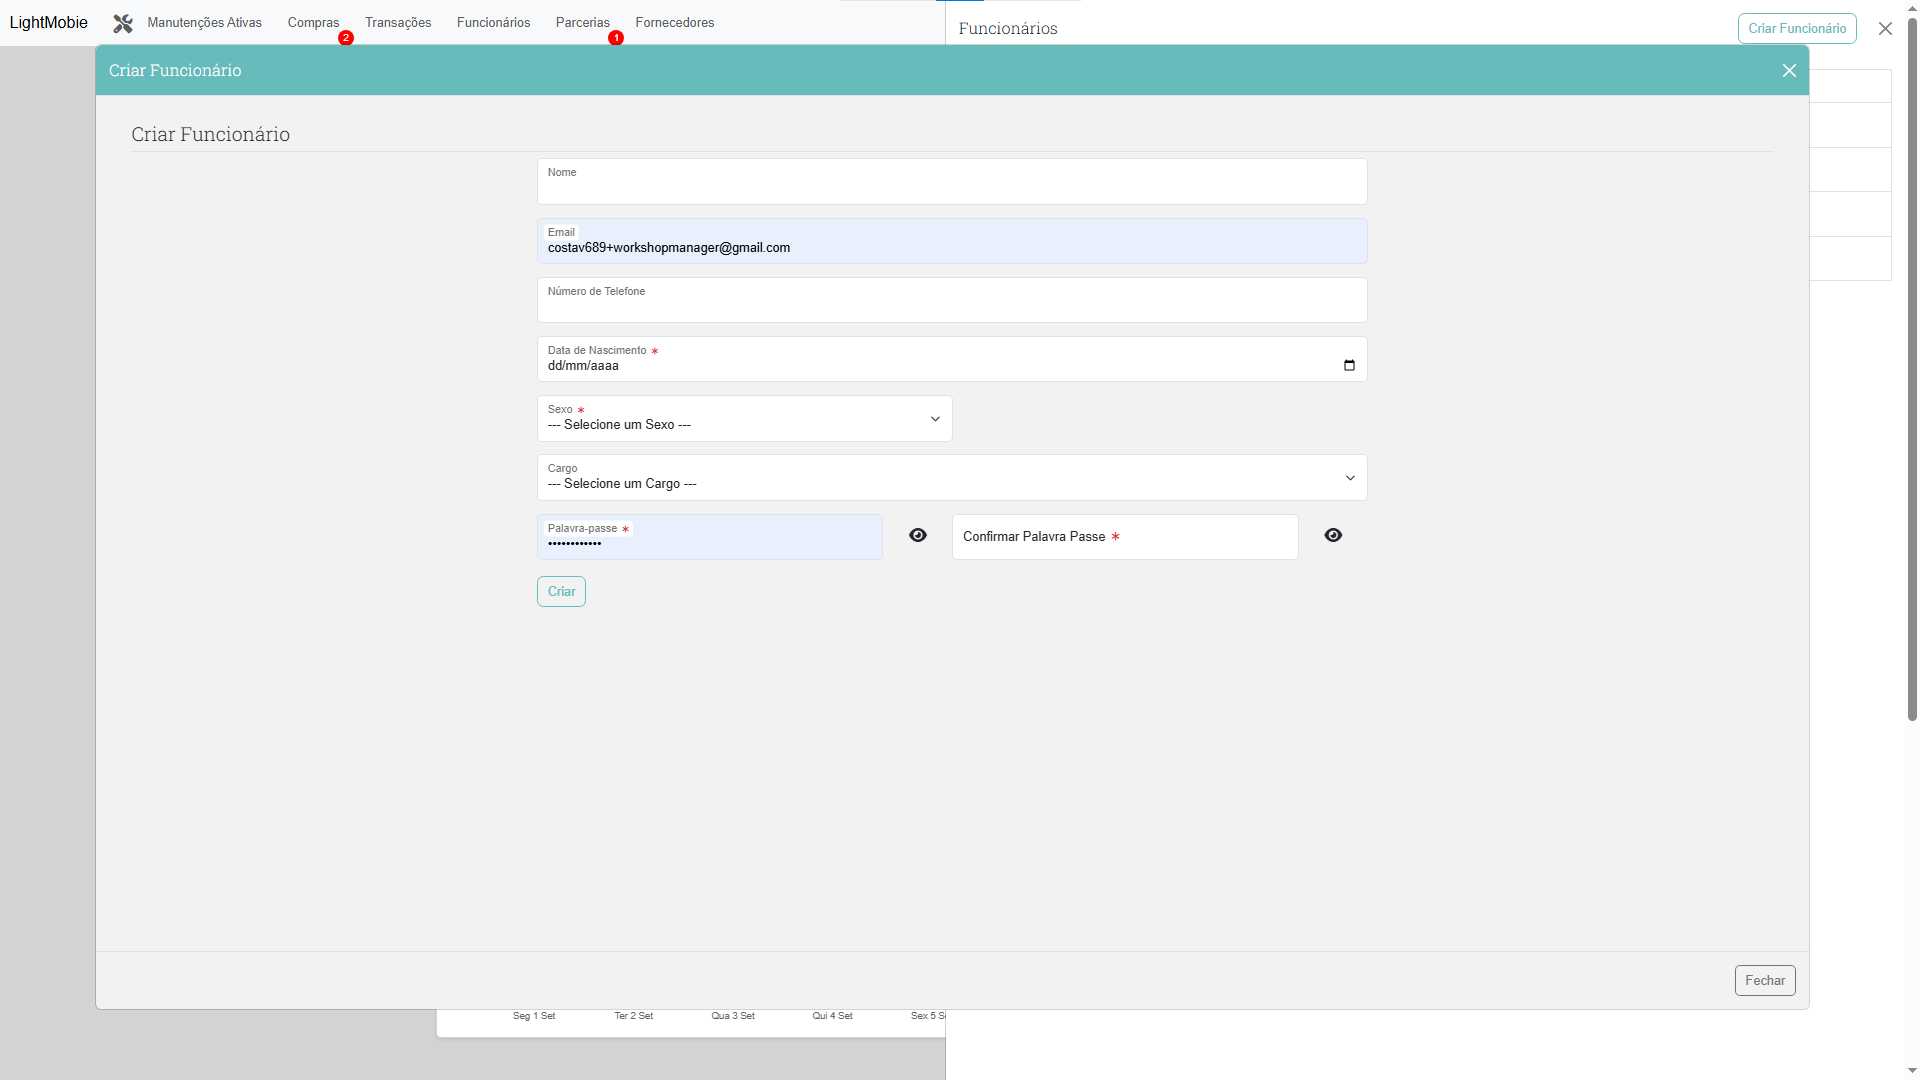
\includegraphics[width=\textwidth]{figs/Implementation/workshopmanager/workerCreate}
  \label{fig:figure2}
\end{figure}


In the list of the users there is also a button to create workers called "Criar Funcionário", that will open a modal as seen in \ref.
To create a worker must introduce:
- Name
- Email
- phone number
- Date of birth
- sex
- Role
- Password

After the user is created he must confirm his email in his email box.

\begin{figure}[h]
  \caption{Partnership list.}
  \centering
  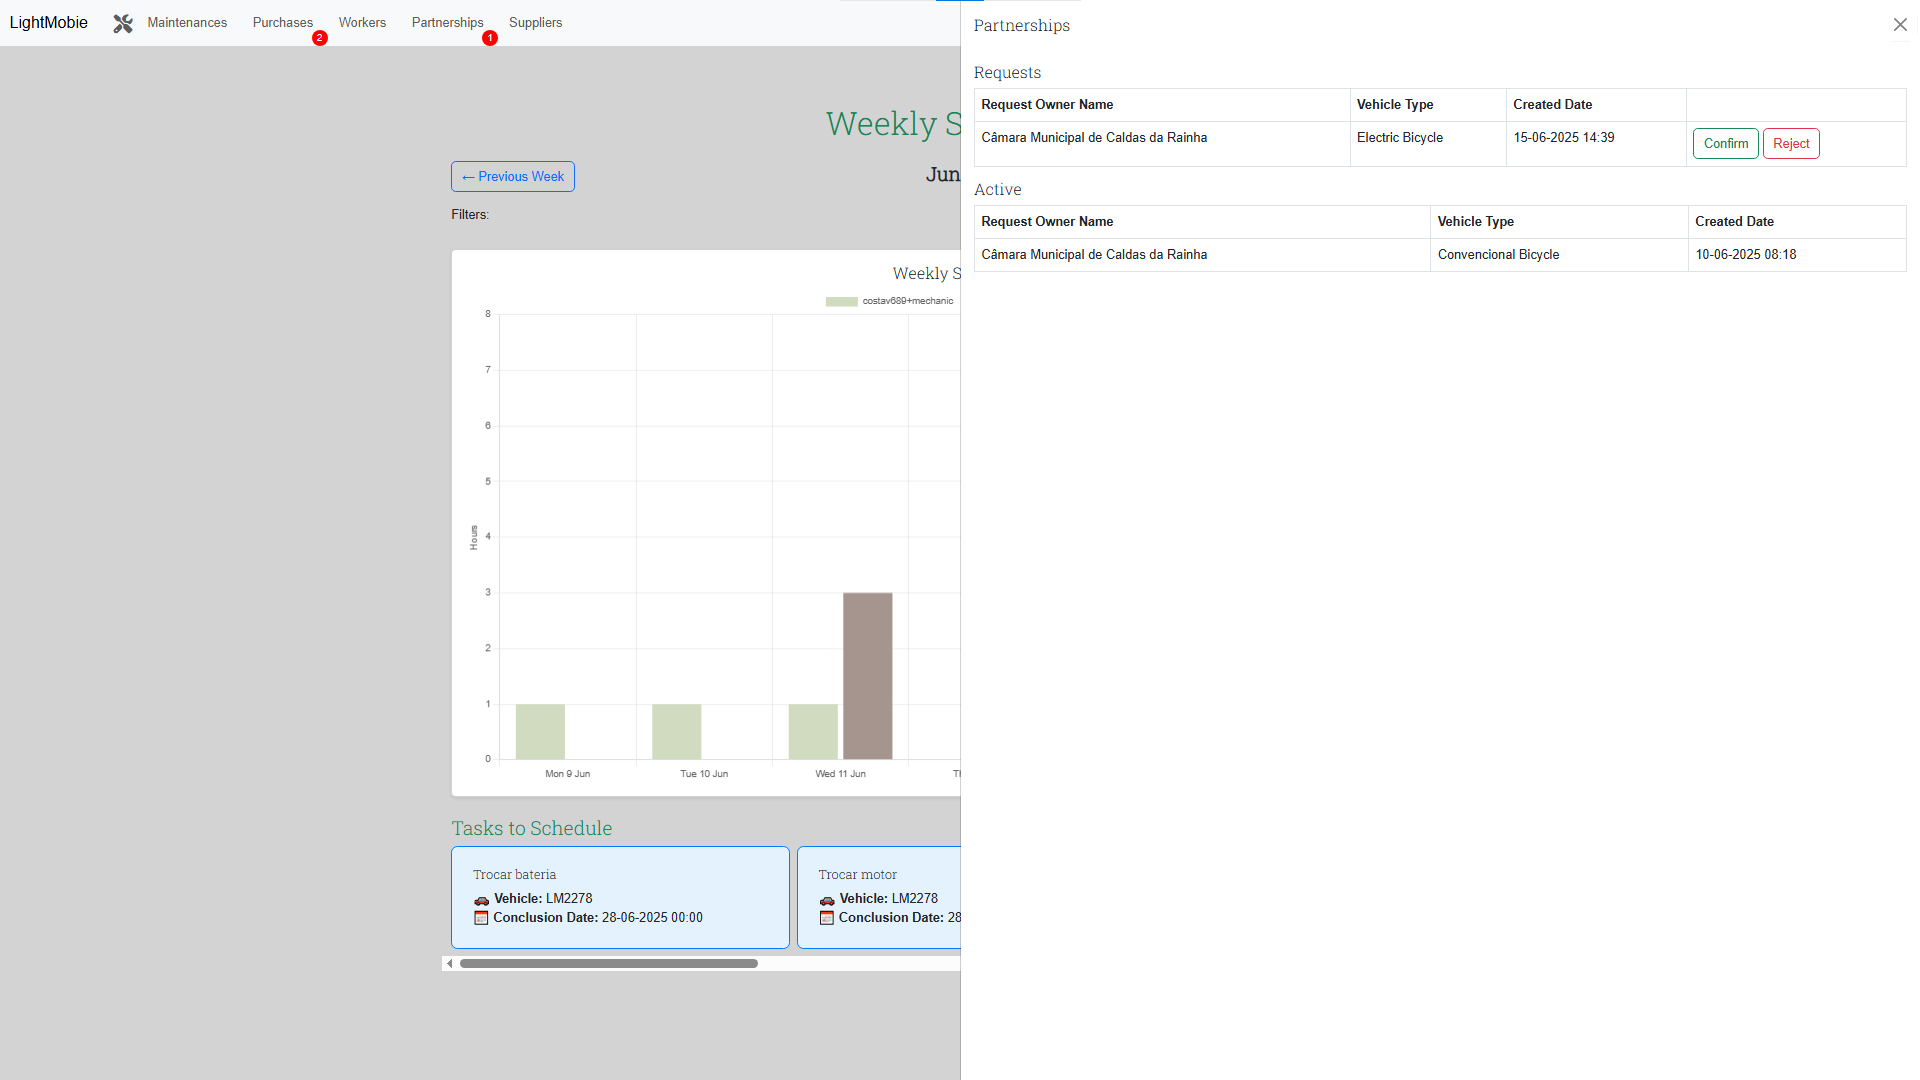
\includegraphics[width=\textwidth]{figs/Implementation/workshopmanager/partnershipList}
  \label{fig:figure2}
\end{figure}


Returning to the home page, the next menu option is the "Parceiros", that will open a modal like in \ref.
In this modal it shows two tables, the first one are the request from others bike sharing entities with:
- the name of the entity
- the type of vehicles the entity wants the dealership to maintain
- the date of creation of the request
- two buttons to confirm or reject the request (Use Case 4.8 – Accept/Reject partnership)

The next table shows all the partners of the dealership.

\begin{figure}[h]
  \caption{Supplier list.}
  \centering
  \includegraphics[width=\textwidth]{figs/Implementation/workshopmanager/supplierList}
  \label{fig:figure2}
\end{figure}

\begin{figure}[h]
  \caption{Supplier Details.}
  \centering
  \includegraphics[width=\textwidth]{figs/Implementation/workshopmanager/supplierDetails}
  \label{fig:figure2}
\end{figure}

The last menu option are the "Fornecedores", this offcanvas is the same as the warehouse operator.
It shows the suppliers and the information of the contracts of parts they supply, as seen in \ref and \ref.


\subsection{Client view}

\begin{figure}[h]
  \caption{Client home page with no active maintenance.}
  \centering
  \includegraphics[width=\textwidth]{figs/Implementation/client/MaintenanceNoState}
  \label{fig:figure2}
\end{figure}

\begin{figure}[h]
  \caption{Client Home page when he schedules a maintenance with the rececionist.}
  \centering
  \includegraphics[width=\textwidth]{figs/Implementation/client/MaintenanceState1}
  \label{fig:figure2}
\end{figure}

\begin{figure}[h]
  \caption{Client Home page when the vehicle evaluation is complete.}
  \centering
  \includegraphics[width=\textwidth]{figs/Implementation/client/MaintenanceState2}
  \label{fig:figure2}
\end{figure}


\begin{figure}[h]
  \caption{Client Home page when the maintenance is approved.}
  \centering
  \includegraphics[width=\textwidth]{figs/Implementation/client/MaintenanceState3}
  \label{fig:figure2}
\end{figure}

\begin{figure}[h]
  \caption{Client Home page when the maintenance tasks are completed and the client can go take the vehicle.}
  \centering
  \includegraphics[width=\textwidth]{figs/Implementation/client/MaintenanceState4}
  \label{fig:figure2}
\end{figure}

\begin{figure}[h]
  \caption{Client Home page when the vehicle after the vehicle is delivered to the client.}
  \centering
  \includegraphics[width=\textwidth]{figs/Implementation/client/MaintenanceState5}
  \label{fig:figure2}
\end{figure}


In this view the layout is used for a phone as seen in \ref.
After the user contacts a dealership to mark a maintenance to the vehicle, it will show the view in \ref, where the user can see the date for the vehicle evaluation.
After tge evaluation it will show the view in \ref, where the user can see the tasks shown by the user and, after the maintenance approval, it will show this view \ref, where the user can track which tasks are completed or not.
Finally after all the task are completed it will show this view \ref and after  the vehicle is delivered this view (\ref), where the user is able to rate the service provided by the dealership.

\begin{figure}[h]
  \caption{List of completed maintenances of the client.}
  \centering
  \includegraphics[width=\textwidth]{figs/Implementation/client/MaintenanceHistory}
  \label{fig:figure2}
\end{figure}
The client in this app can also see the history of maintenance done to his vehicles (Use Case 5.5 – View maintenance history), as in \ref.
In this page the client can filter the maintenances by vehicle, dealership and date, as seen in \ref.
Also the client can download the report of the maintenance that is the same that the workshop manager sees (\ref) and see more information on maintenance details, as seen in \ref and \ref.

\begin{figure}[h]
  \caption{Details of a maintenance example the tab of information.}
  \centering
  \includegraphics[width=\textwidth]{figs/Implementation/client/MaintenanceDetailsInfo}
  \label{fig:figure2}
\end{figure}


\begin{figure}[h]
  \caption{Details of a maintenance example the list of task.}
  \centering
  \includegraphics[width=\textwidth]{figs/Implementation/client/MaintenanceDetailsTasks}
  \label{fig:figure2}
\end{figure}


\subsection{Administrator view}


\begin{figure}[h]
  \caption{Parts type list.}
  \centering
  \includegraphics[width=\textwidth]{figs/Implementation/dealershipAdmin/partsIndex}
  \label{fig:figure2}
\end{figure}


\begin{figure}[h]
  \caption{Parts type details.}
  \centering
  \includegraphics[width=\textwidth]{figs/Implementation/dealershipAdmin/partsDetails}
  \label{fig:figure2}
\end{figure}
The administrator view is used to set the information of the system, namely the existing parts, the tasks and eval task.
When the administrator logs in his account he gets a list of the diferentes types of parts that exist as seen in figure \ref.
In this page the administrator can create, delete, edit or view the existing parts.
By clicking in the button "Detalhes" of a row show the information about a part, as in \ref.

\begin{figure}[h]
  \caption{Parts type edit.}
  \centering
  \includegraphics[width=\textwidth]{figs/Implementation/dealershipAdmin/partsEdit}
  \label{fig:figure2}
\end{figure}

By clicking in the button "edit" of a row show a form with the information about the part, as in \ref.

\begin{figure}[h]
  \caption{Parts type delete.}
  \centering
  \includegraphics[width=\textwidth]{figs/Implementation/dealershipAdmin/partsDelete}
  \label{fig:figure2}
\end{figure}


By clicking in the button "delete" of a row show a form with the information about the part and a button to delete it, as in \ref.



\begin{figure}[h]
  \caption{Parts type create.}
  \centering
  \includegraphics[width=\textwidth]{figs/Implementation/dealershipAdmin/partsCreate}
  \label{fig:figure2}
\end{figure}

By clicking in the button "create" in the top of the table it shows the form of the edit empty, as in \ref.


\begin{figure}[h]
  \caption{Task type list index.}
  \centering
  \includegraphics[width=\textwidth]{figs/Implementation/dealershipAdmin/taskIndex}
  \label{fig:figure2}
\end{figure}

\begin{figure}[h]
  \caption{Task type edit.}
  \centering
  \includegraphics[width=\textwidth]{figs/Implementation/dealershipAdmin/taskEdit}
  \label{fig:figure2}
\end{figure}


\begin{figure}[h]
  \caption{Task type details.}
  \centering
  \includegraphics[width=\textwidth]{figs/Implementation/dealershipAdmin/taskDetails}
  \label{fig:figure2}
\end{figure}

 
\begin{figure}[h]
  \caption{Task type delete.}
  \centering
  \includegraphics[width=\textwidth]{figs/Implementation/dealershipAdmin/taskDelete}
  \label{fig:figure2}
\end{figure}

\begin{figure}[h]
  \caption{Task type create.}
  \centering
  \includegraphics[width=\textwidth]{figs/Implementation/dealershipAdmin/taskCreate}
  \label{fig:figure2}
\end{figure}


\begin{figure}[h]
  \caption{Eval task list index.}
  \centering
  \includegraphics[width=\textwidth]{figs/Implementation/dealershipAdmin/evalIndex}
  \label{fig:figure2}

\end{figure}
\begin{figure}[h]
  \caption{Eval task create.}
  \centering
  \includegraphics[width=\textwidth]{figs/Implementation/dealershipAdmin/evalCreate}
  \label{fig:figure2}
\end{figure}

\begin{figure}[h]
  \caption{Eval task delete.}
  \centering
  \includegraphics[width=\textwidth]{figs/Implementation/dealershipAdmin/evalDelete}
  \label{fig:figure2}
\end{figure}

\begin{figure}[h]
  \caption{Eval task details.}
  \centering
  \includegraphics[width=\textwidth]{figs/Implementation/dealershipAdmin/evalDetails}
  \label{fig:figure2}
\end{figure}

\begin{figure}[h]
  \caption{Eval task edit.}
  \centering
  \includegraphics[width=\textwidth]{figs/Implementation/dealershipAdmin/evalEdit}
  \label{fig:figure2}
\end{figure}


This layout is the same used for the tasks, as seen in \ref, \ref, \ref e \ref, and for eval tasks, as seen in \ref, \ref, \ref e \ref.
The design of this view is to see the information the more pratical and efficient possible.






